\documentclass[10pt,twocolumn,letterpaper]{article}

\usepackage{cvpr}
\usepackage{times}
\usepackage{epsfig}
\usepackage{graphicx}
\usepackage{amsmath}
\usepackage{amssymb}
\usepackage{subfigure}
\usepackage{epstopdf}
\usepackage{multirow}
\usepackage{graphicx}  %ziqiang
\usepackage{pythonhighlight}   %ziqiang
\usepackage{mathtools} %ziqiang

% Include other packages here, before hyperref.

% If you comment hyperref and then uncomment it, you should delete
% egpaper.aux before re-running latex.  (Or just hit 'q' on the first latex
% run, let it finish, and you should be clear).
\usepackage[breaklinks=true,bookmarks=false]{hyperref}

\cvprfinalcopy % *** Uncomment this line for the final submission

\def\cvprPaperID{****} % *** Enter the CVPR Paper ID here
\def\httilde{\mbox{\tt\raisebox{-.5ex}{\symbol{126}}}}

% Pages are numbered in submission mode, and unnumbered in camera-ready
%\ifcvprfinal\pagestyle{empty}\fi
\setcounter{page}{1}
\begin{document}

%%%%%%%%% TITLE
\title{CMPE 264 - Project Assignment 2}

\author{Yanan Xie\\
{\tt\small yaxie@ucsc.edu}
% For a paper whose authors are all at the same institution,
% omit the following lines up until the closing ``}''.
% Additional authors and addresses can be added with ``\and'',
% just like the second author.
% To save space, use either the email address or home page, not both
\and
Ziqiang Wang\\
{\tt\small zwang232@ucsc.edu}
}

\maketitle
%\thispagestyle{empty}

%%%%%%%%% ABSTRACT

%%%%%%%%% BODY TEXT
\section{Camera radiometric calibration}
The first step of this project is to calibrate the camera. Since we are going to implement the plane-sweeping multiview stero, we have to know the intrinsic parameters and the distortion coefficients of the camera we use. The camera we used in the project is the Cannon 5D, after the calibration we use the same camera to take multiple views and implemented the plane-sweeping muliview stero. 


We learned from the tutorial that the distortion is composed of two differernt parts, radial distortion and tangential distortion. As for the radial distortion, we have 

$x_{distorted} = x(1+k_{1}r^{2}+k_{2}r^{4}+k_{3}r^{6})$\\
$y_{distorted} = y(1+k_{1}r^{2}+k_{2}r^{4}+k_{3}r^{6})$

As for the tangental distortion, we have 

$x_{distorted} = x+[2p_{1}xy+p_{2}(r^{2}+2x^{2})]$\\
$y_{distorted} = y+[p_{1}(r^{2}+2y^{2})+2p_{2}xy]$

So the distortion coefficients we need to find are $k_{1}$, $k_{2}$, $p_{1}$, $p_{2}$, $p_{3}$.

We also learned from the tutorial that the camera intrinsic matrix consist four degrees of freedoomthis instead of three. These are more than what we have learned about the distortion and the camera matrix, but we learned it and take it for the following project parts. 


We need a perfect flat surface of the chessboard to be as the standard world coordinate reference system. However, we tried to printed the chessboard picture and glue it onto the flat desk surface, then we take pictures and compute, but the outcome of the calibration is not idea to do undistortion since the printed piece of paper is not perfect flat. So finally we show the chessboard on the full-screen of our Macbook and take pictures and then compute, the intrinsic parameters we got this time is better, this is understandable since the screen is much more perfect flat than the printed paper, and we got much better result in the following undistortion step. There are two key points of taking the chessboard pictures we concluded as we try this process, first is we should full fill each picture we take with the whole chessboard, the second is the surface of the chessboard has to be prefect flat so that all the $Z$ coordinate of the chessboard point respect to the world reference system could be the same. All of these pictures we took for the chessboard is as shown in Figure \ref{fig:chessboard}.

As for the implementation of how to get the intrinsic paremeters, we adapted the $findChessboardCorners( )$ fucntion to find the chessboard corners in each picture we took, if the returned boolean value show that the corners was found in the picture then we add the corners into the $imgpoints[ ]$ list and accordingly make a pair of the world reference system coordinate in the $objpoints[ ]$ list. Then we pass the $imgpoints[ ]$ list and the $objpoints[ ]$ list to the $calibrateCamera( )$ function and we got the camera matrix and the distortion coefficients. 

The camera matrix K is 

$$\textbf{K} =
\begin{bmatrix}
2.83973773{\text e+}03&0.00000000{\text e+}00&1.38947081{\text e+}03\\
0.00000000{\text e+}00&2.83695500{\text e+}03&9.36984169{\text e+}02\\
0.00000000{\text e+}00&0.00000000{\text e+}00&1.00000000{\text e+}00 
\end{bmatrix}
$$

We also have the distortion coefficients after the computation, shown as below

$k_{1} = -0.12244297$, $k_{2} = 0.20499093$, $p_{1} = 0.00035033$, $p_{2} = -0.00058871$, $p_{3} = -0.13275741$

\begin{figure}[t]
\centering
\subfigure[Image 1]{
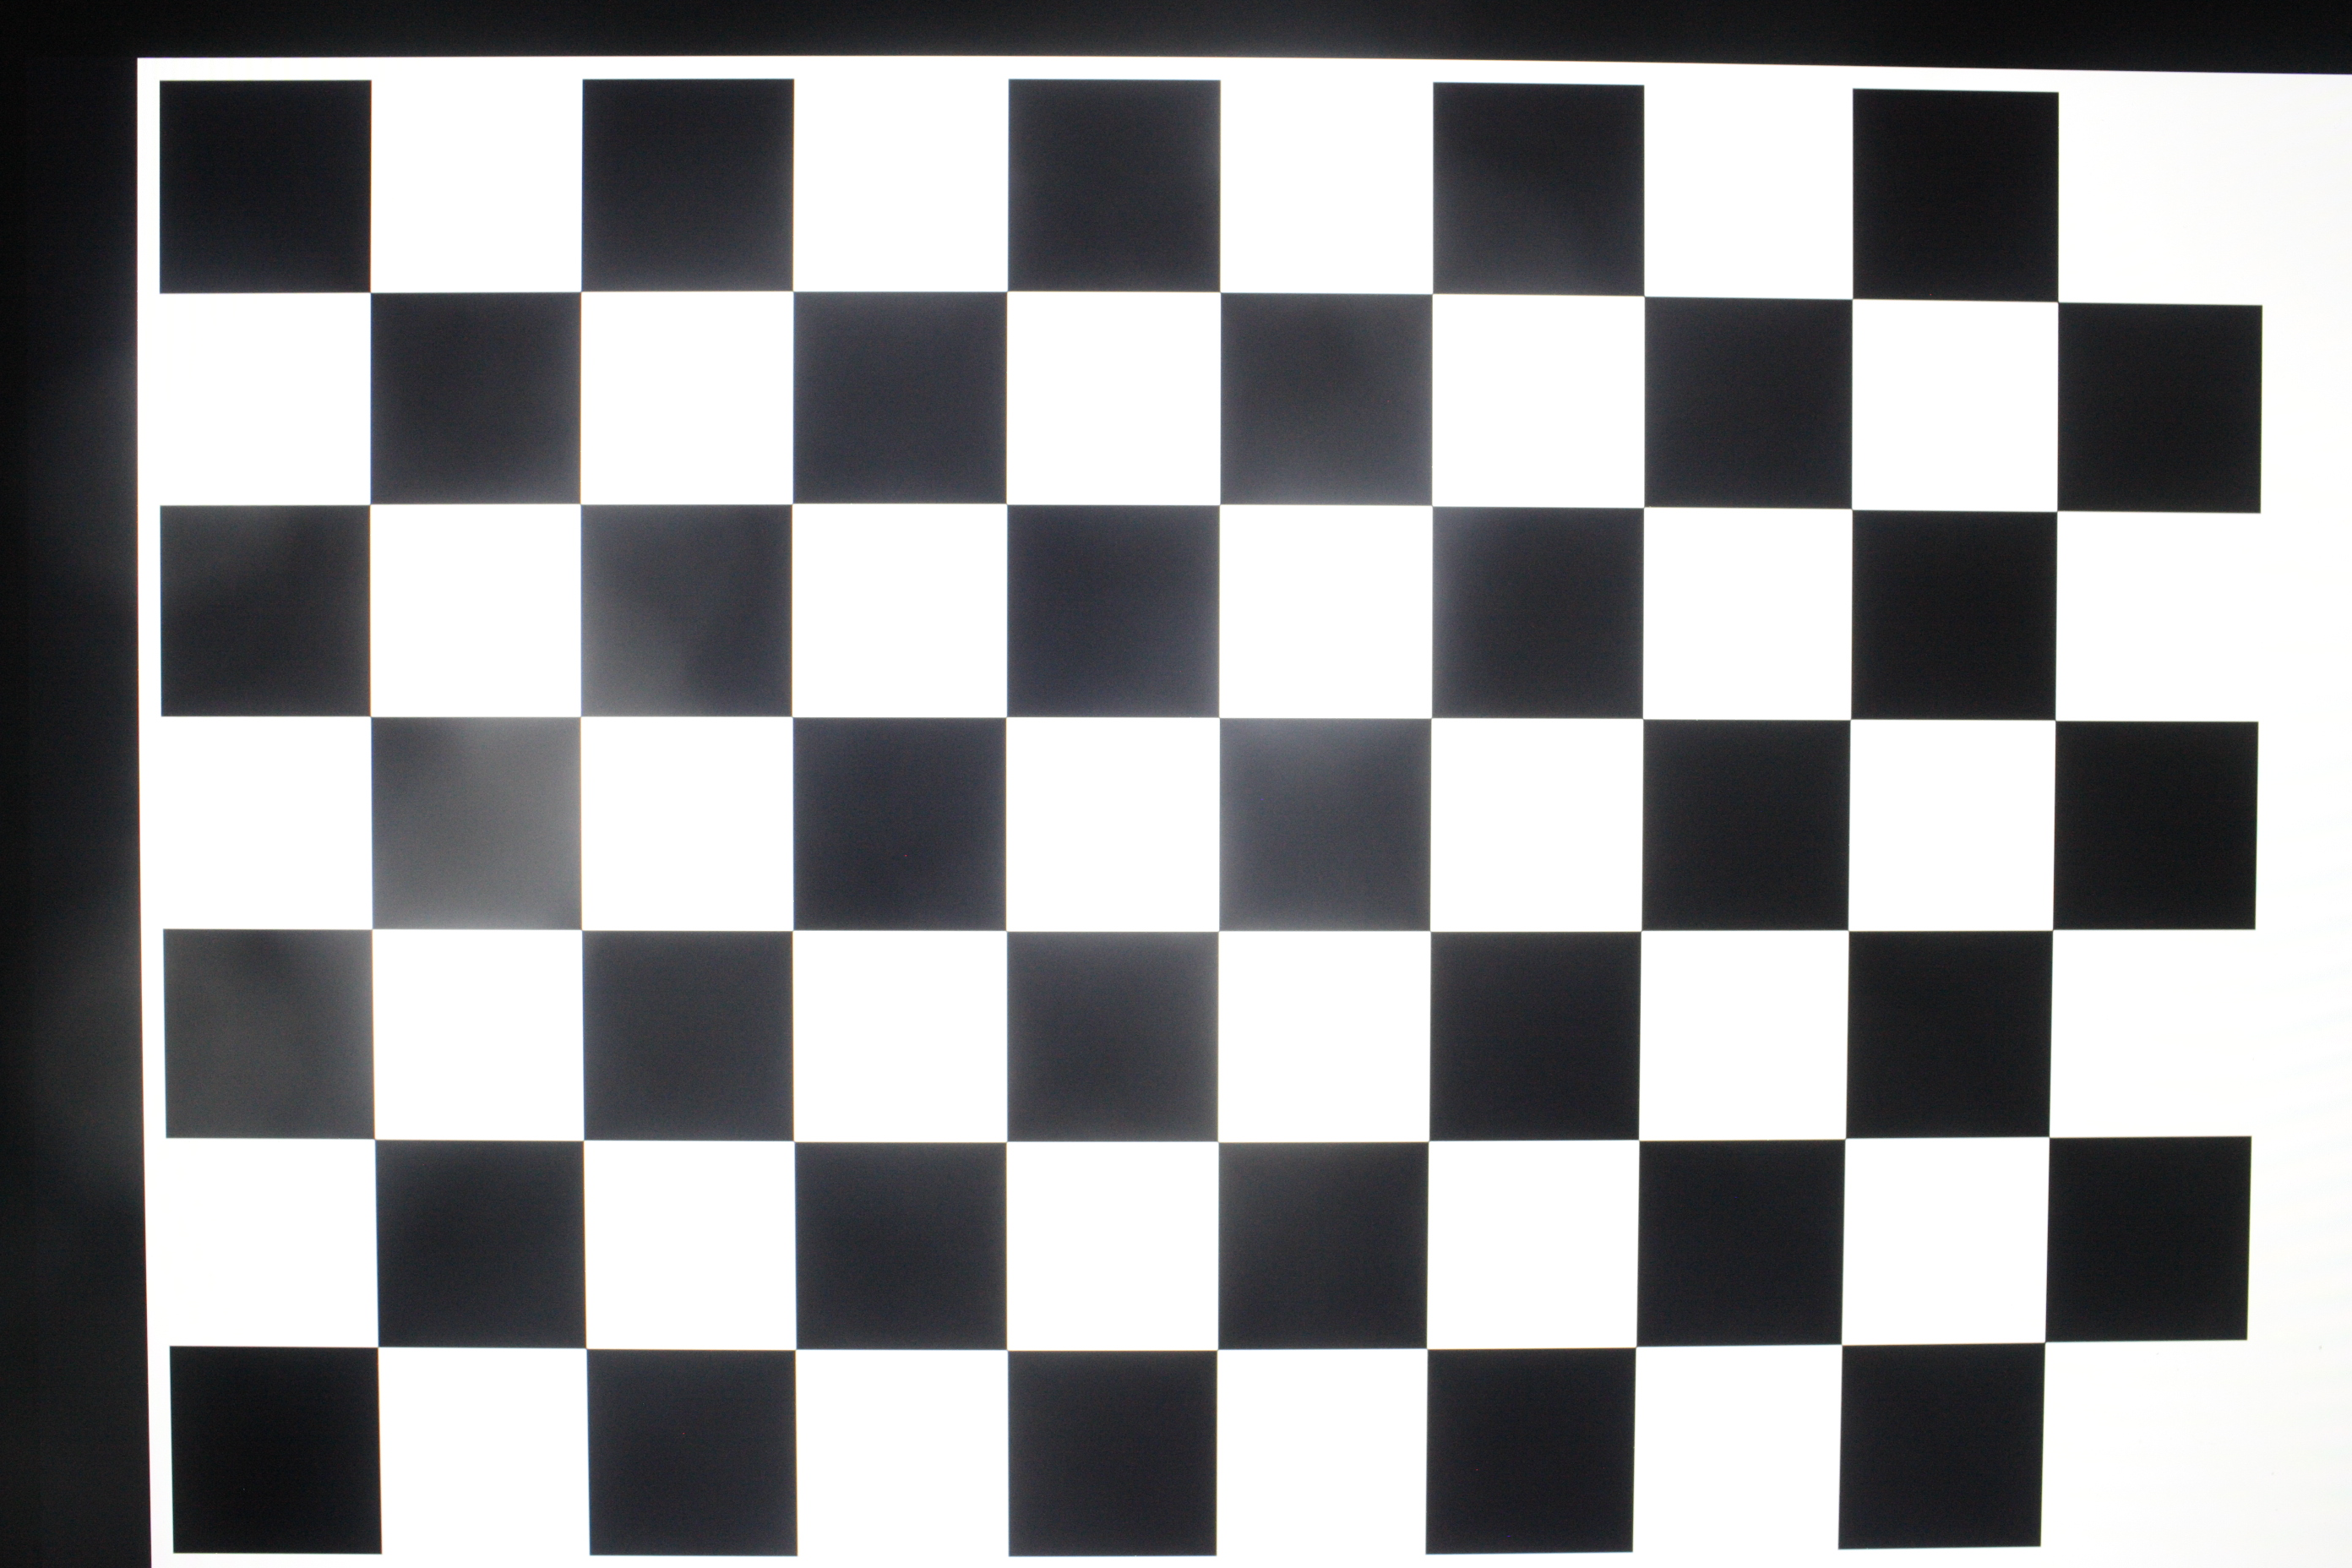
\includegraphics[width=.3\columnwidth]{images/chessboard/p1}
}
\subfigure[Image 2]{
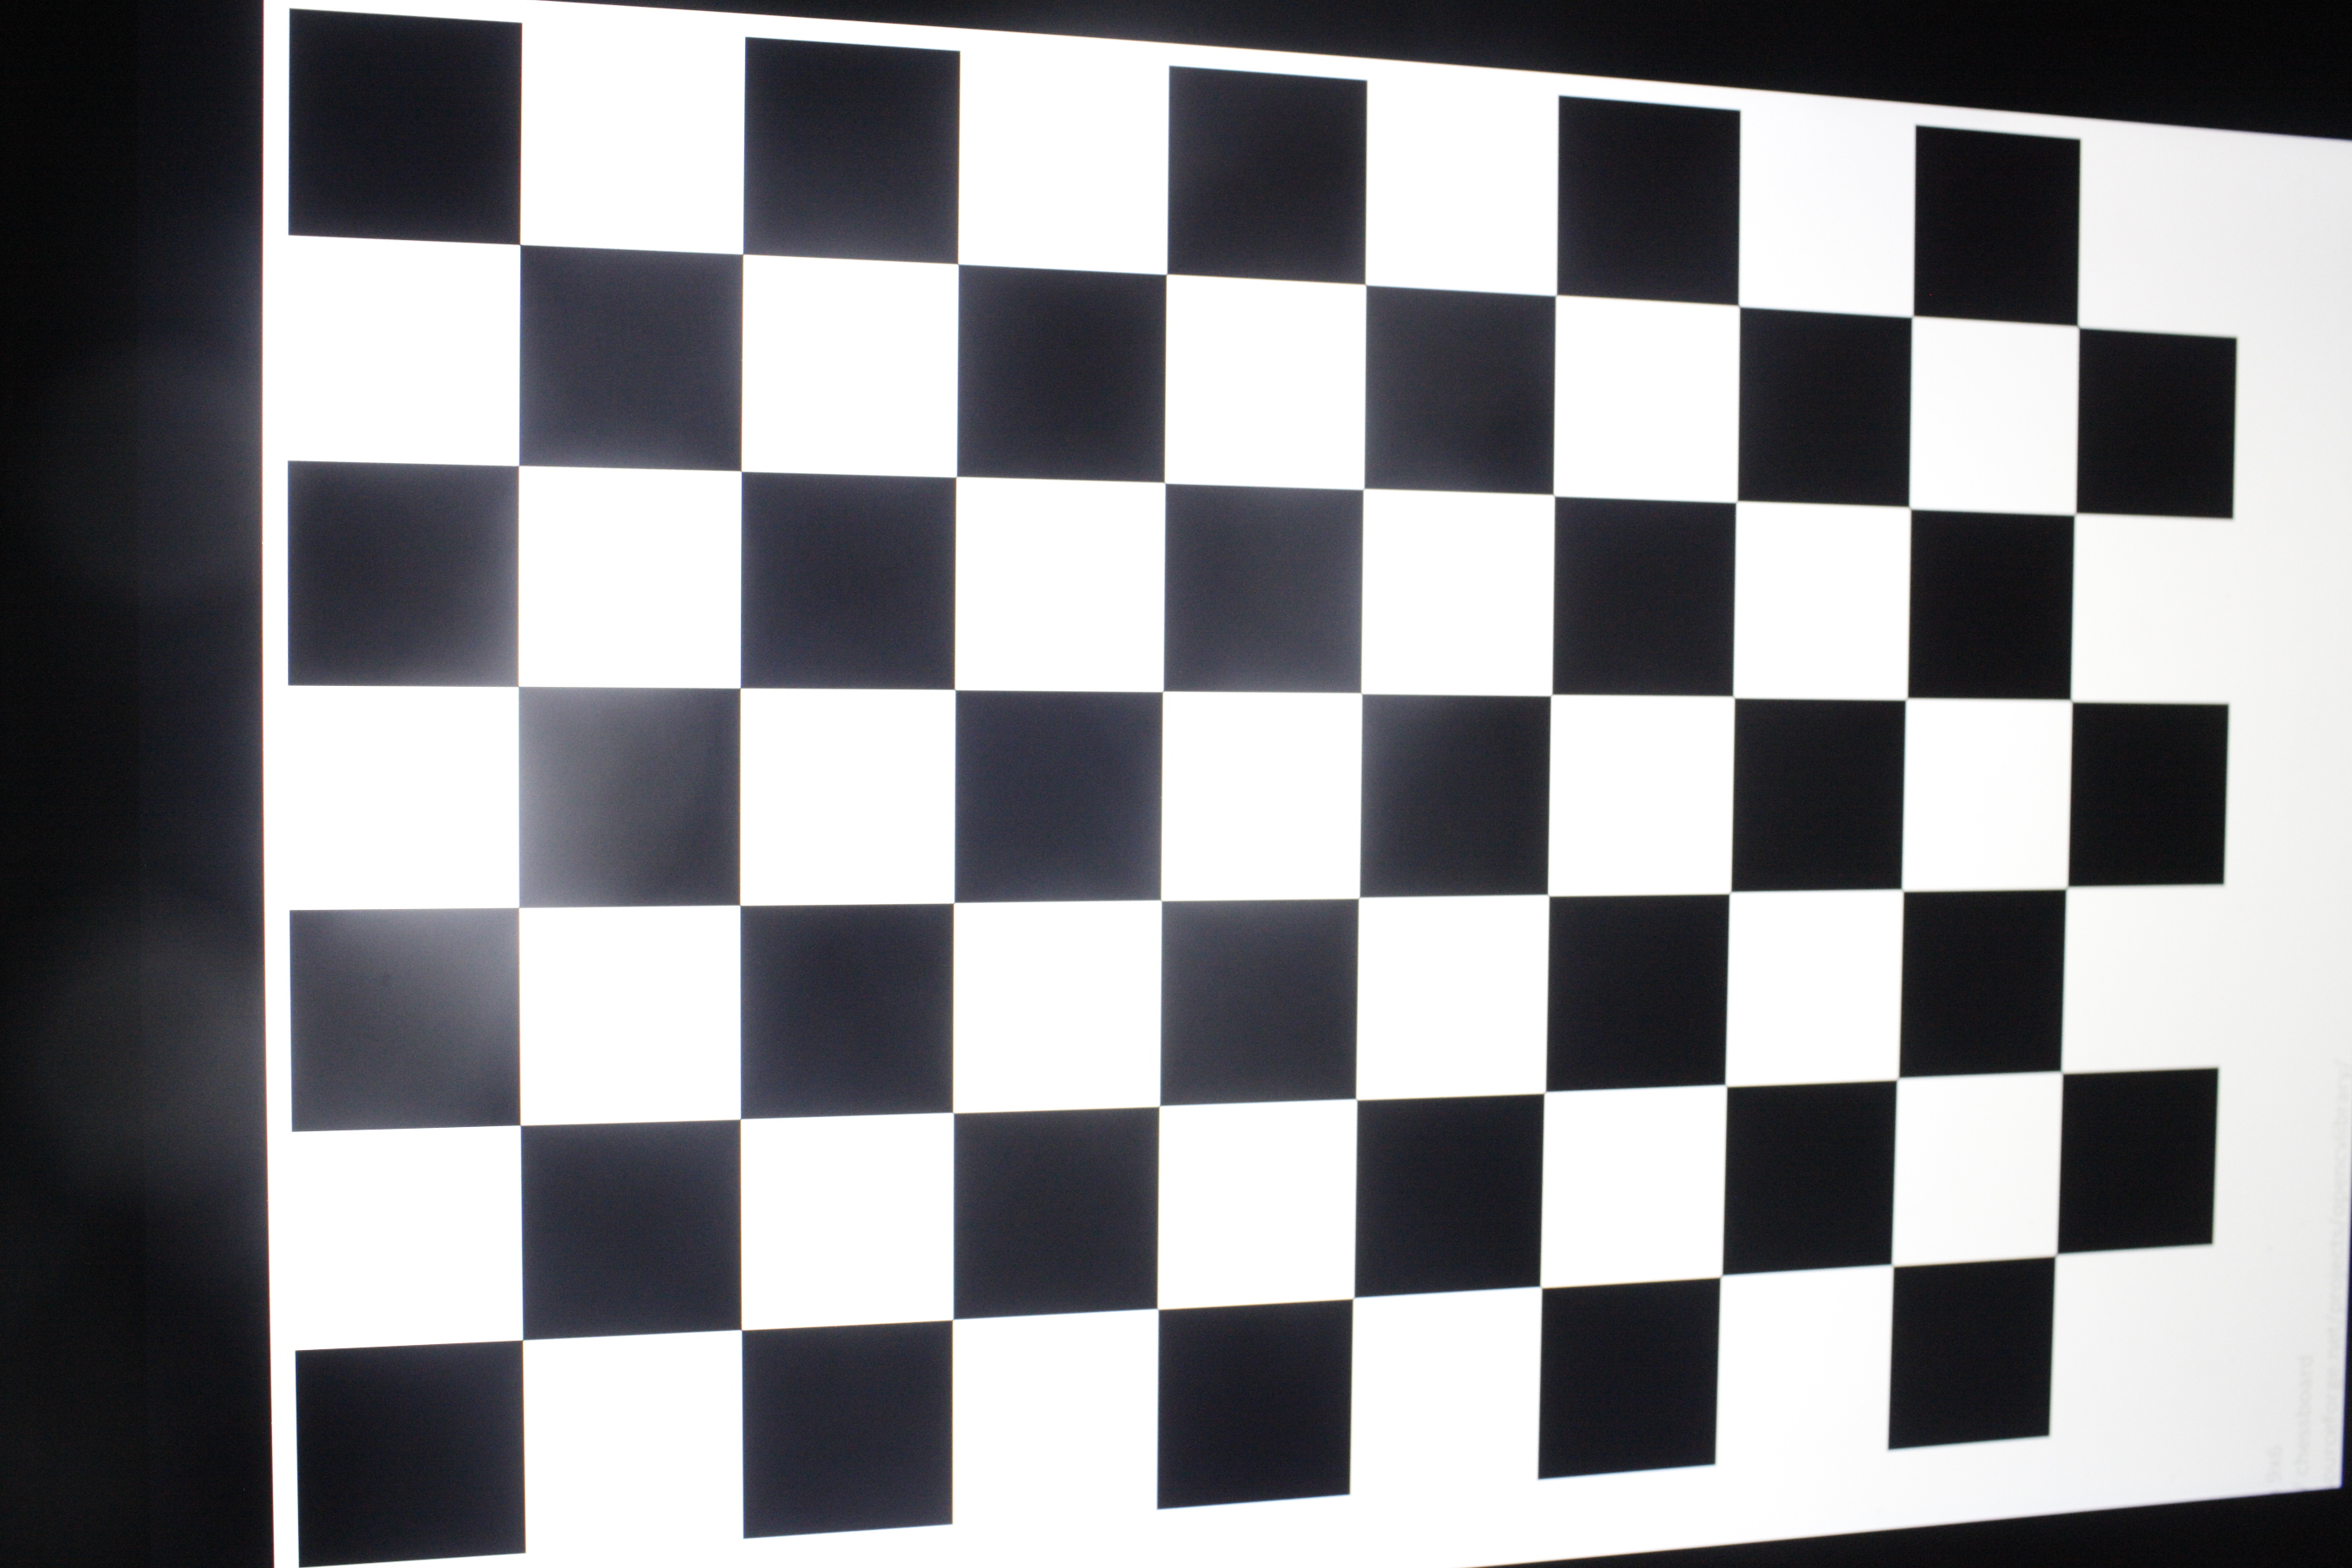
\includegraphics[width=.3\columnwidth]{images/chessboard/p2}
}
\subfigure[Image 3]{
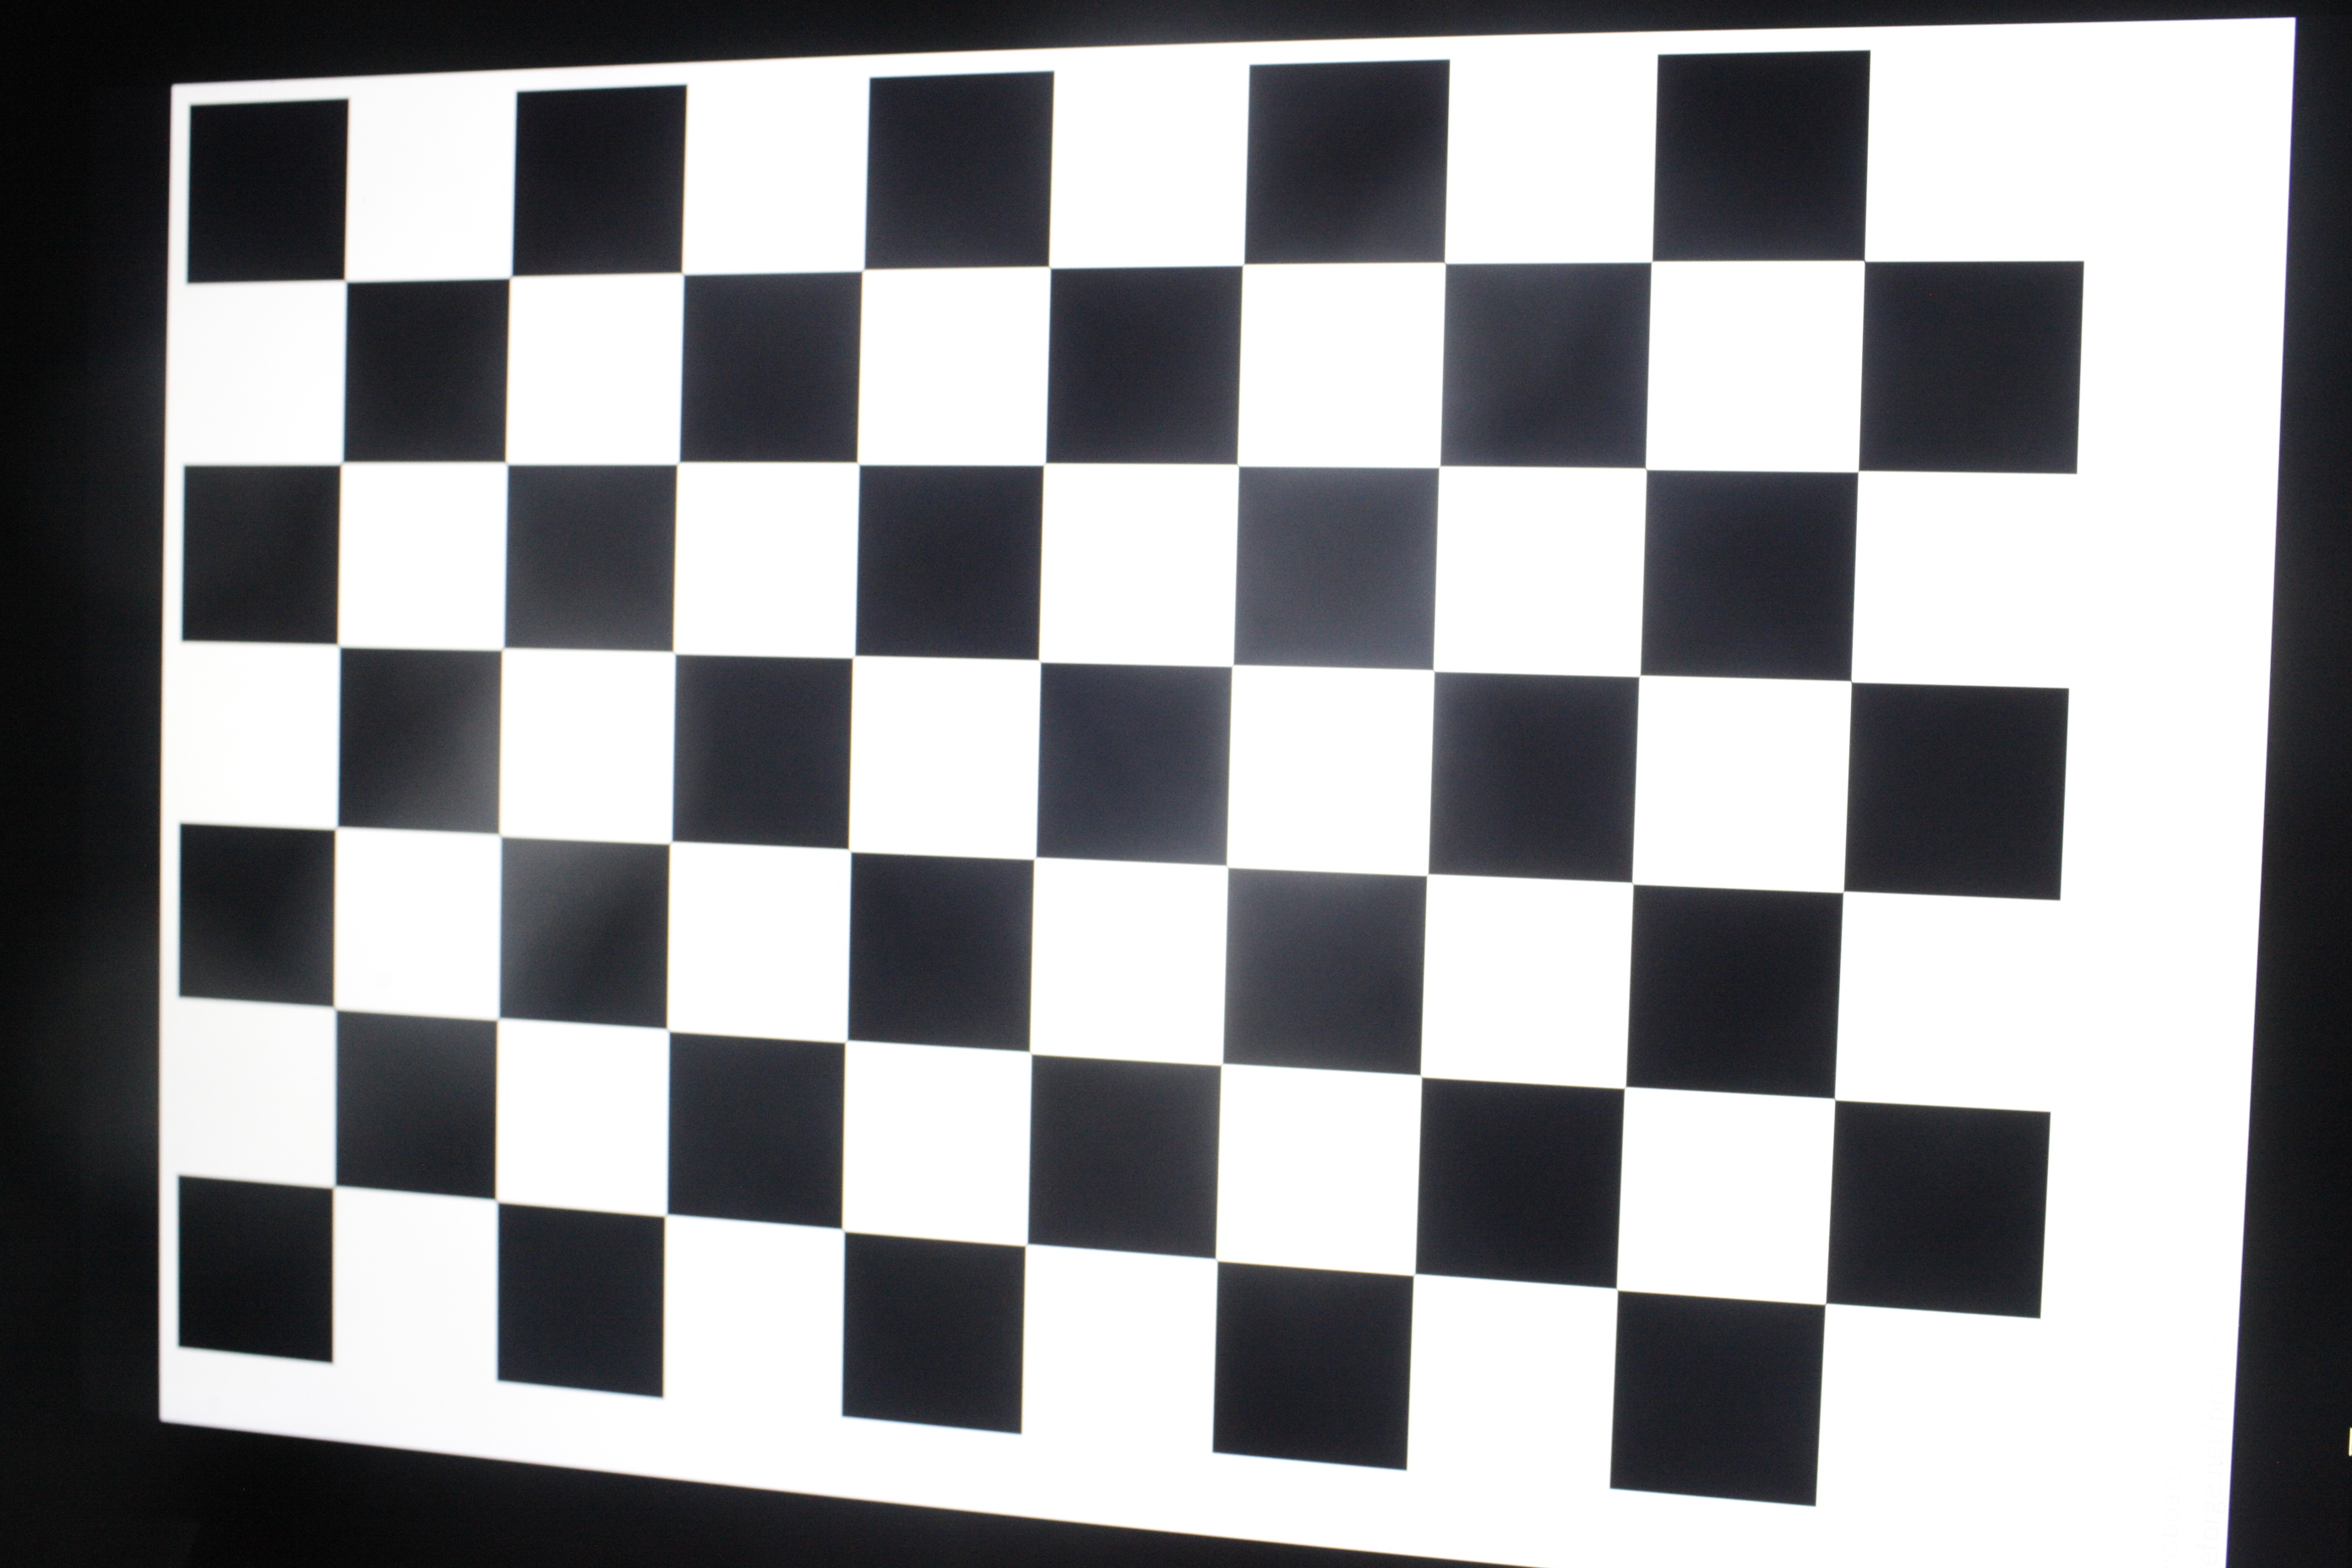
\includegraphics[width=.3\columnwidth]{images/chessboard/p3}
}
\subfigure[Image 4]{
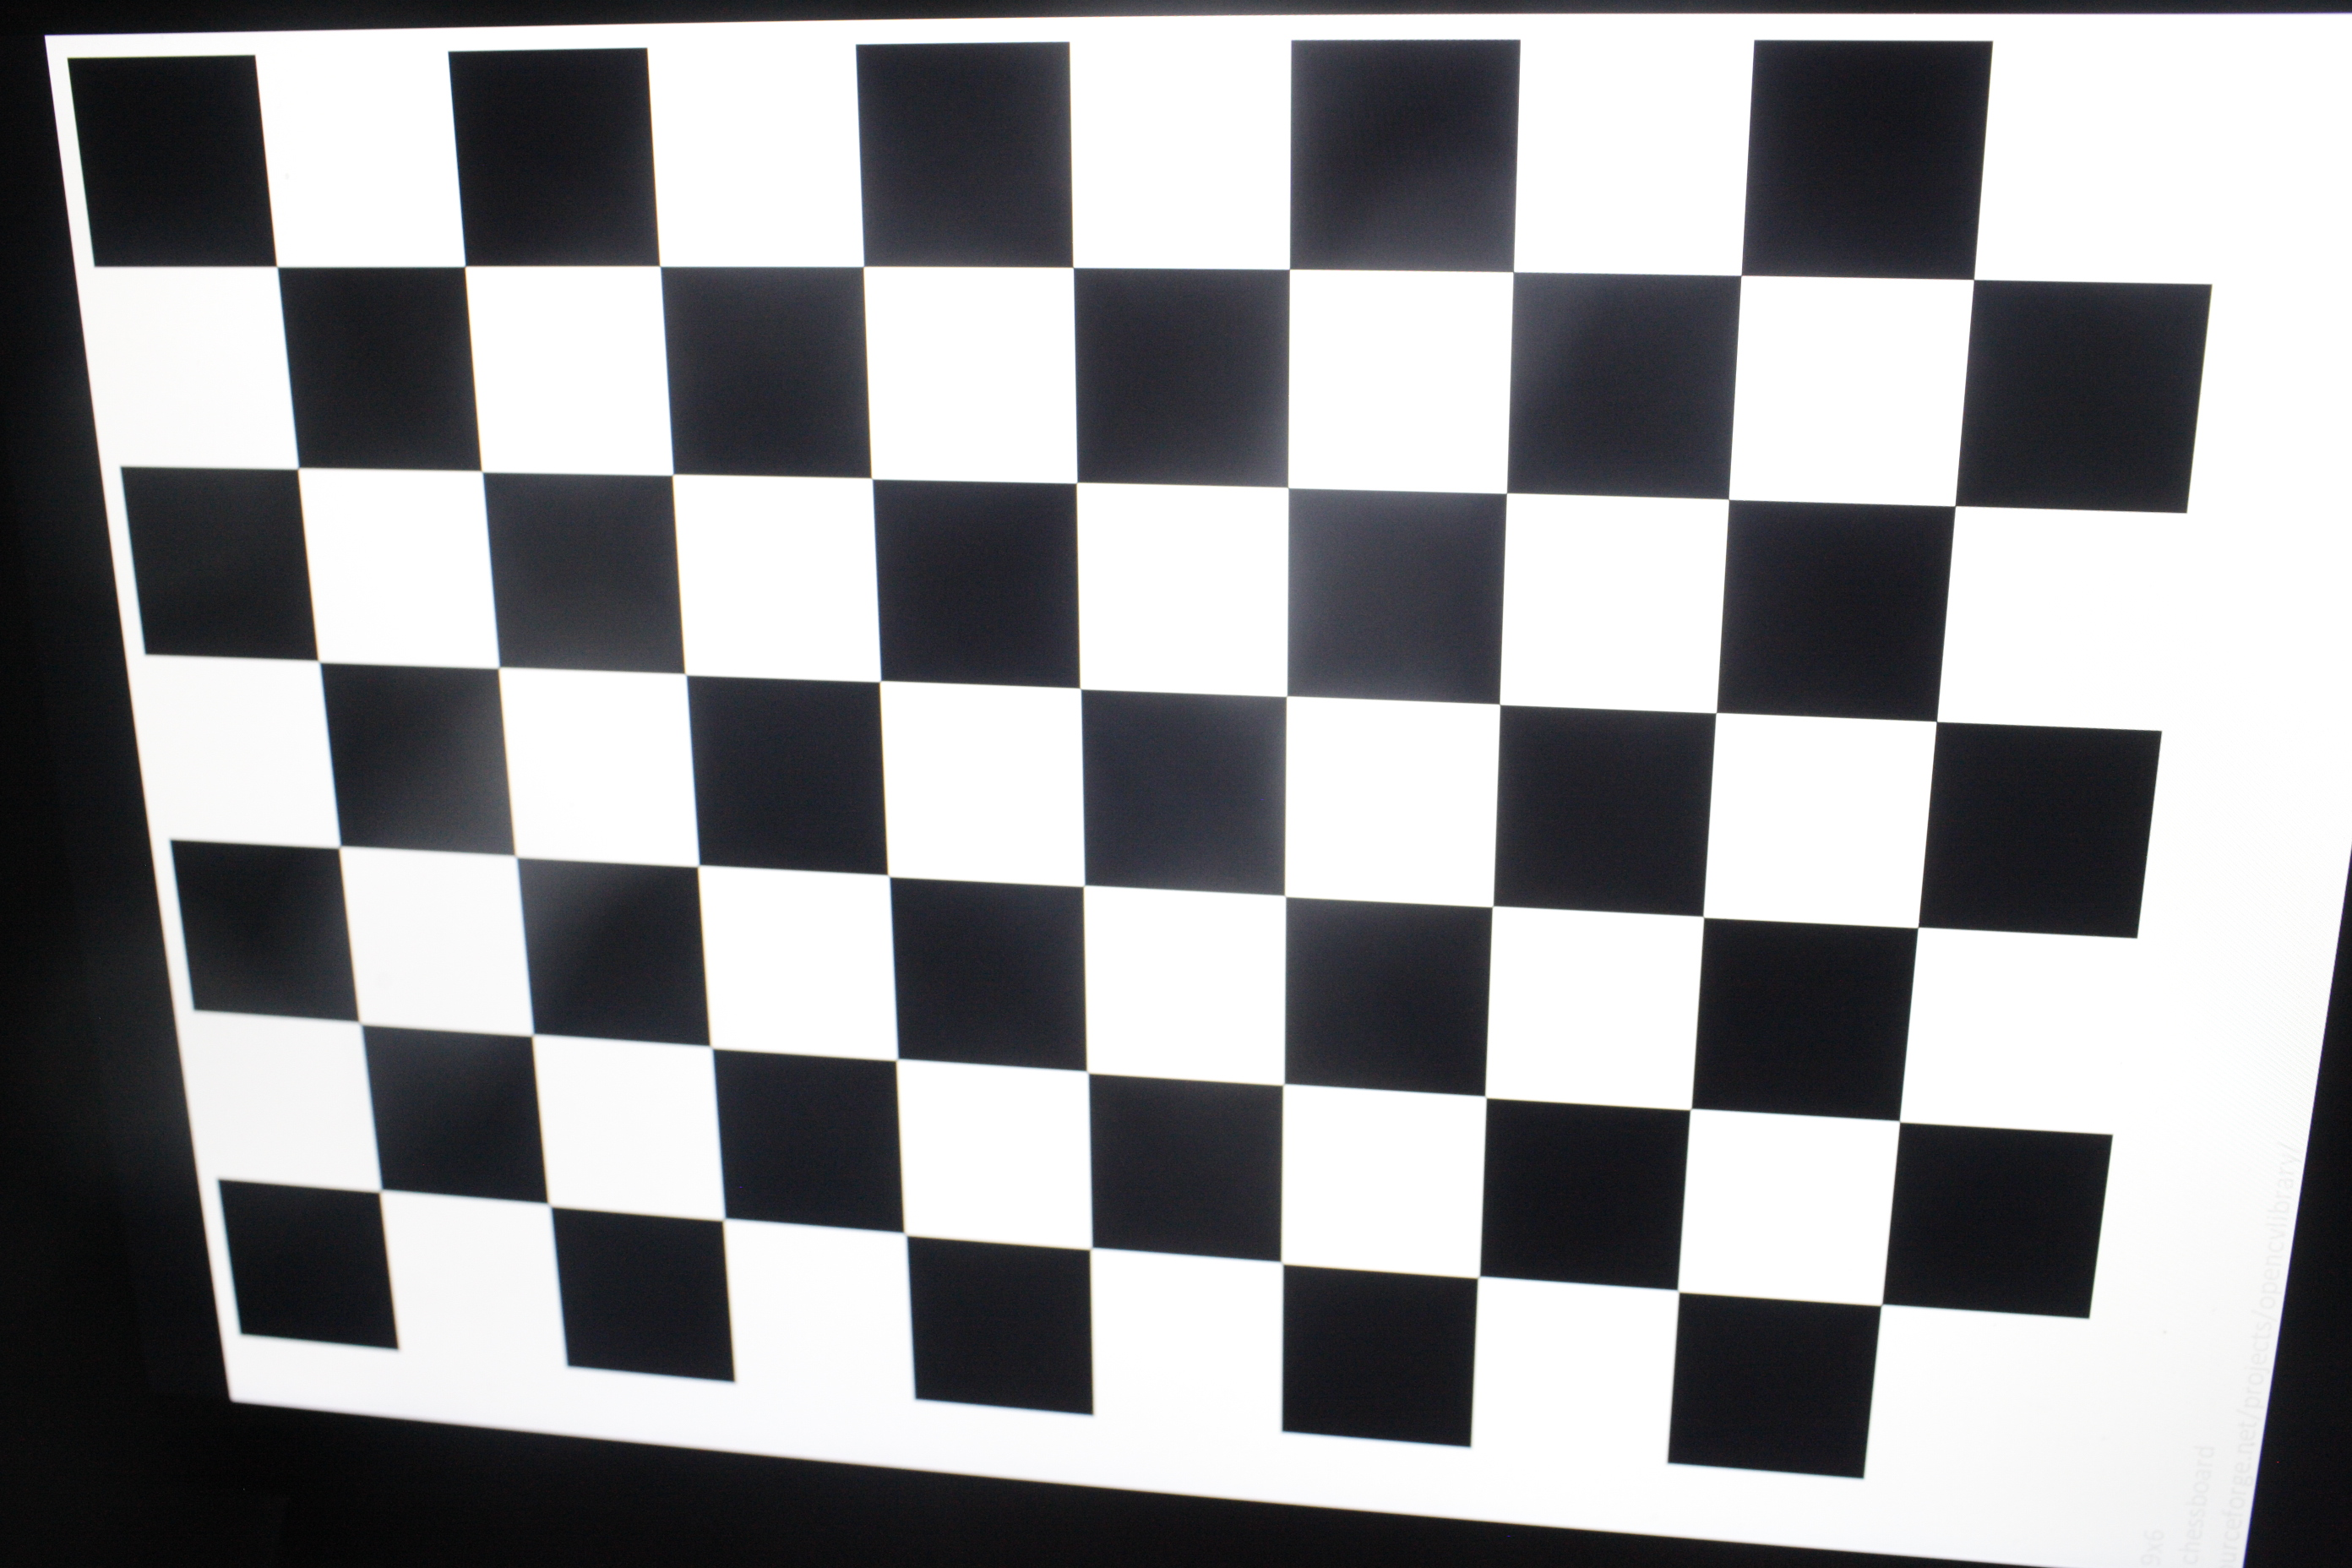
\includegraphics[width=.3\columnwidth]{images/chessboard/p4}
}
\subfigure[Image 5]{
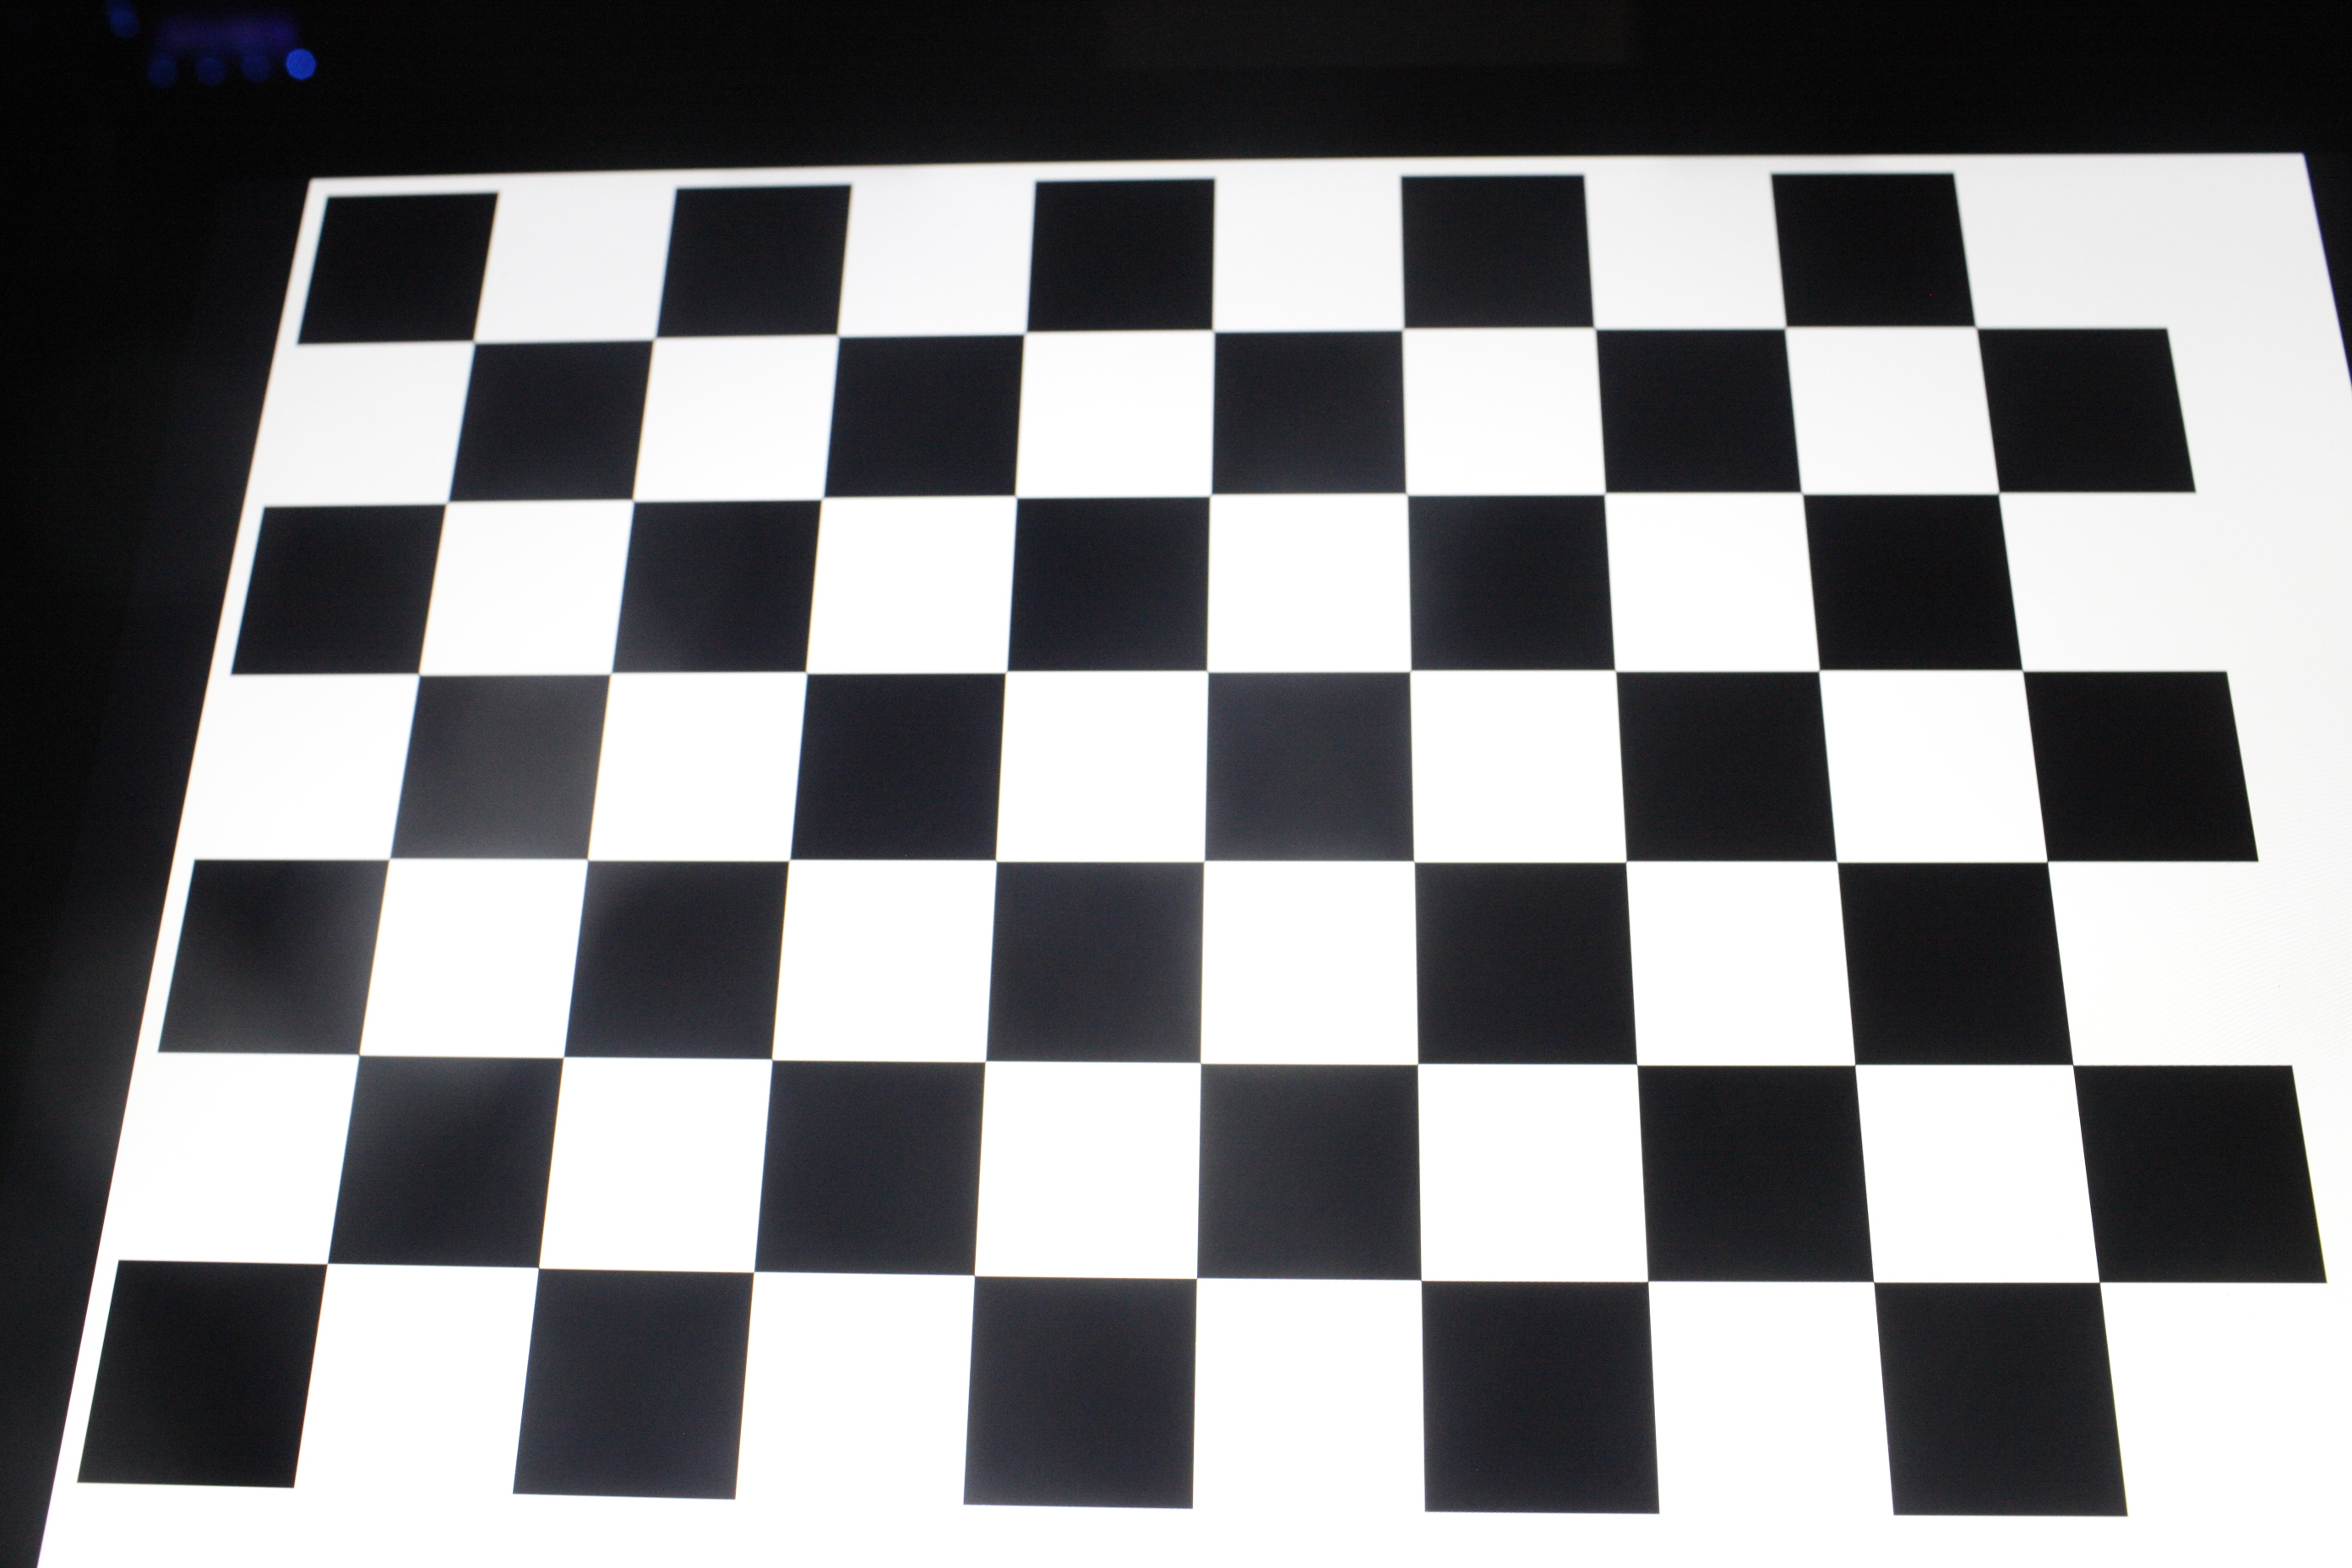
\includegraphics[width=.3\columnwidth]{images/chessboard/p5}
}
\subfigure[Image 6]{
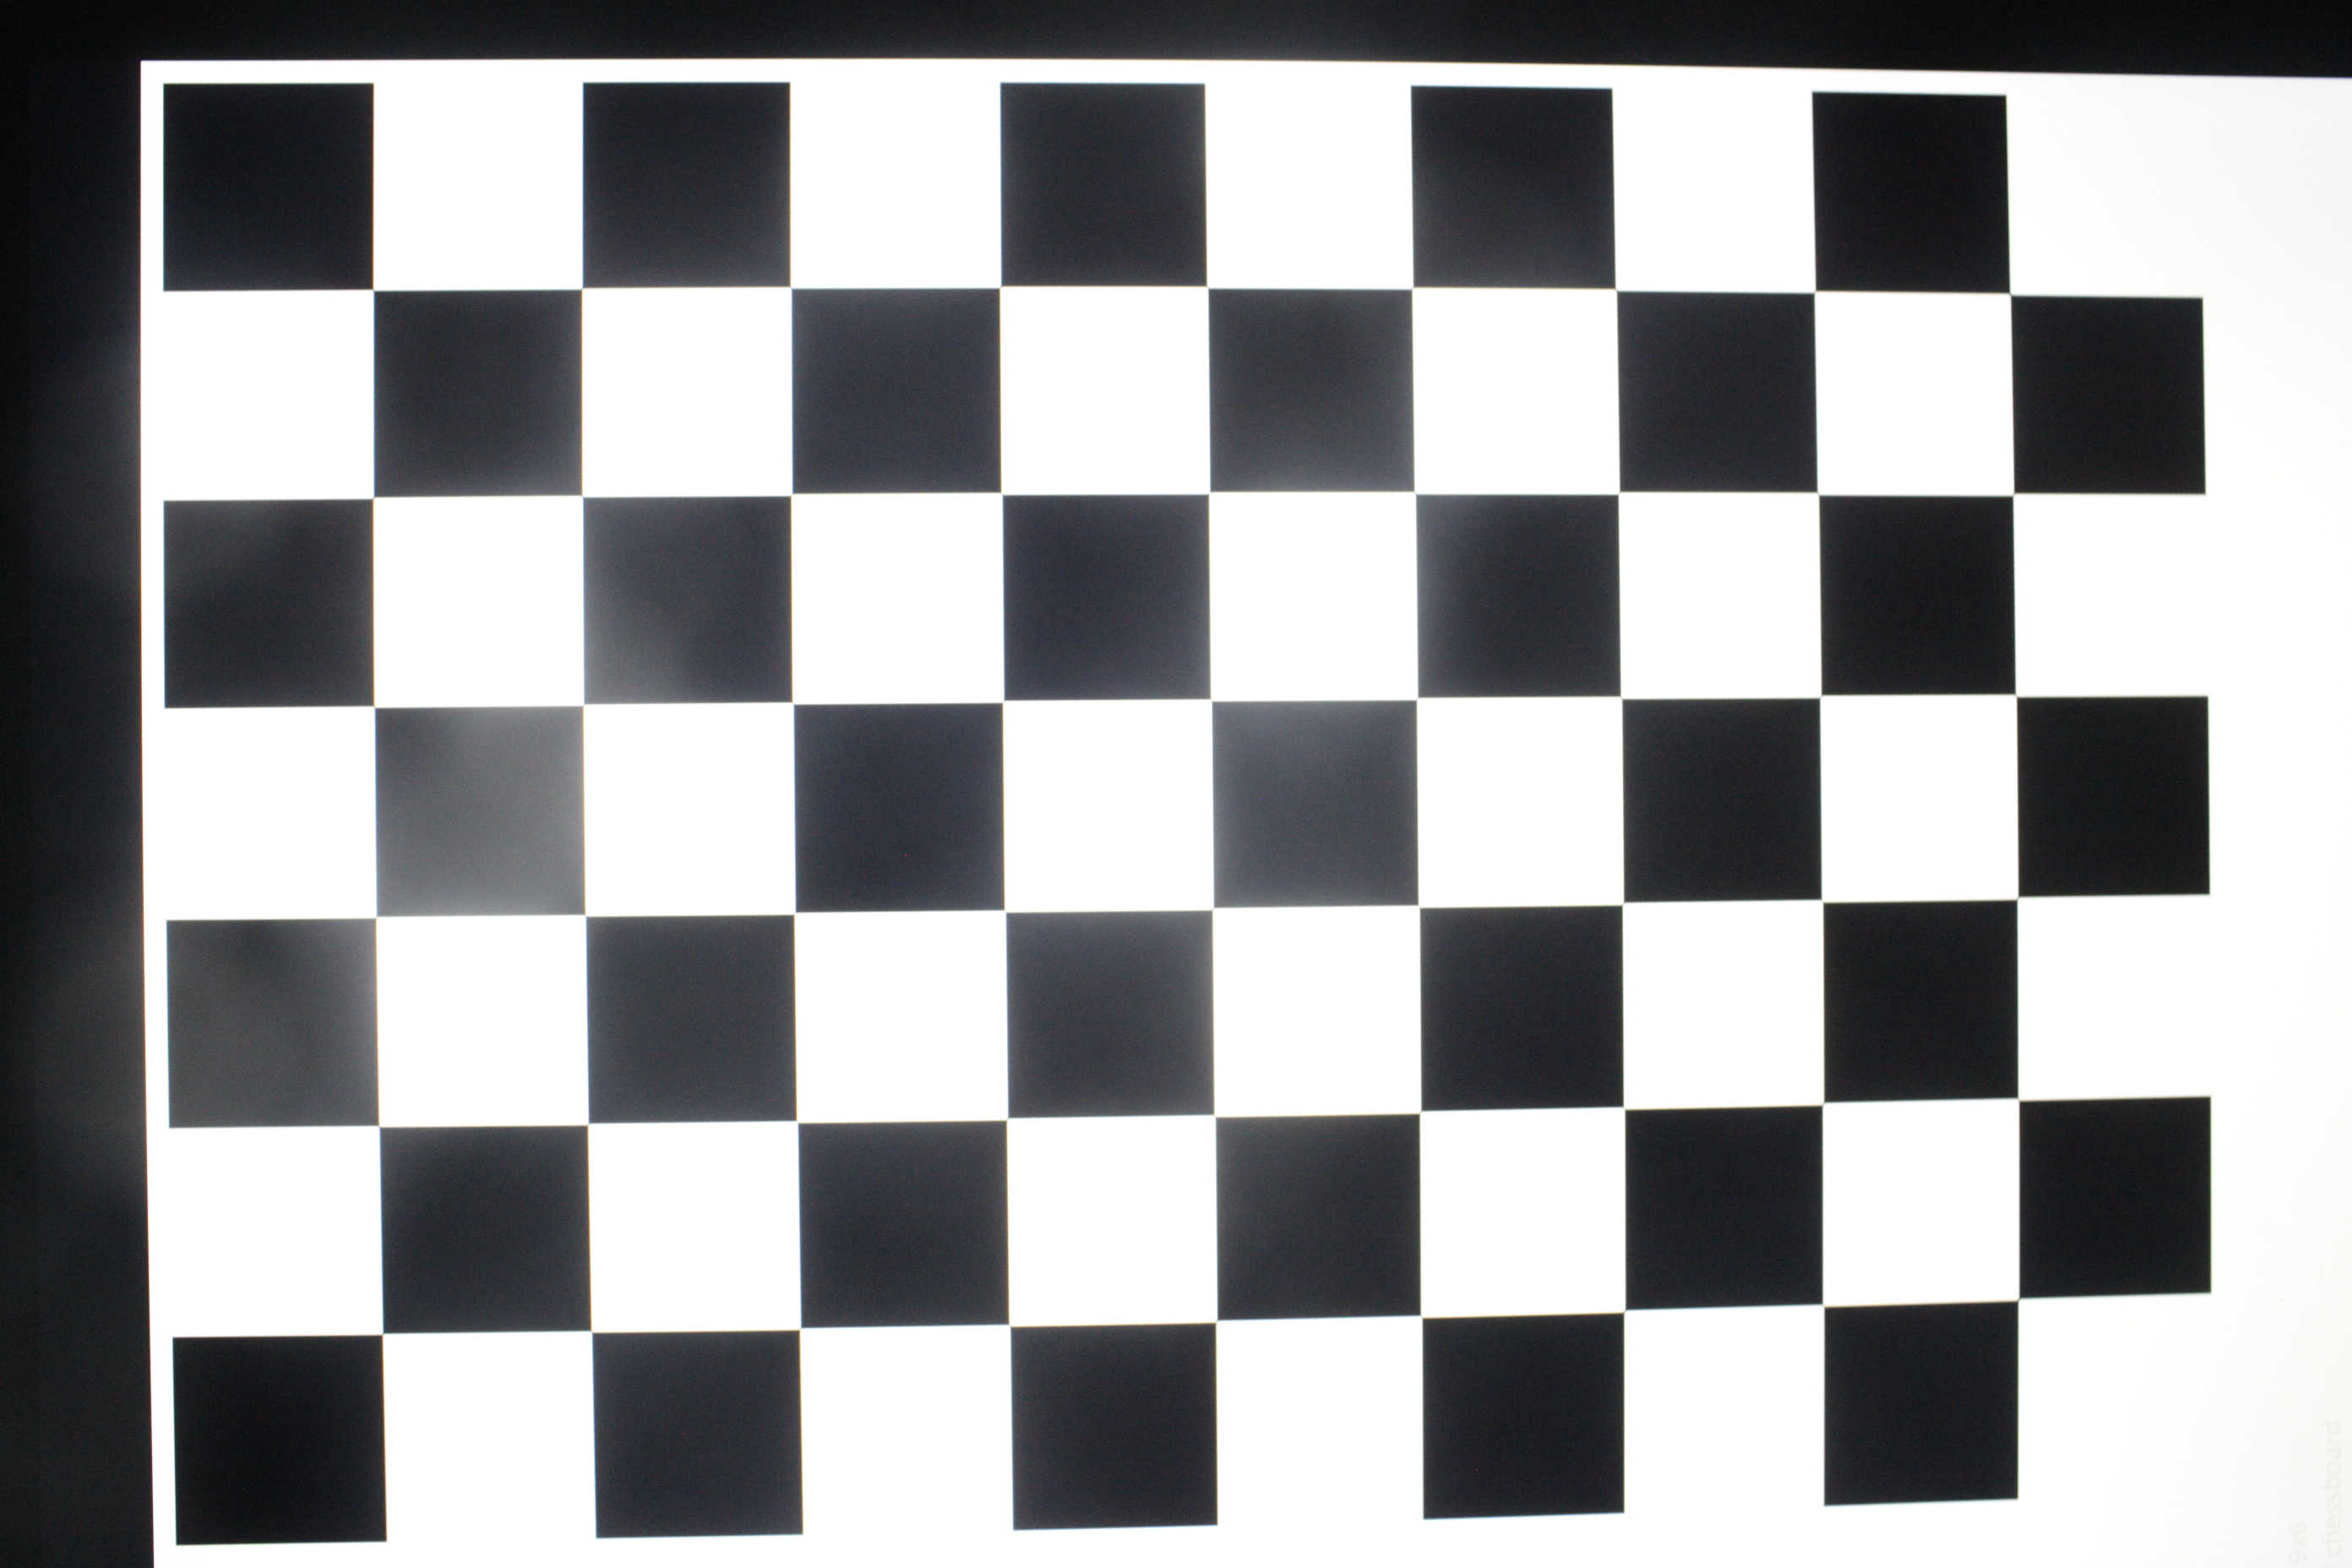
\includegraphics[width=.3\columnwidth]{images/chessboard/p6}
}
\subfigure[Image 7]{
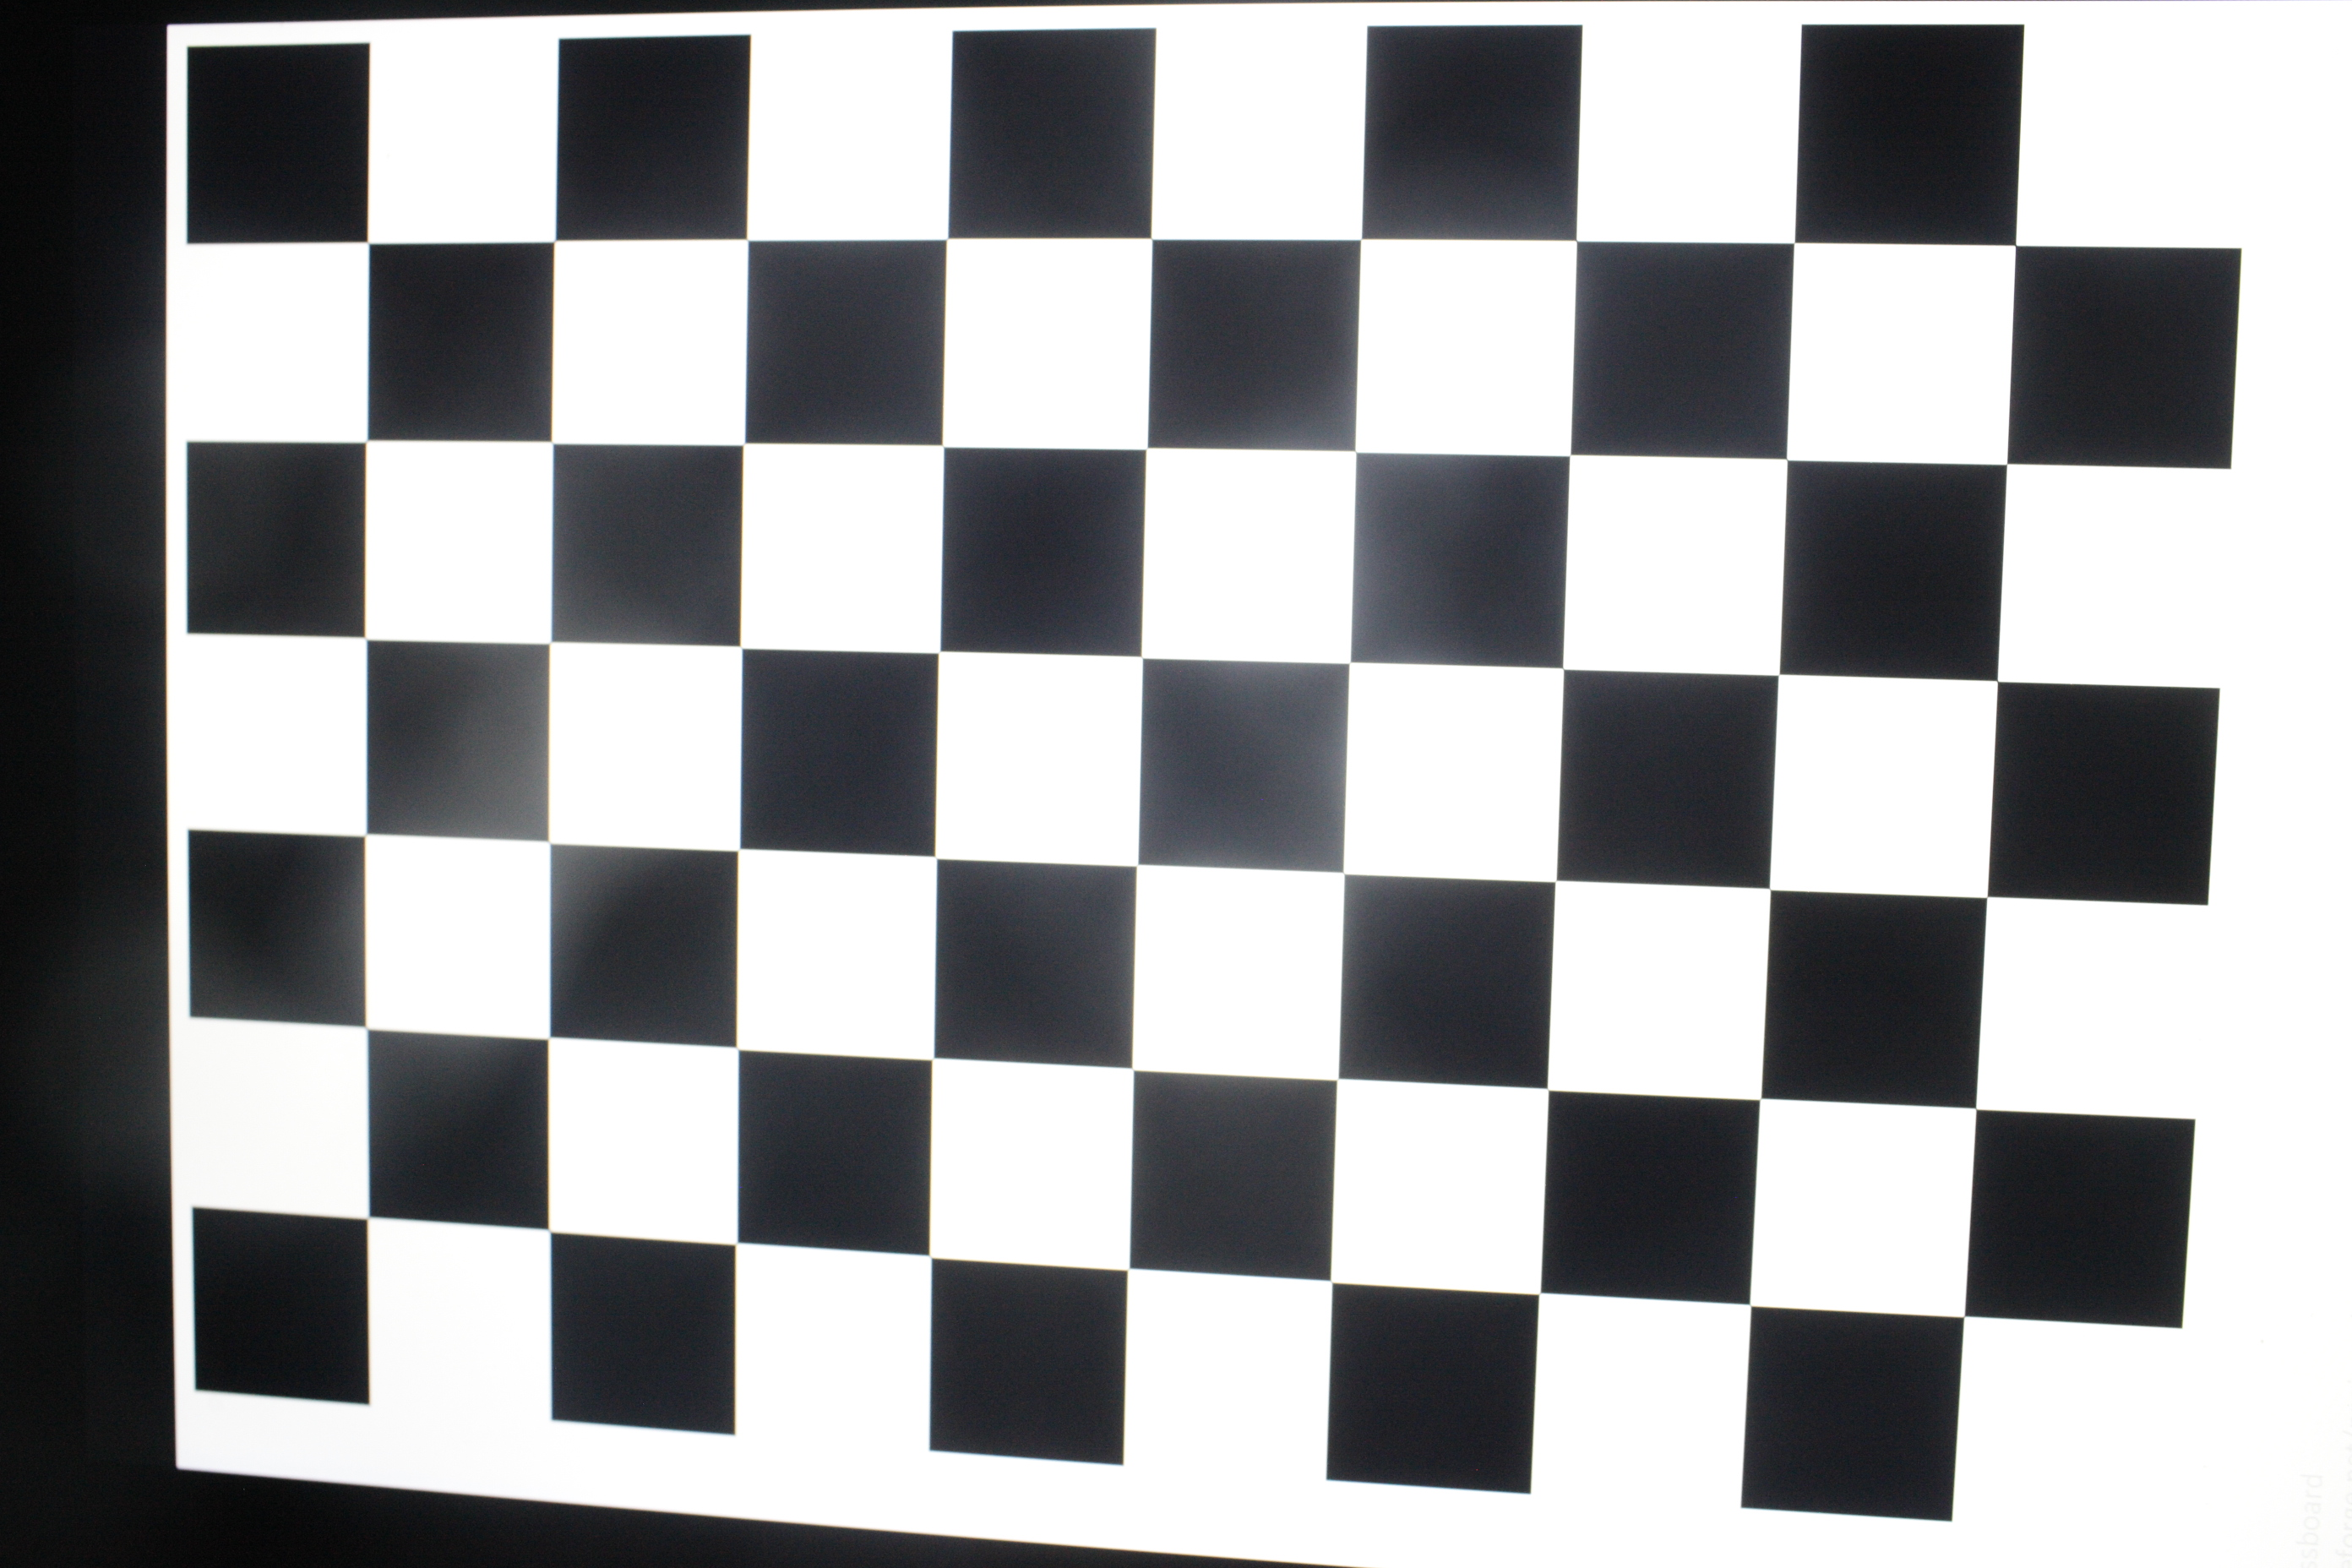
\includegraphics[width=.3\columnwidth]{images/chessboard/p7}
}
\subfigure[Image 8]{
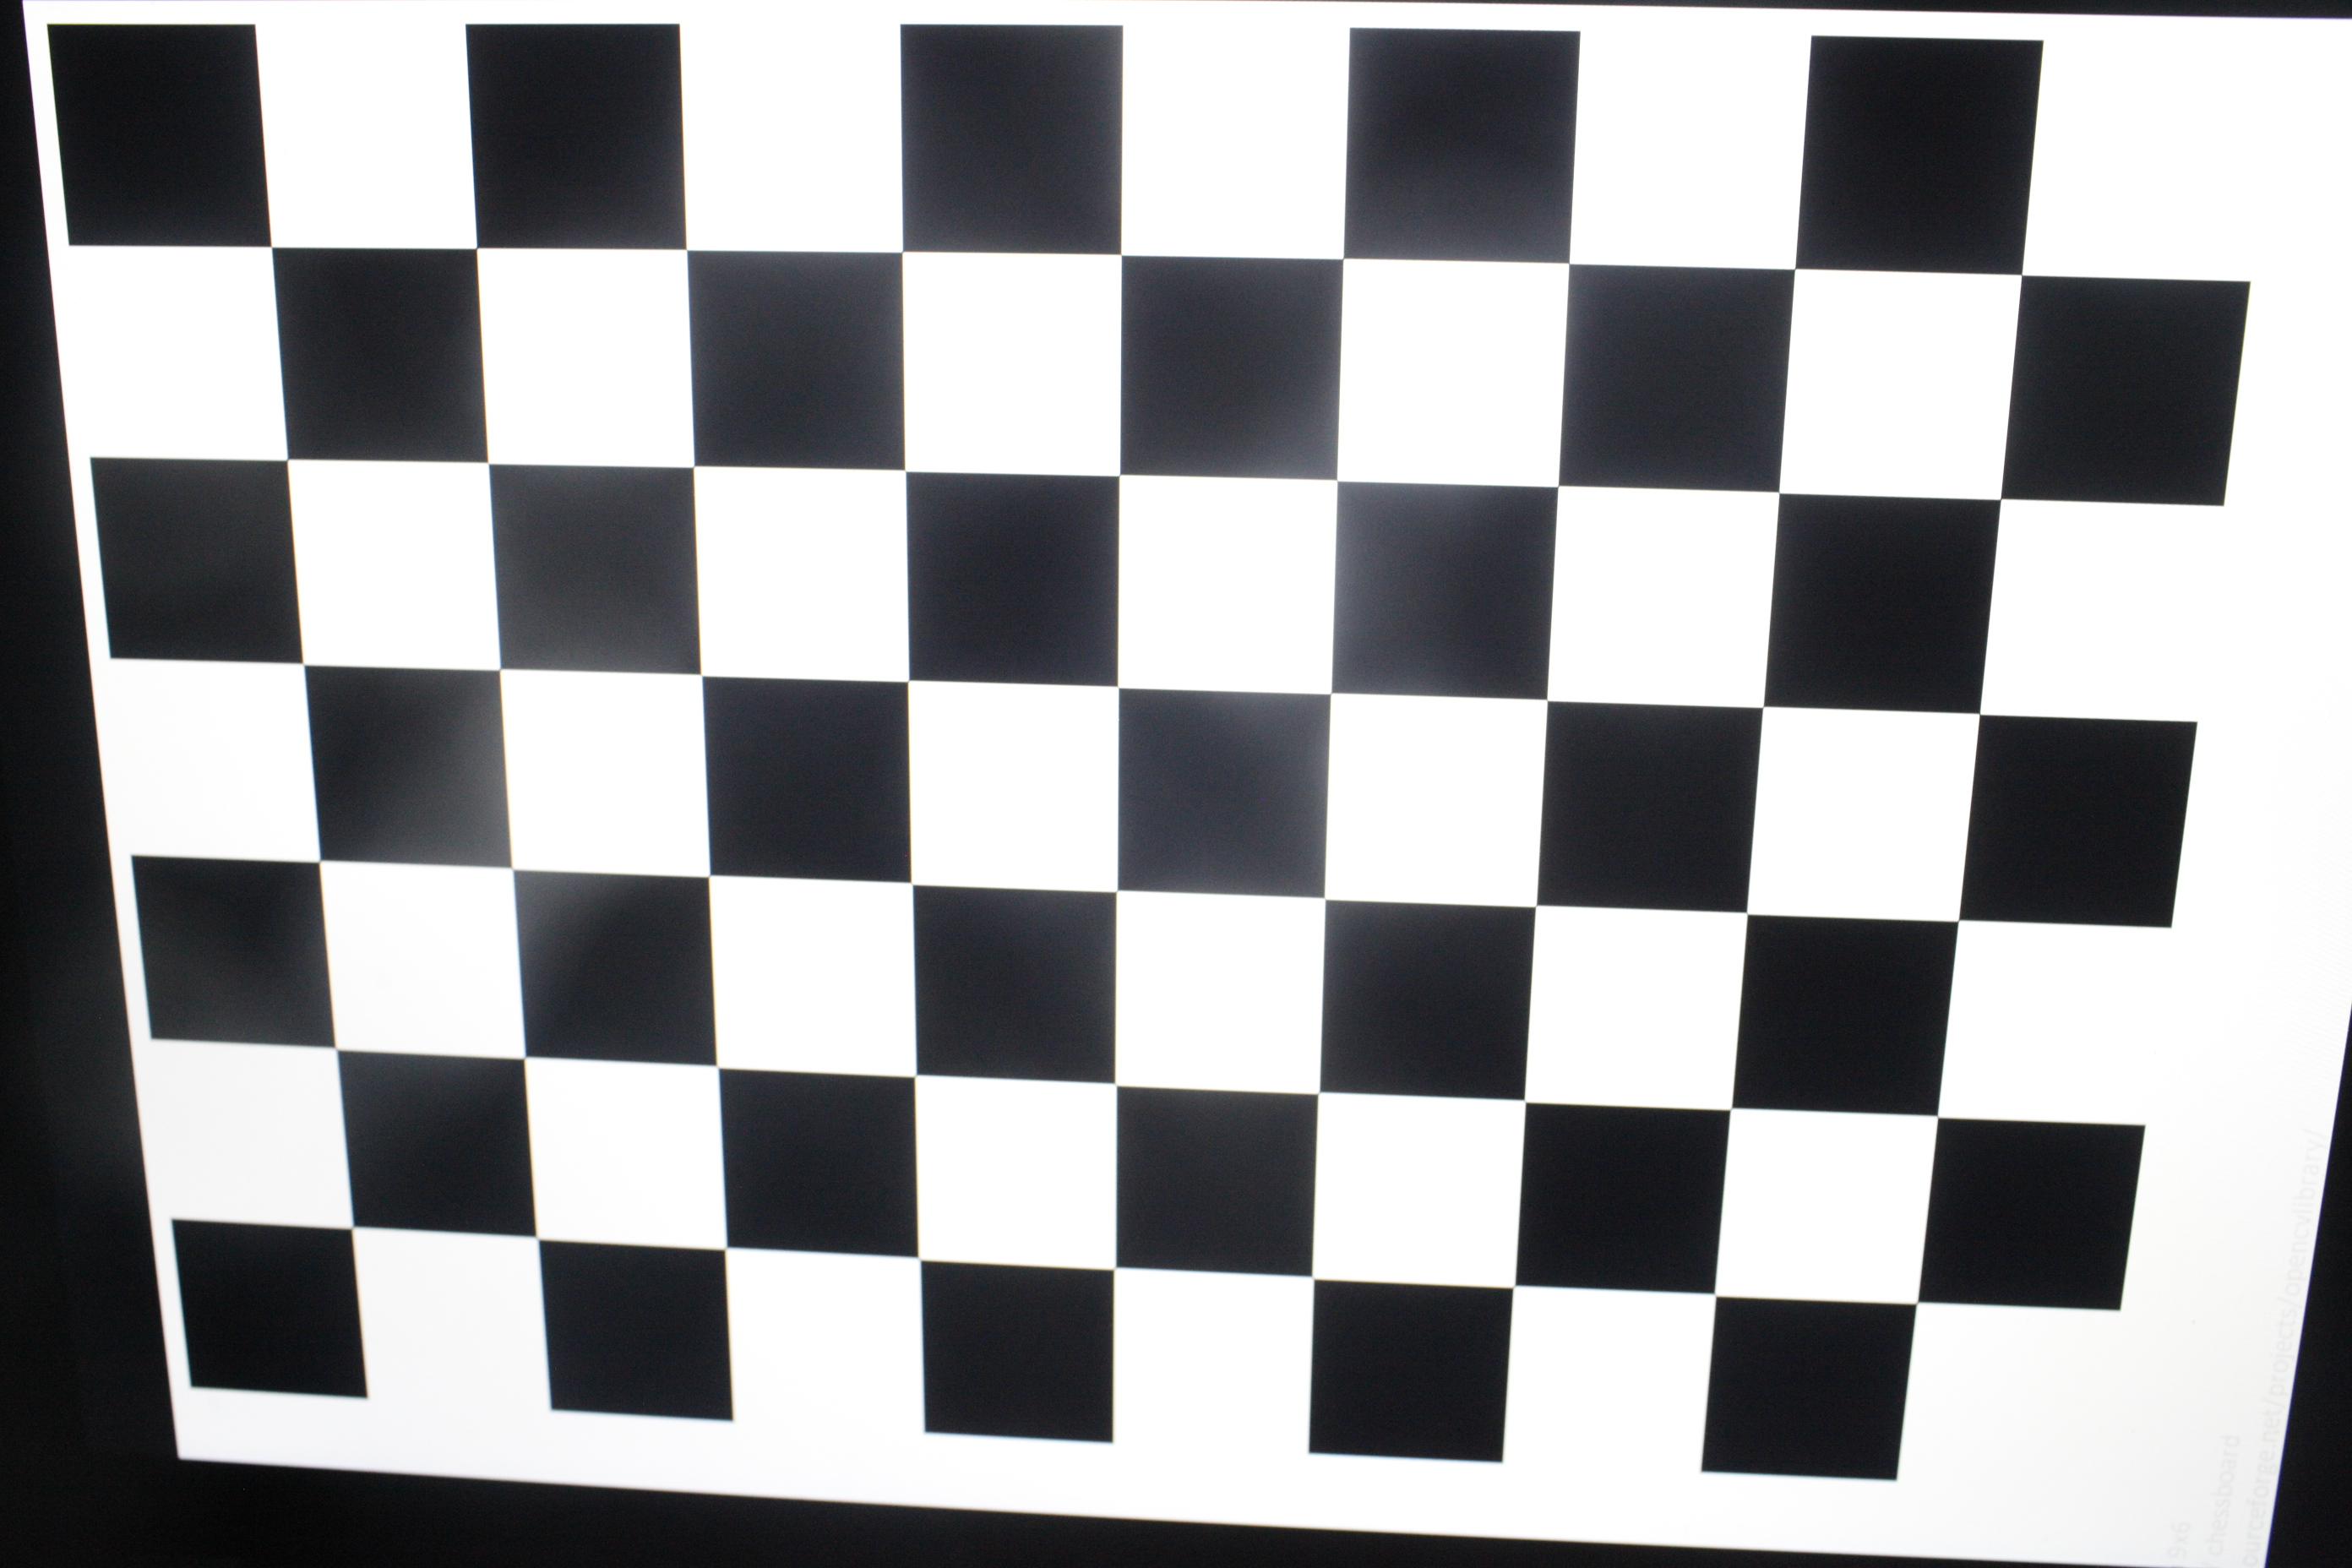
\includegraphics[width=.3\columnwidth]{images/chessboard/p8}
}
\subfigure[Image 9]{
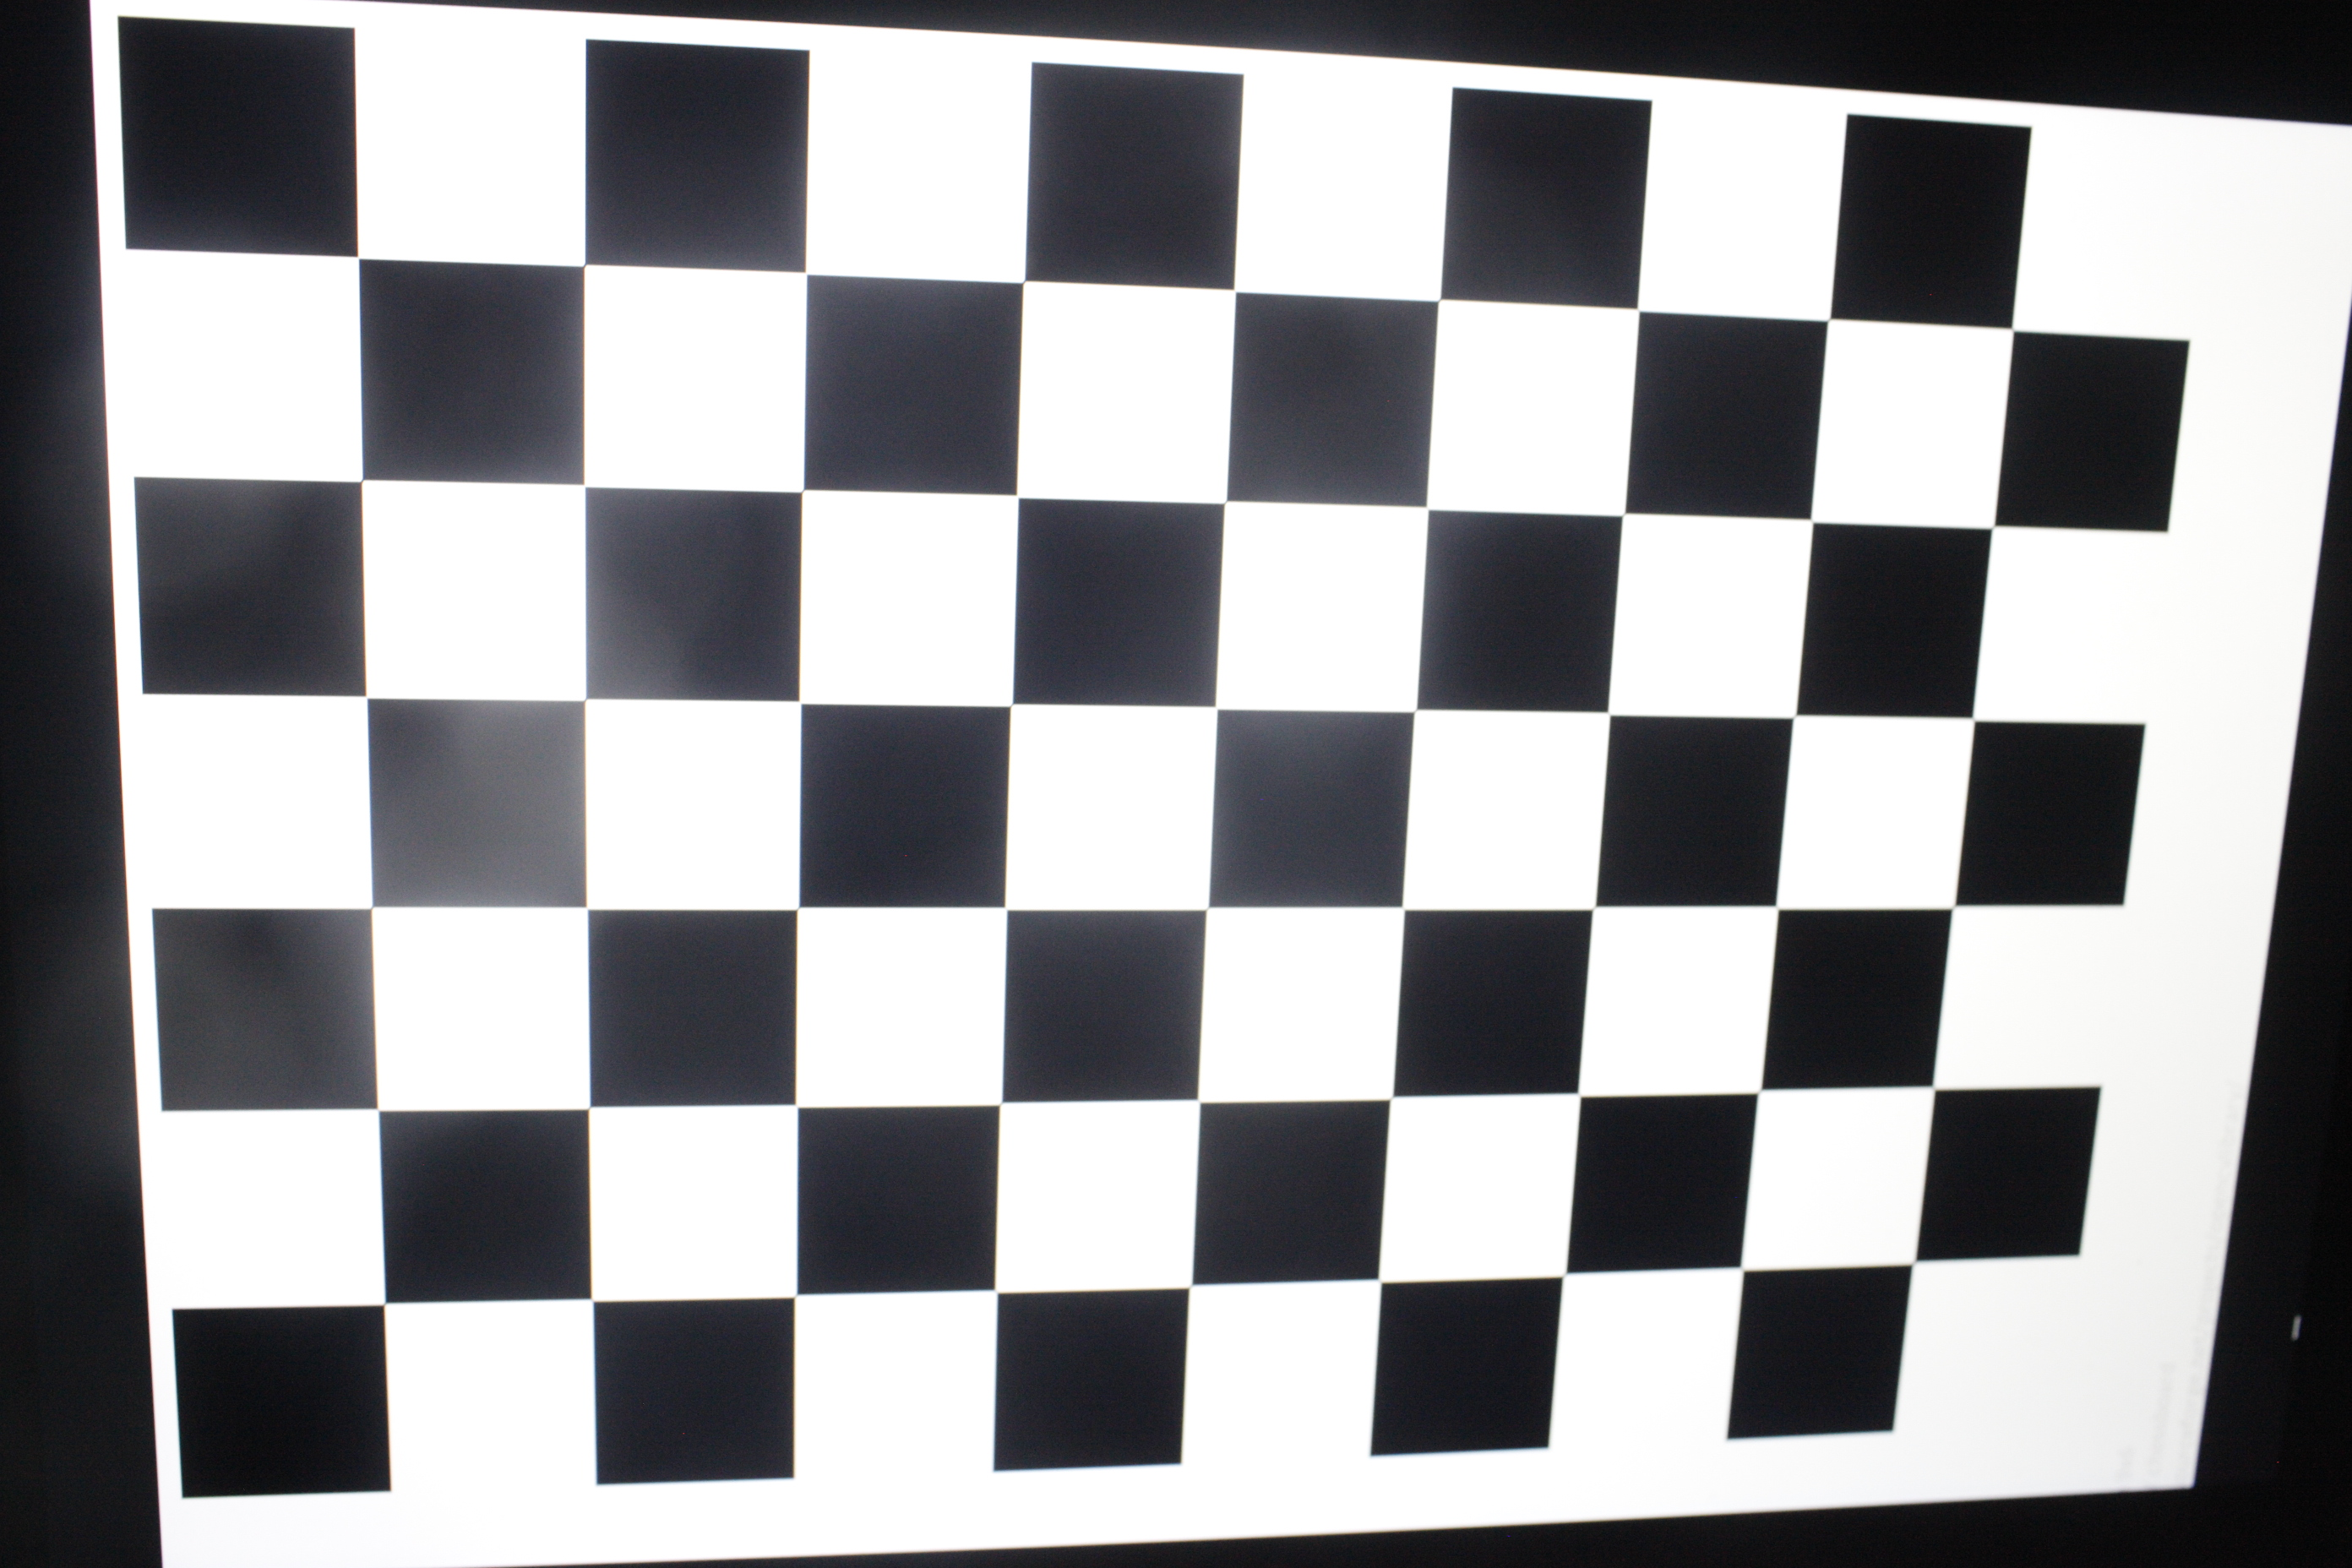
\includegraphics[width=.3\columnwidth]{images/chessboard/p9}
}
\subfigure[Image 10]{
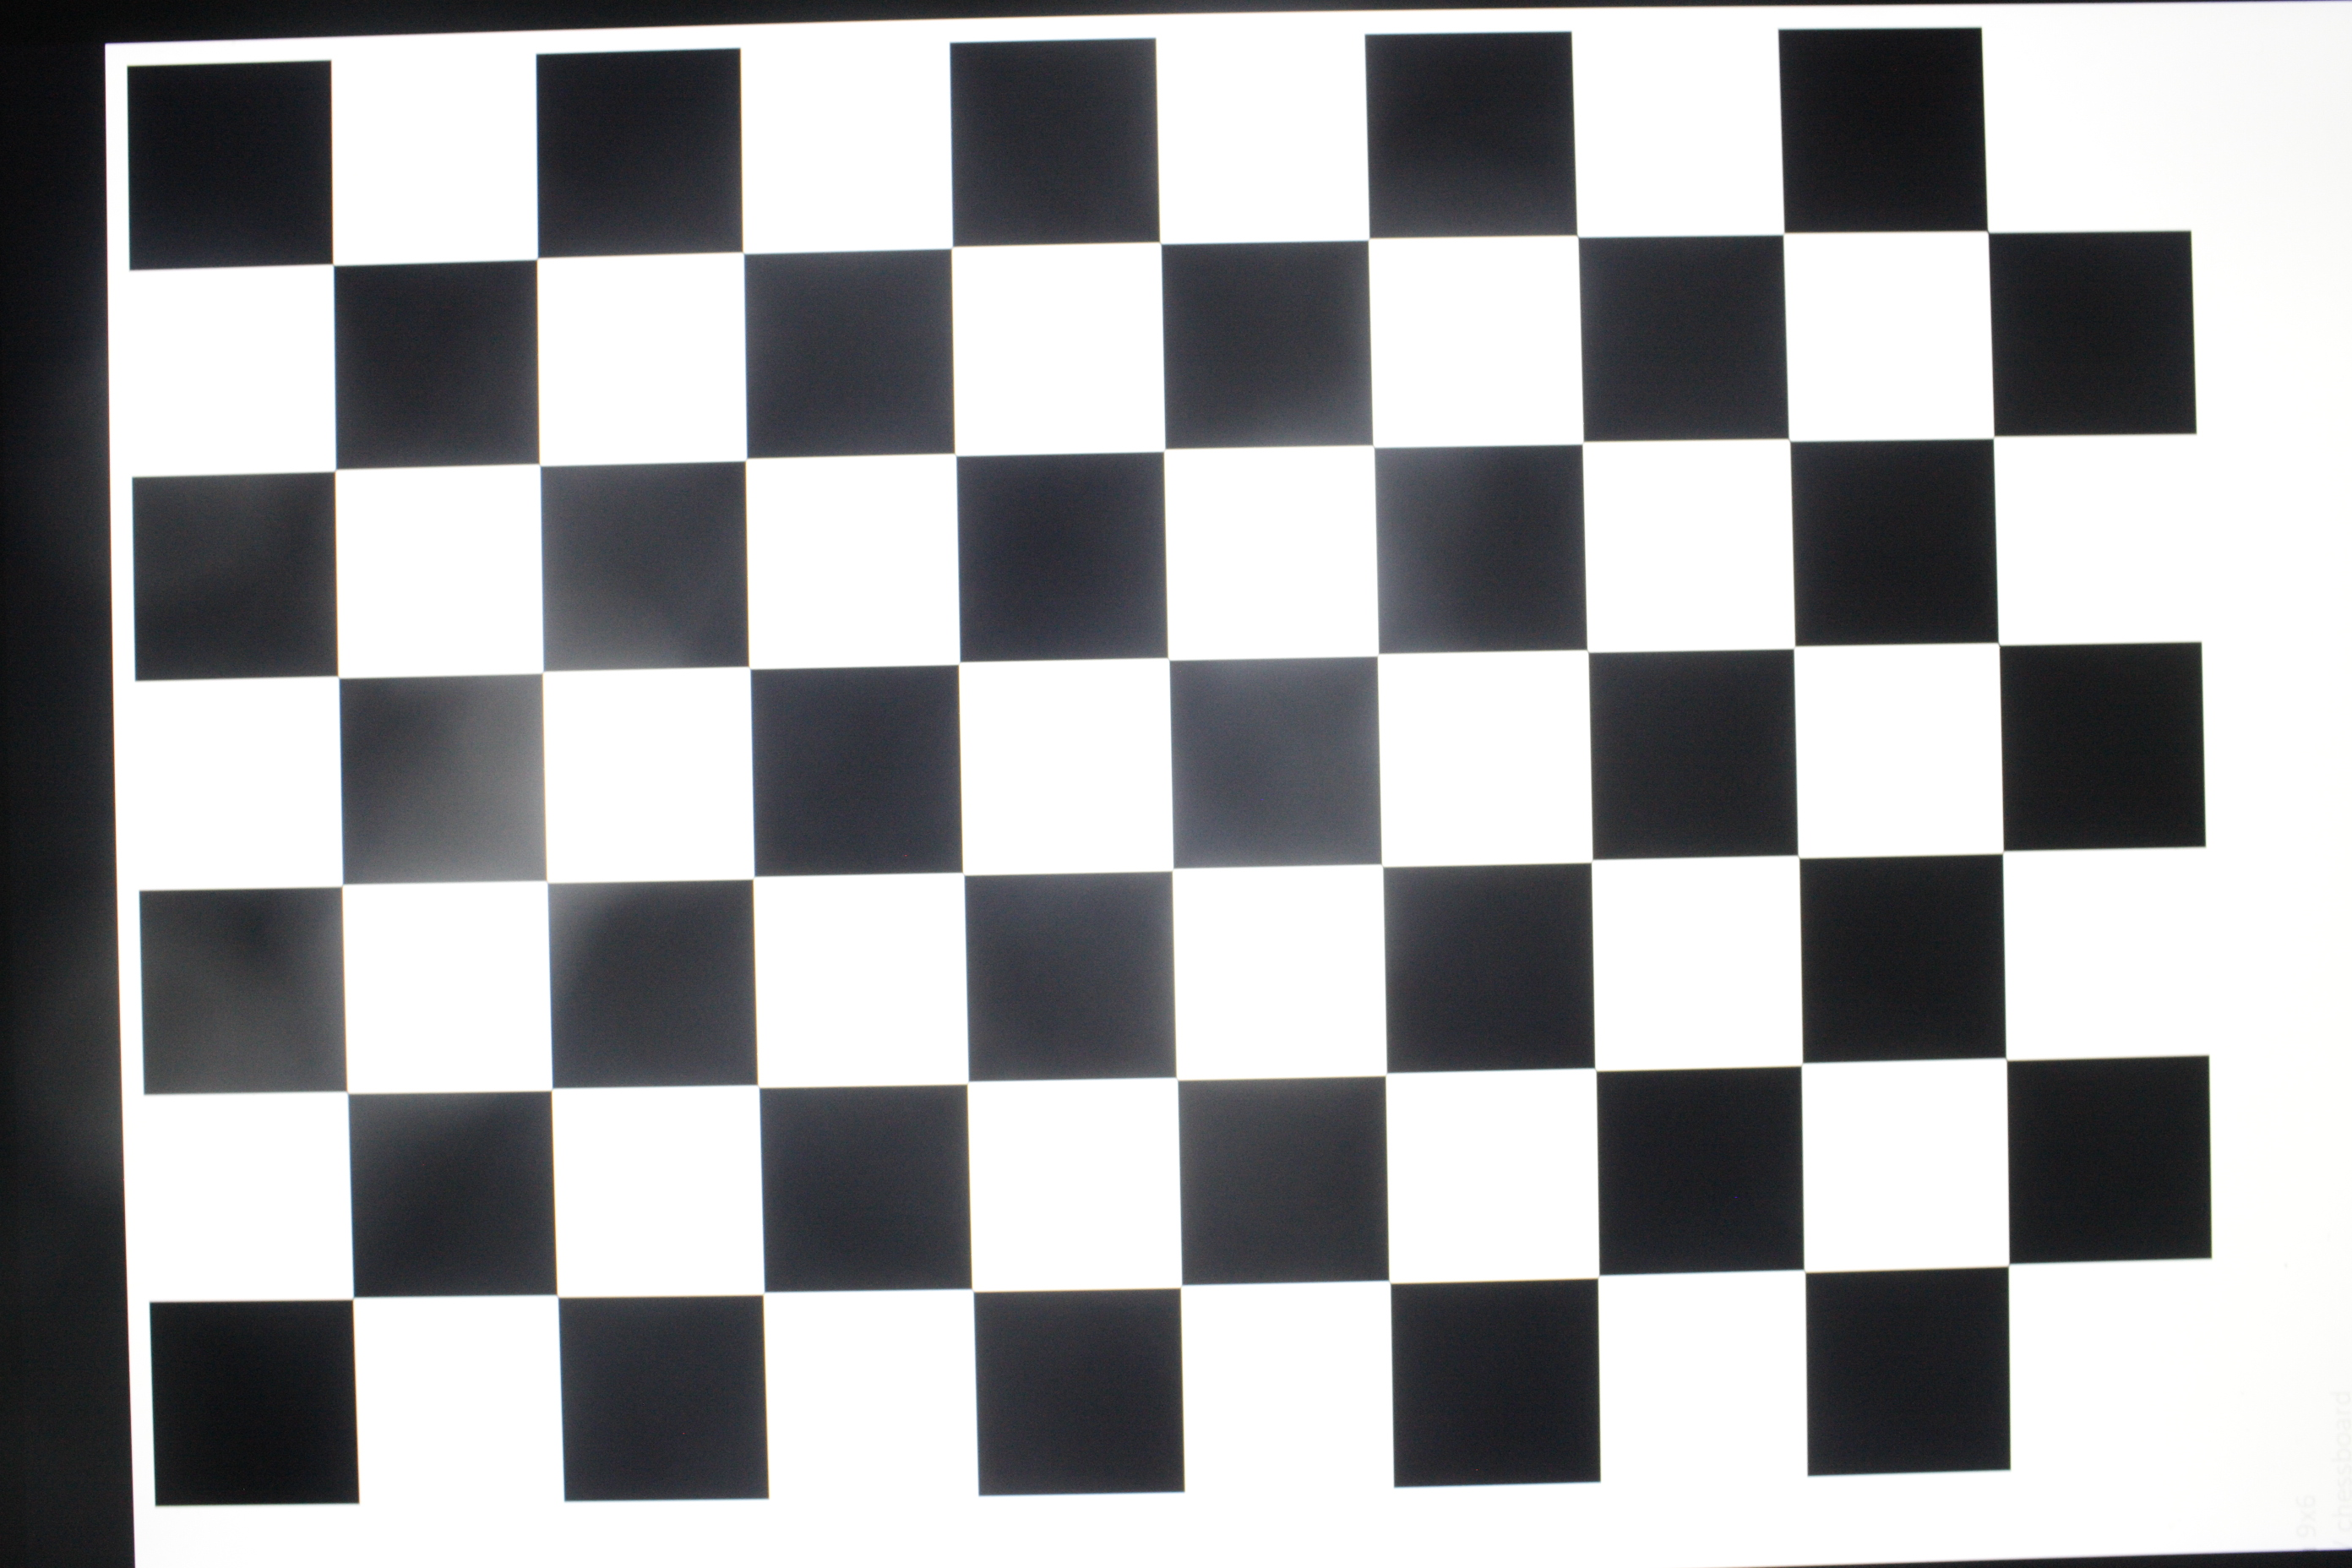
\includegraphics[width=.3\columnwidth]{images/chessboard/p10}
}
\subfigure[Image 11]{
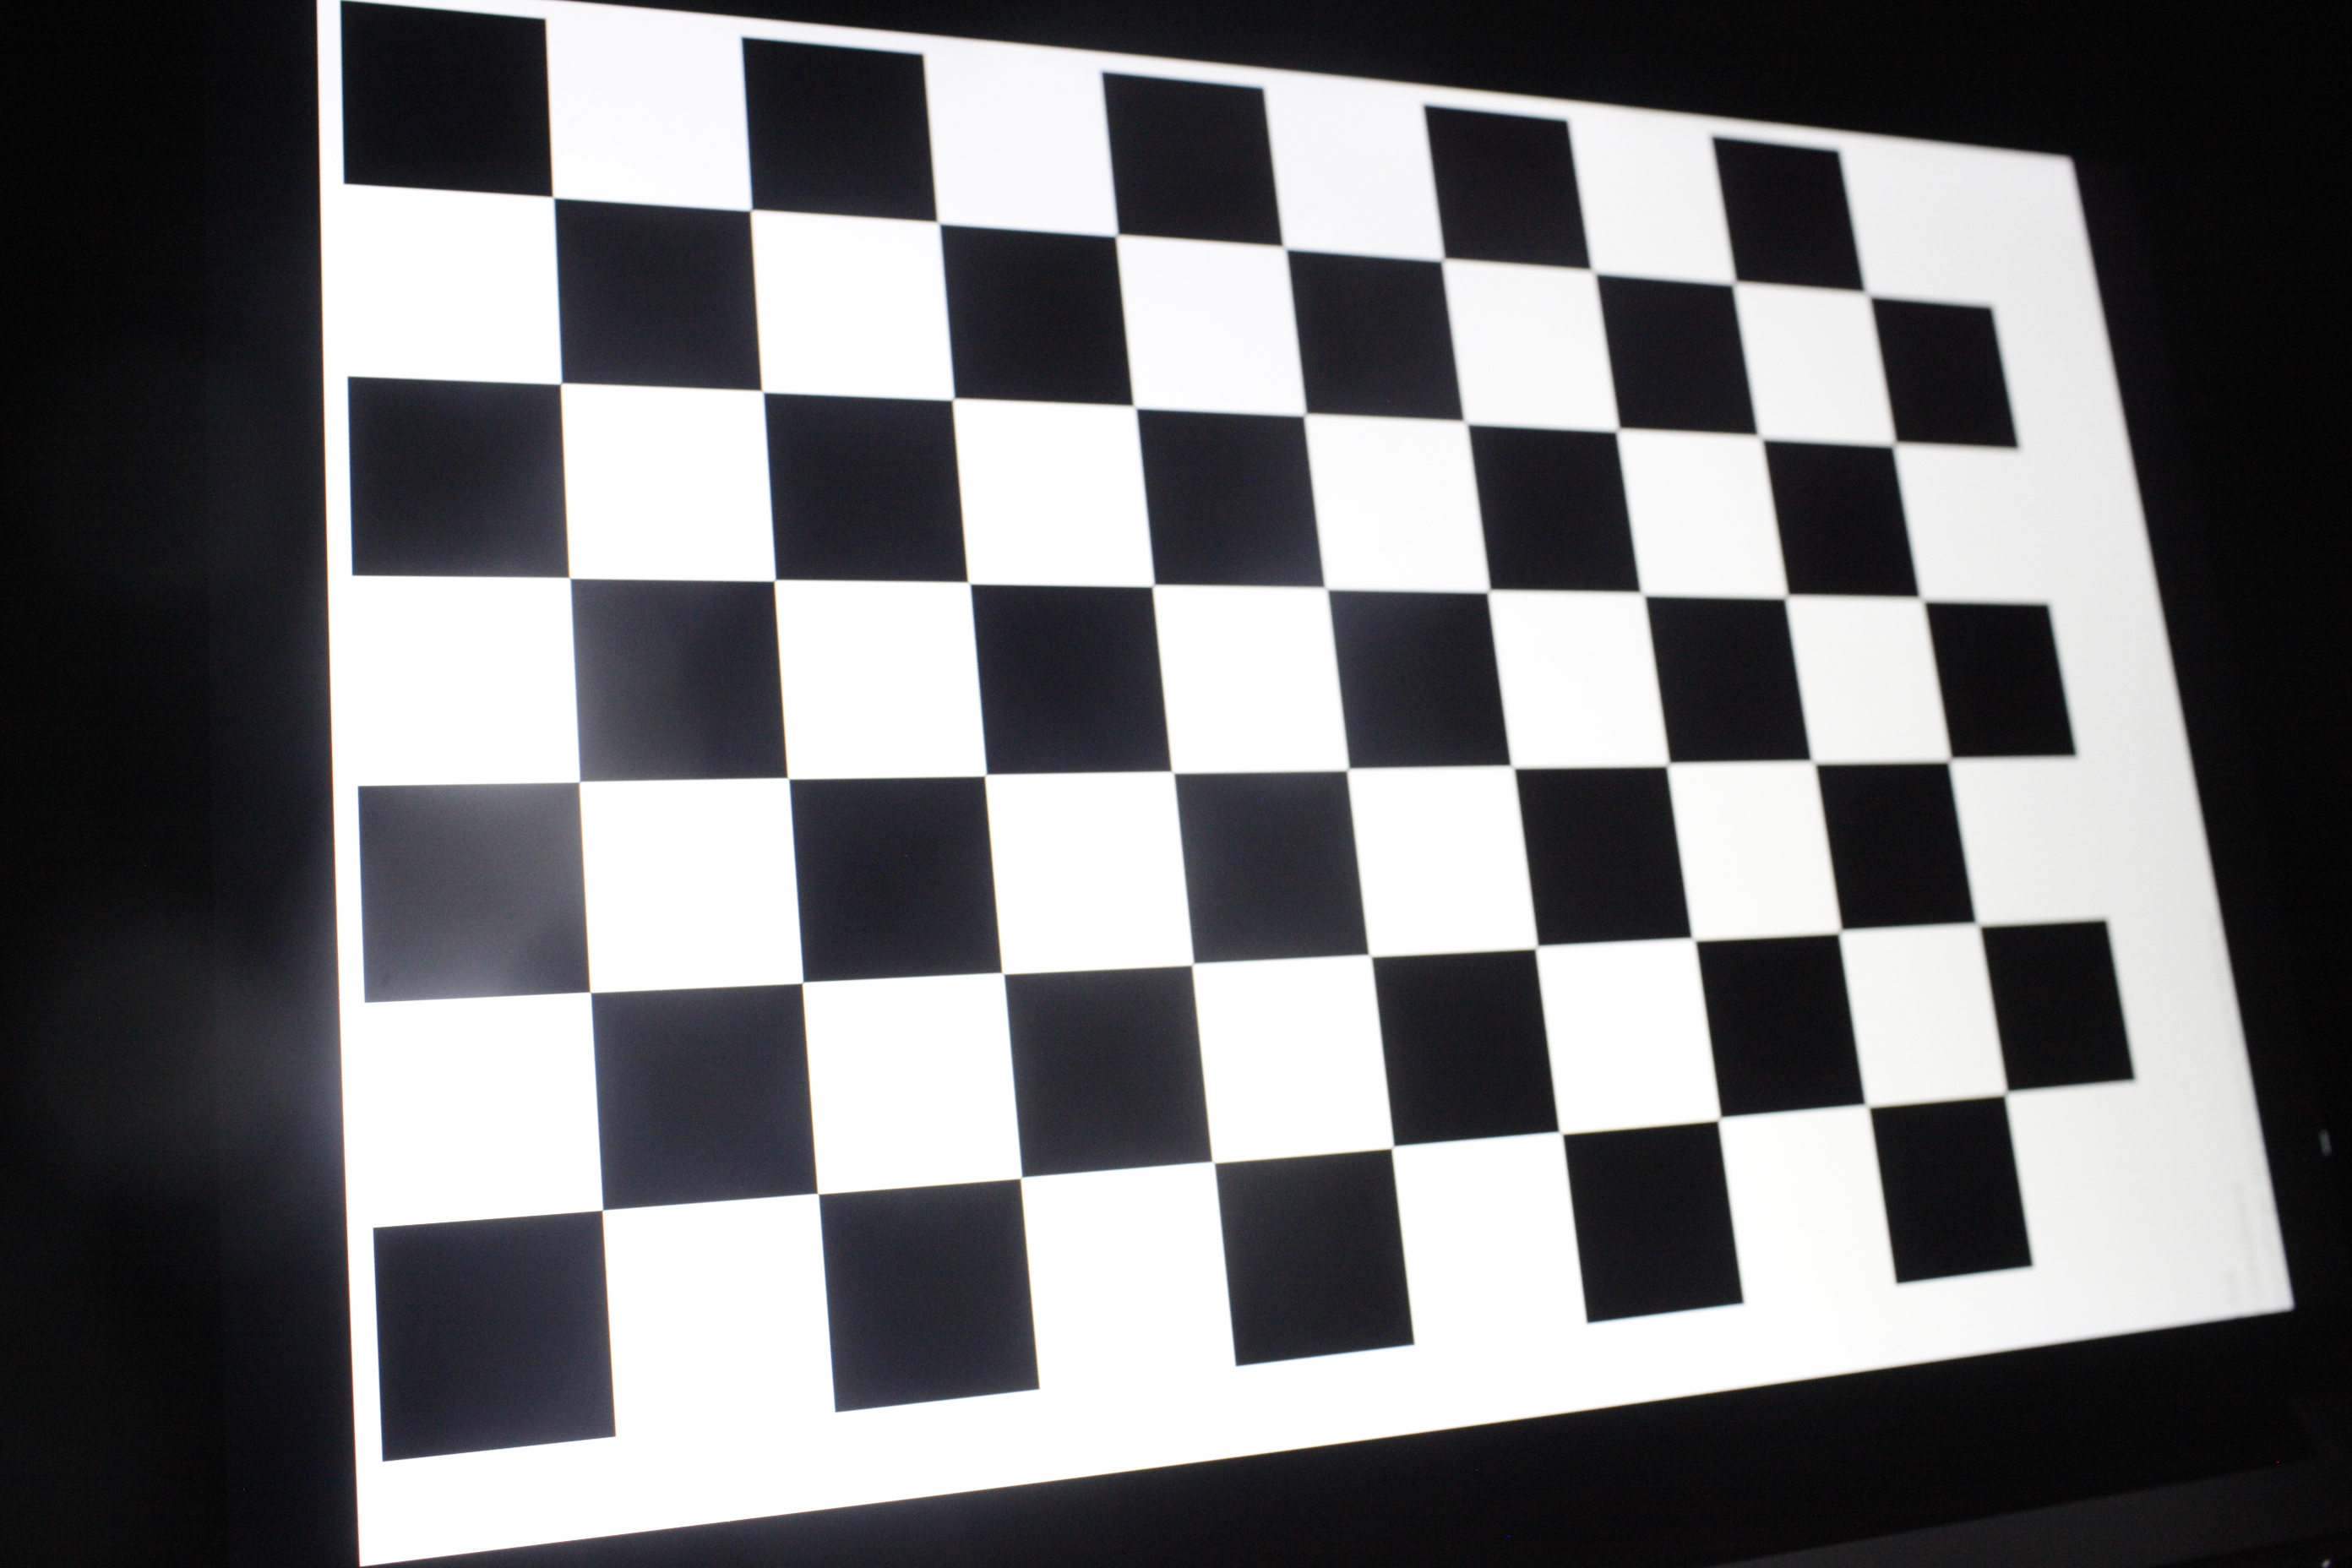
\includegraphics[width=.3\columnwidth]{images/chessboard/p11}
}
\subfigure[Image 12]{
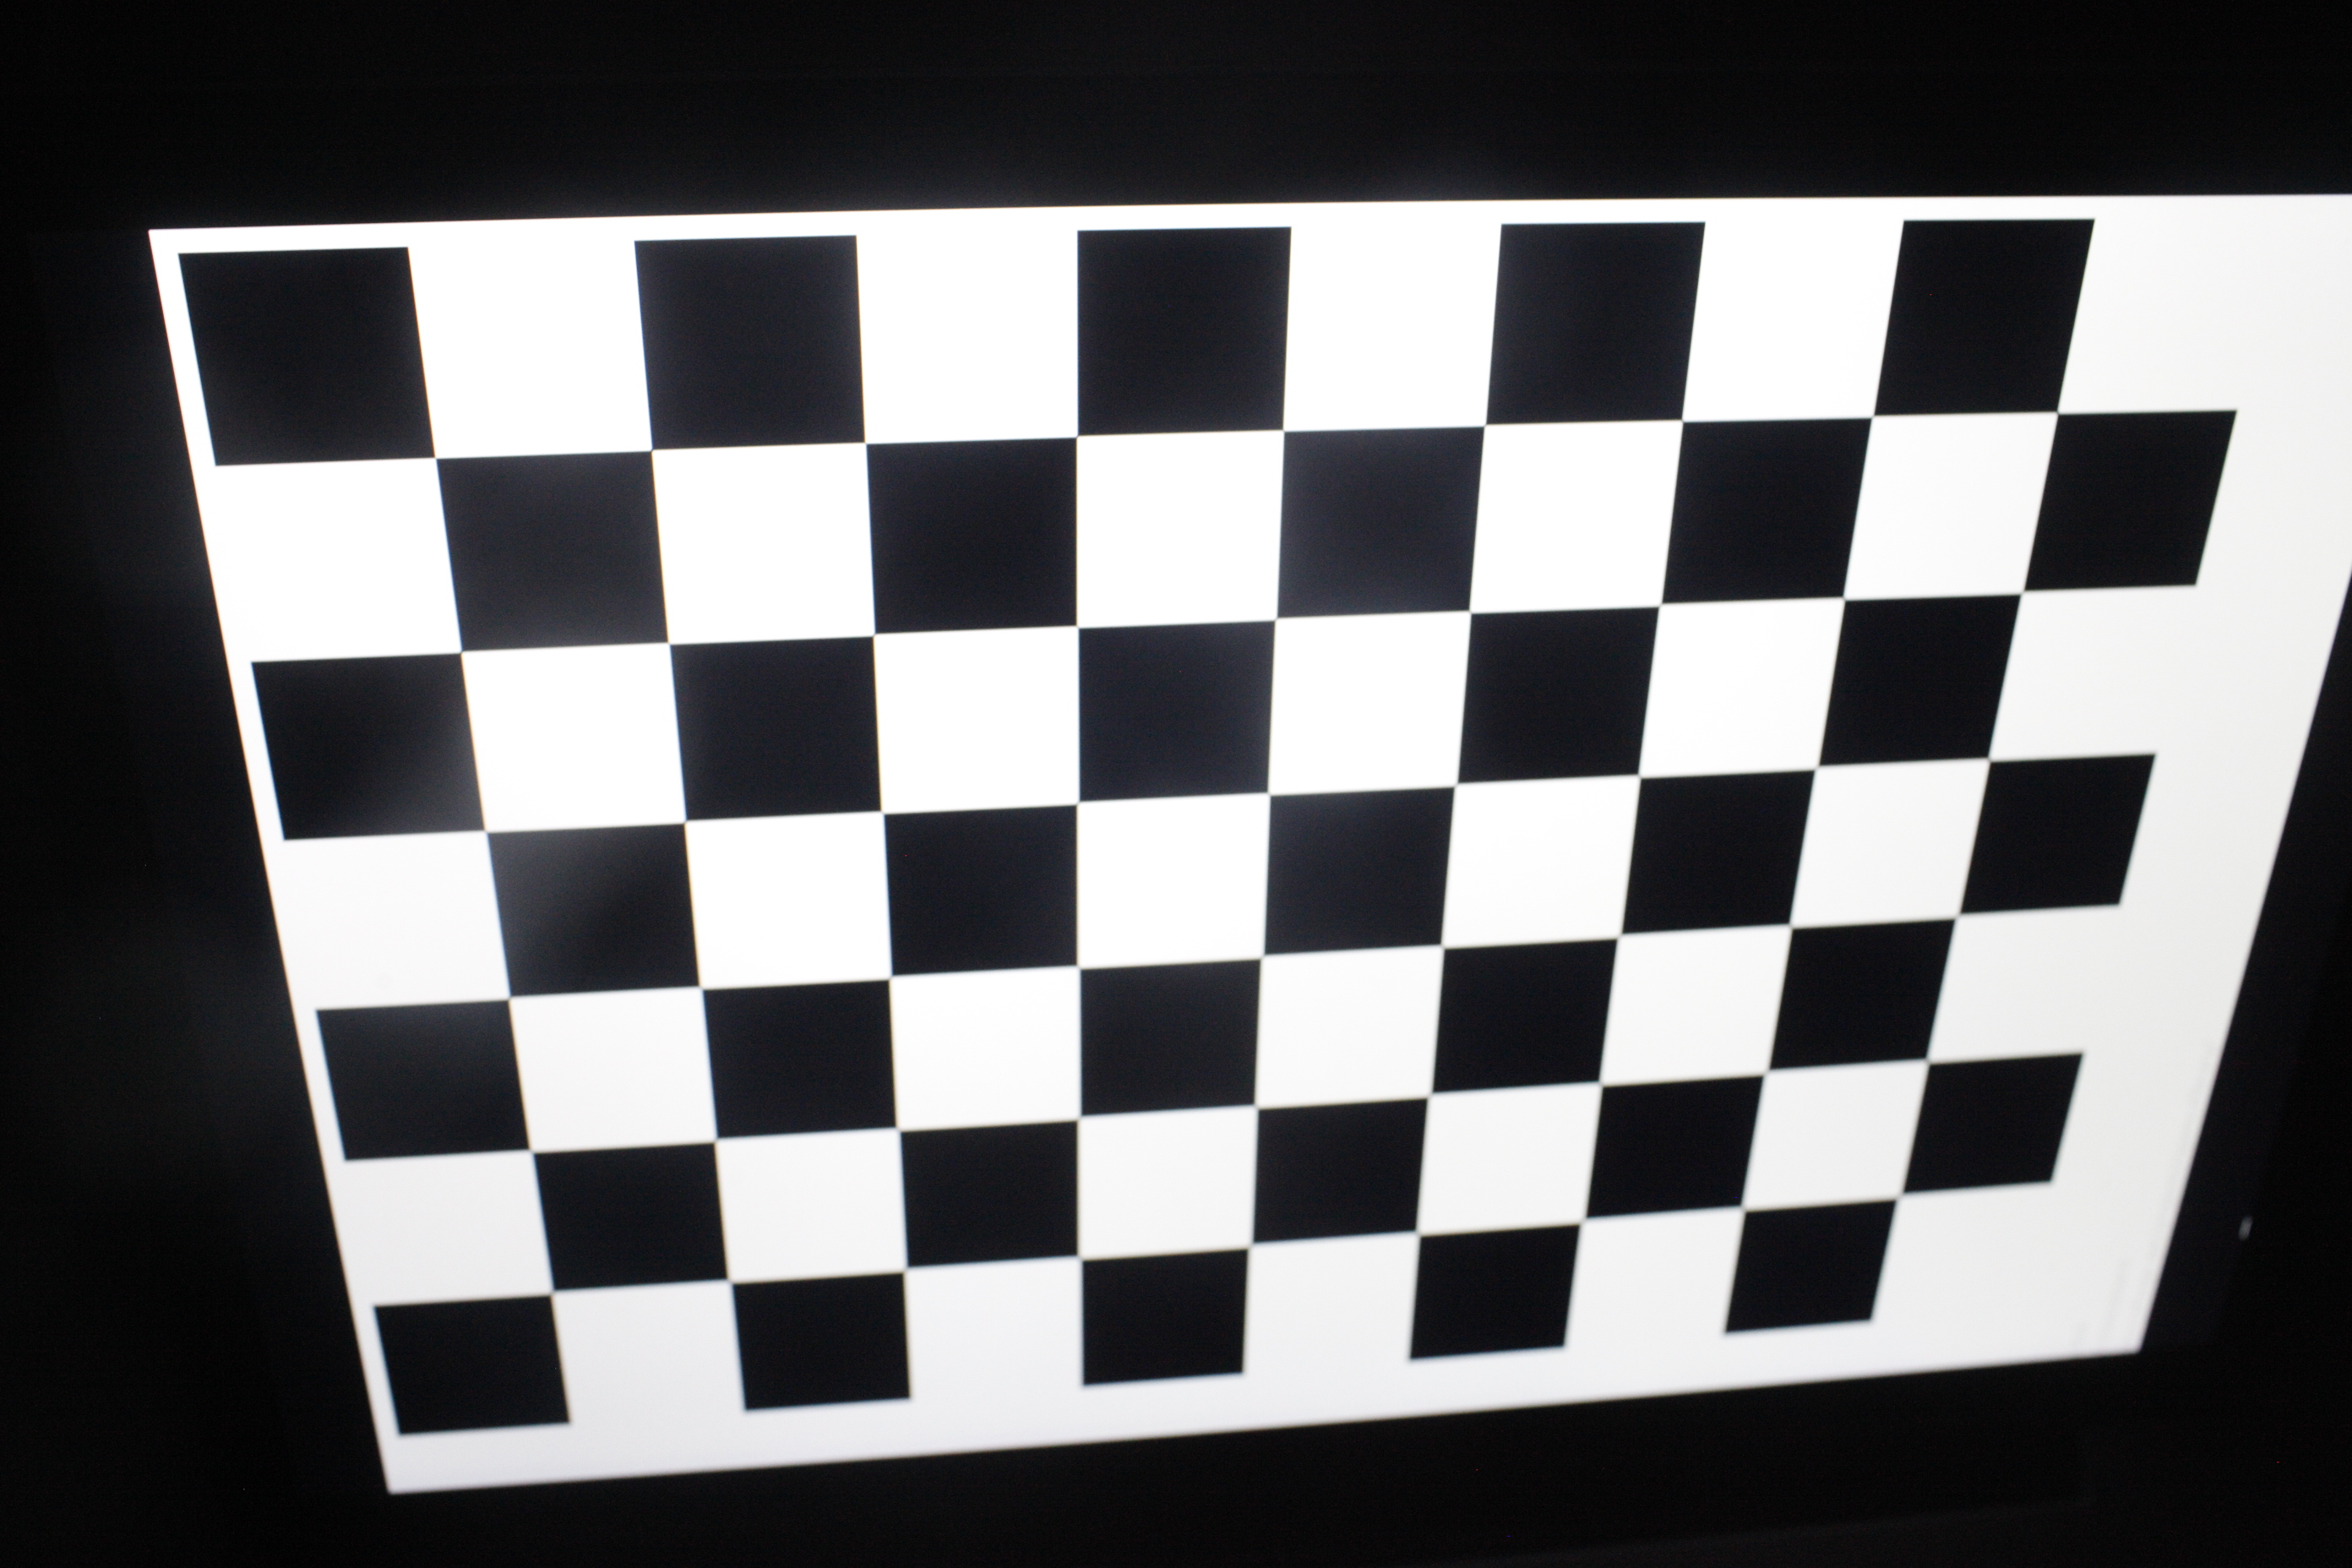
\includegraphics[width=.3\columnwidth]{images/chessboard/p12}
}


\caption{Chessboard Pictures taken from different view points}
\label{fig:chessboard}
\end{figure}


\section{Take the pictures}

We use the same camera and lens take 3 pictures as shown in Figure \ref{fig:pictures}. We placed some objects in the front and also left enough distant background.
\begin{figure}[t]
\centering
\subfigure[Image 1]{
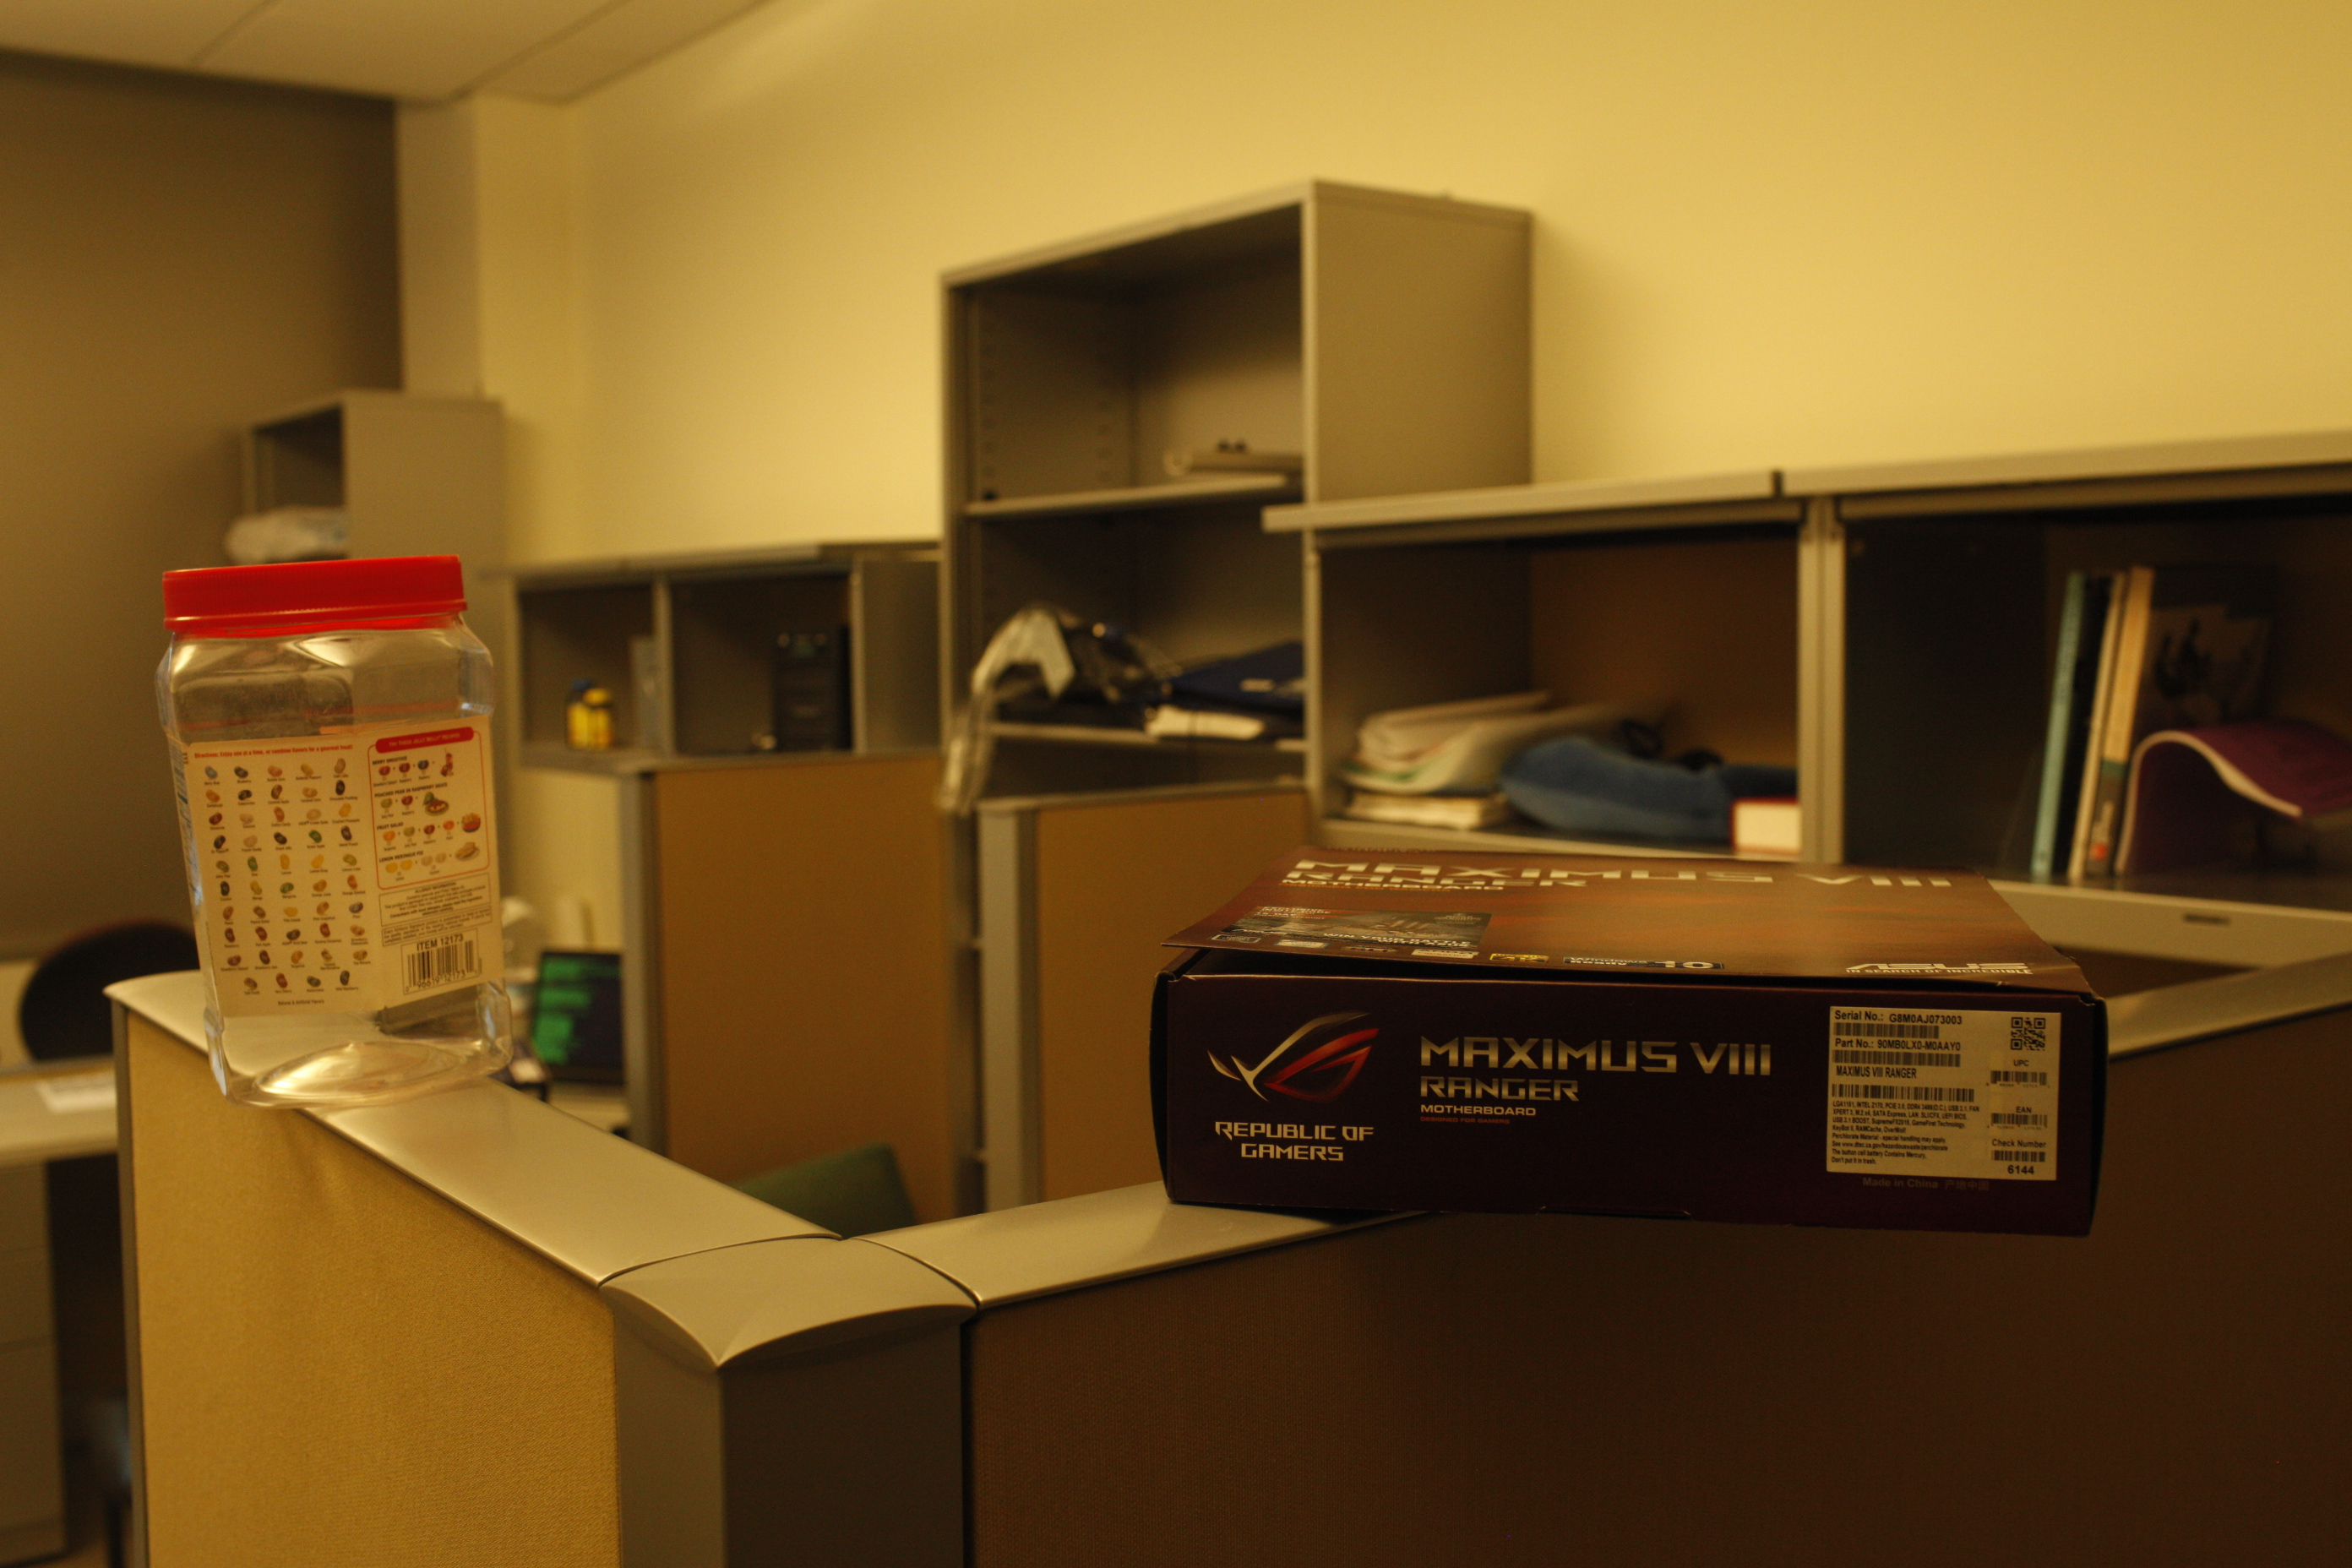
\includegraphics[width=.3\columnwidth]{images/multiview/p1}
}
\subfigure[Image 2]{
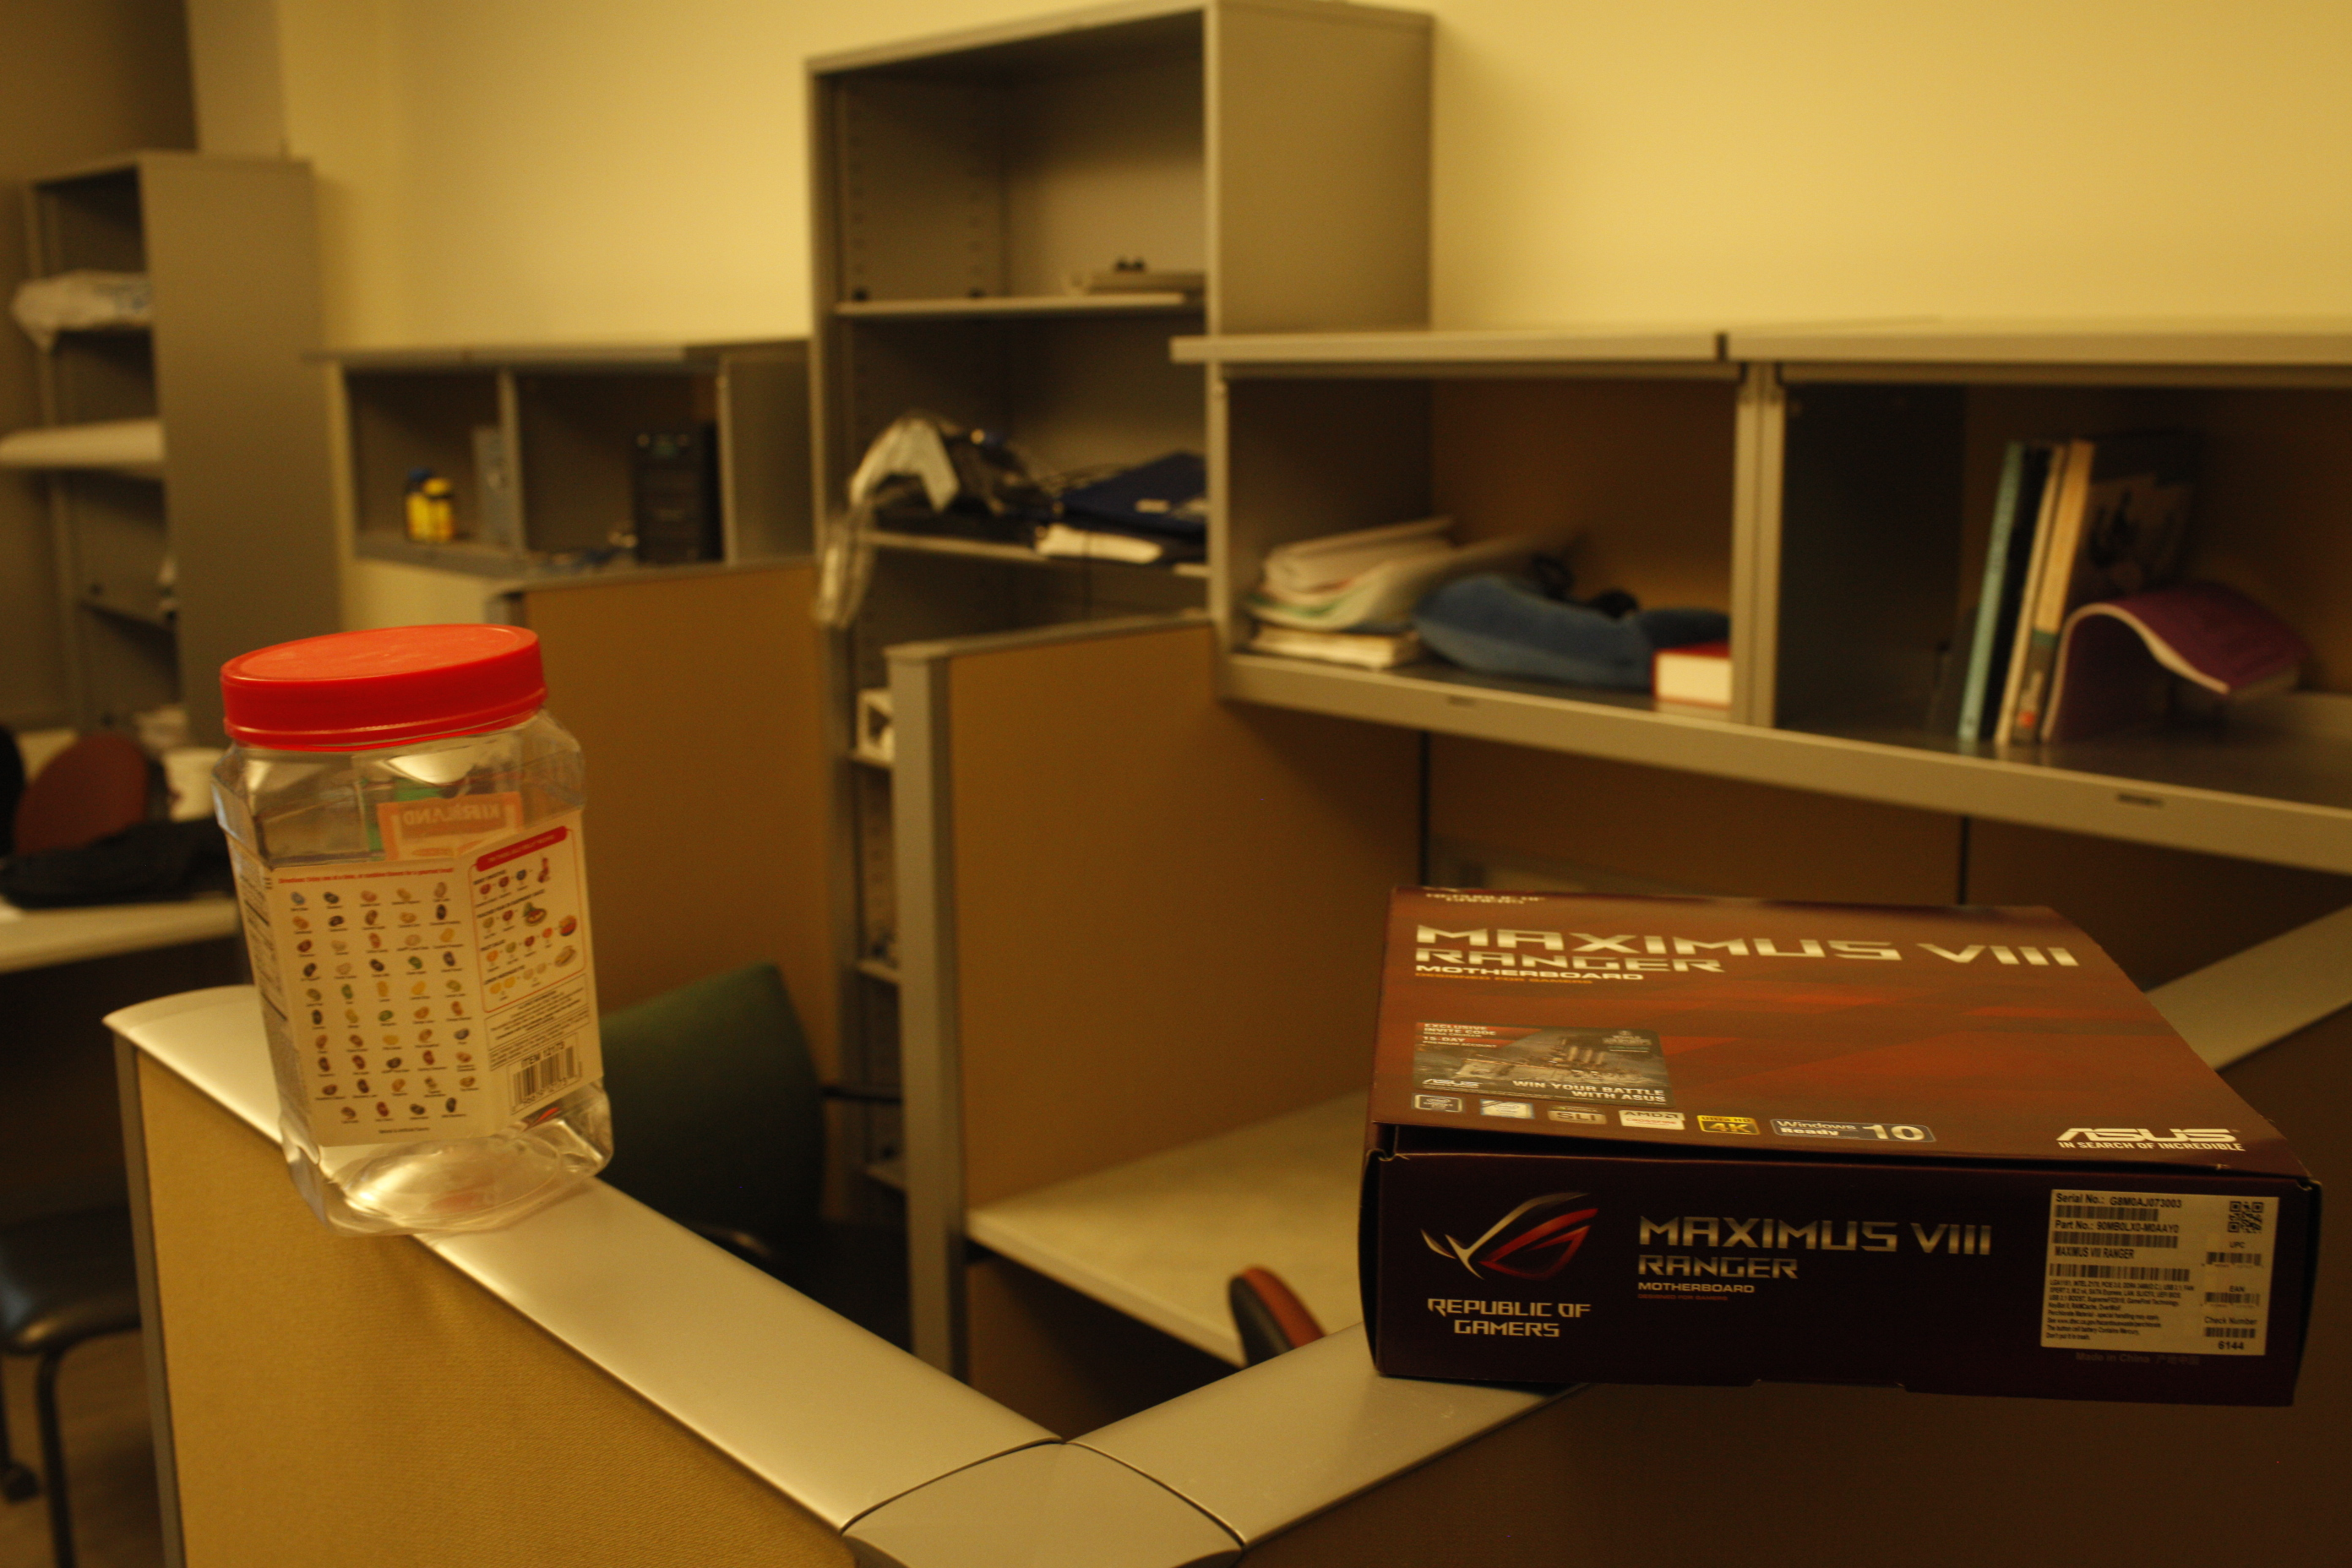
\includegraphics[width=.3\columnwidth]{images/multiview/p2}
}
\subfigure[Image 3]{
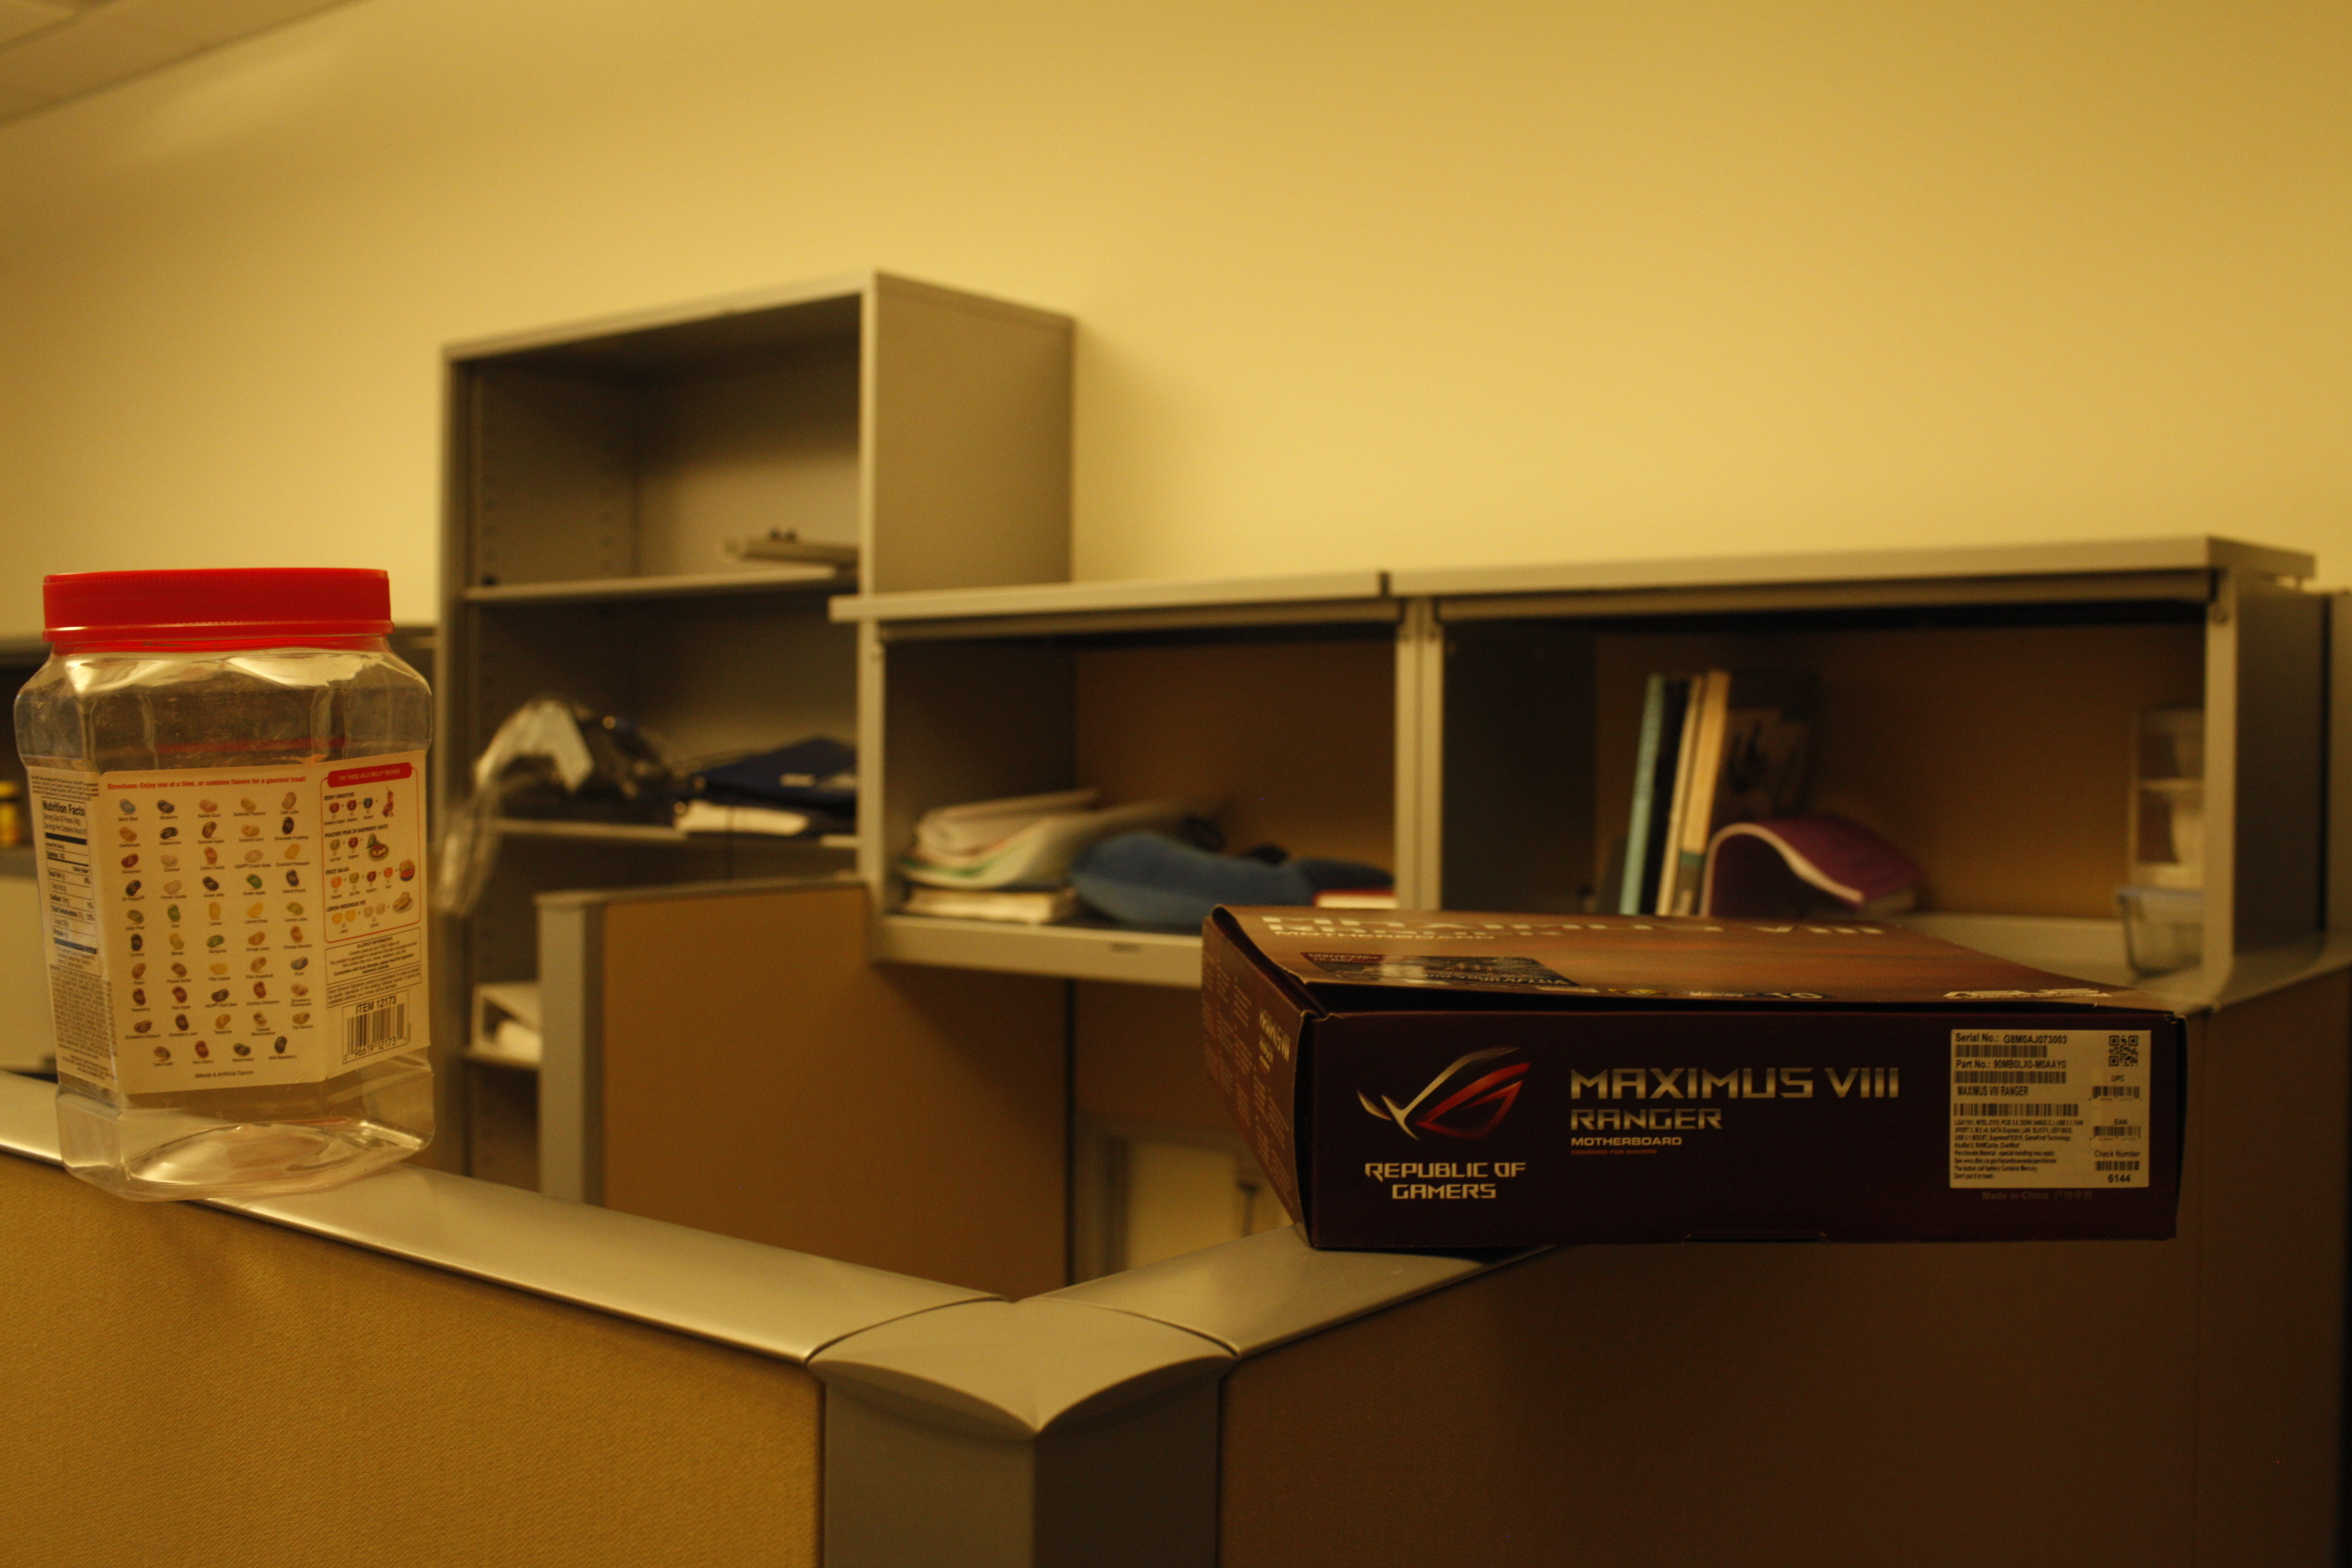
\includegraphics[width=.3\columnwidth]{images/multiview/p3}
}

\caption{Pictures taken from different distances and directions}
\label{fig:pictures}
\end{figure}

\section{Compute the essential matrix of all three camera pairs}

We first undistort pictures with calibration parameters as shown in Figure. There were 25 pixels loss in height and 12 pixels loss in width. Straight lines in those images confirms the calibration was done correctly.\\

In order to get pixel pairs over 3 camera pairs, we built a tool to allow us to pick those pixel pairs by hand. Figure \ref{fig:undistorted} shows the interface of our tool.\\

For each camera pair, we picked 17 to 18 pixel pairs to provide enough data calculating essential matrices and fundamental matrices. Figure \ref{fig:epipolar} shows the pixel pairs we picked over 3 camera pairs.\\

The essential matrices we calculated are

$$\textbf{E}_{12} =
\begin{bmatrix}
-2.944{\text e-}07&-1.993{\text e-}06&2.051{\text e-}02\\
3.242{\text e-}06&-9.280{\text e-}07&-2.045{\text e-}02\\
-2.030{\text e-}02&1.995{\text e-}02&1.000{\text e+}00 
\end{bmatrix}
$$

$$\textbf{E}_{13} =
\begin{bmatrix}
4.323{\text e-}08&1.144{\text e-}06&-1.610{\text e-}03\\
-2.850{\text e-}07&2.763{\text e-}07&-7.243{\text e-}03\\
5.939{\text e-}04&5.592{\text e-}03&1.000{\text e+}00
\end{bmatrix}
$$

$$\textbf{E}_{23} =
\begin{bmatrix}
1.608{\text e-}07&2.496{\text e-}07&-2.468{\text e-}03\\
-1.274{\text e-}07&1.268{\text e-}08&-1.230{\text e-}03\\
1.877{\text e-}03&9.439{\text e-}04&1.000{\text e+}00
\end{bmatrix}
$$


\begin{figure}[t]
\centering
\subfigure[Image 1]{
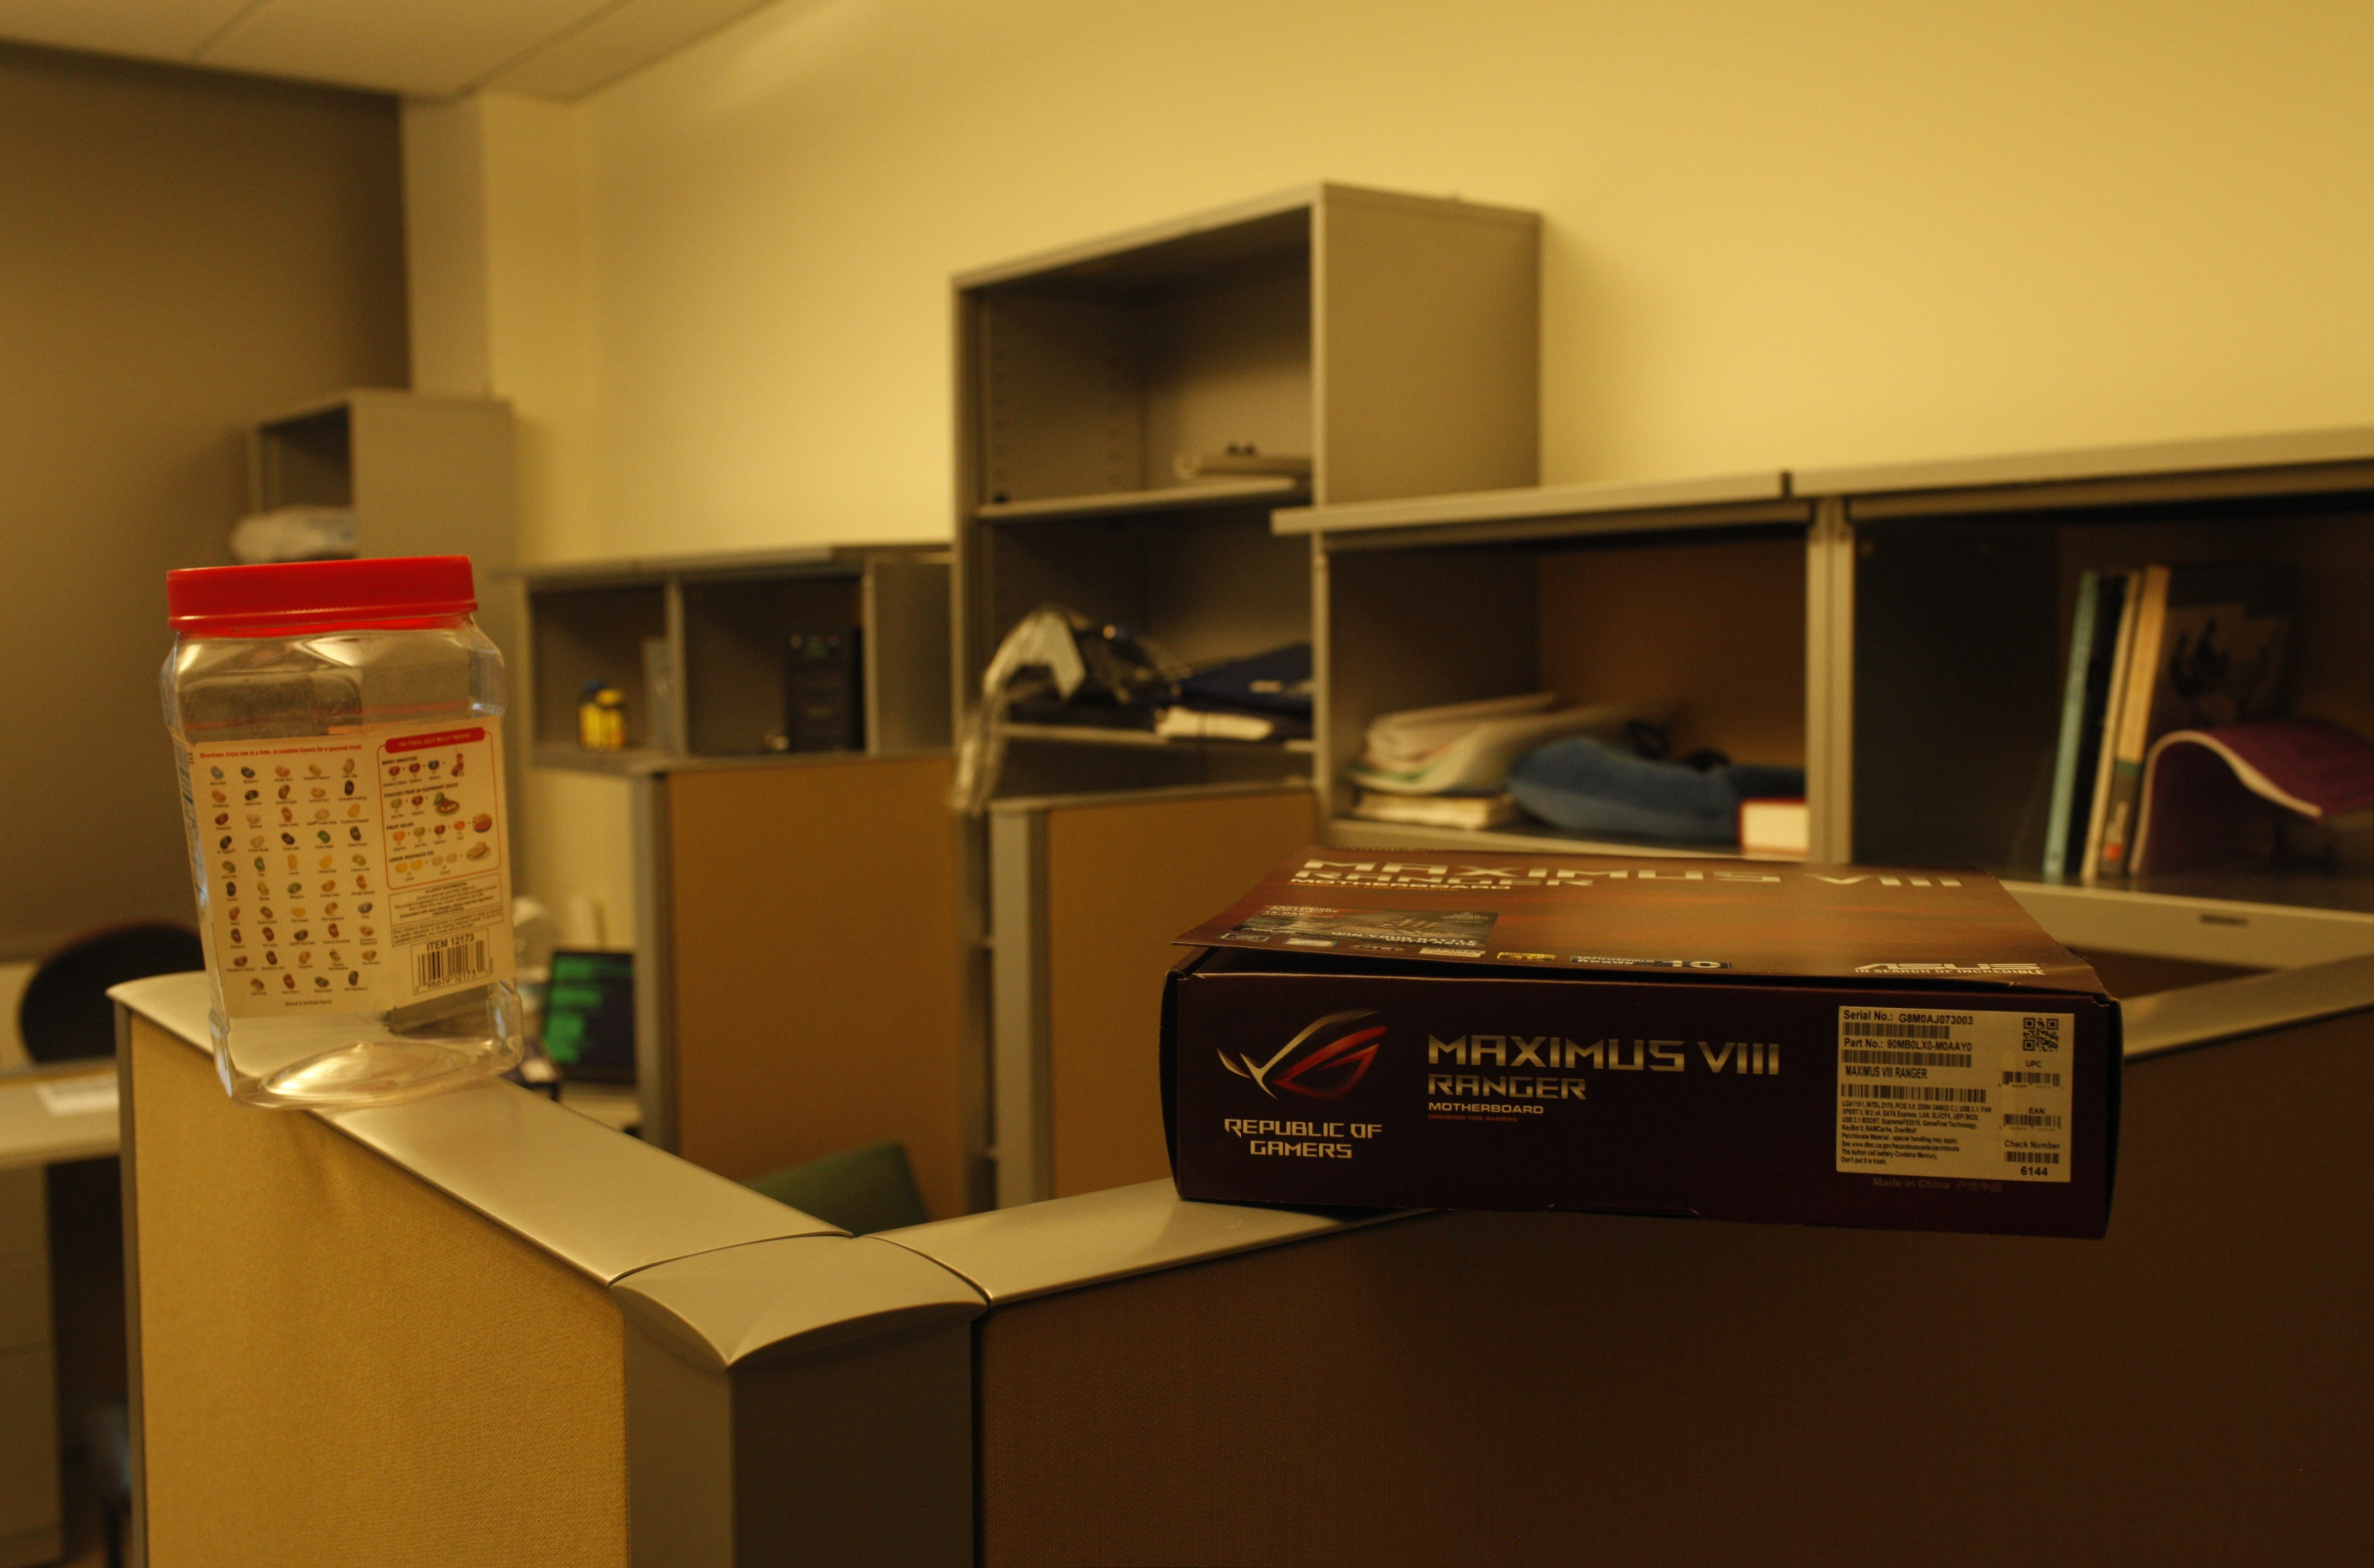
\includegraphics[width=.3\columnwidth]{images/undistorted/p1}
}
\subfigure[Image 2]{
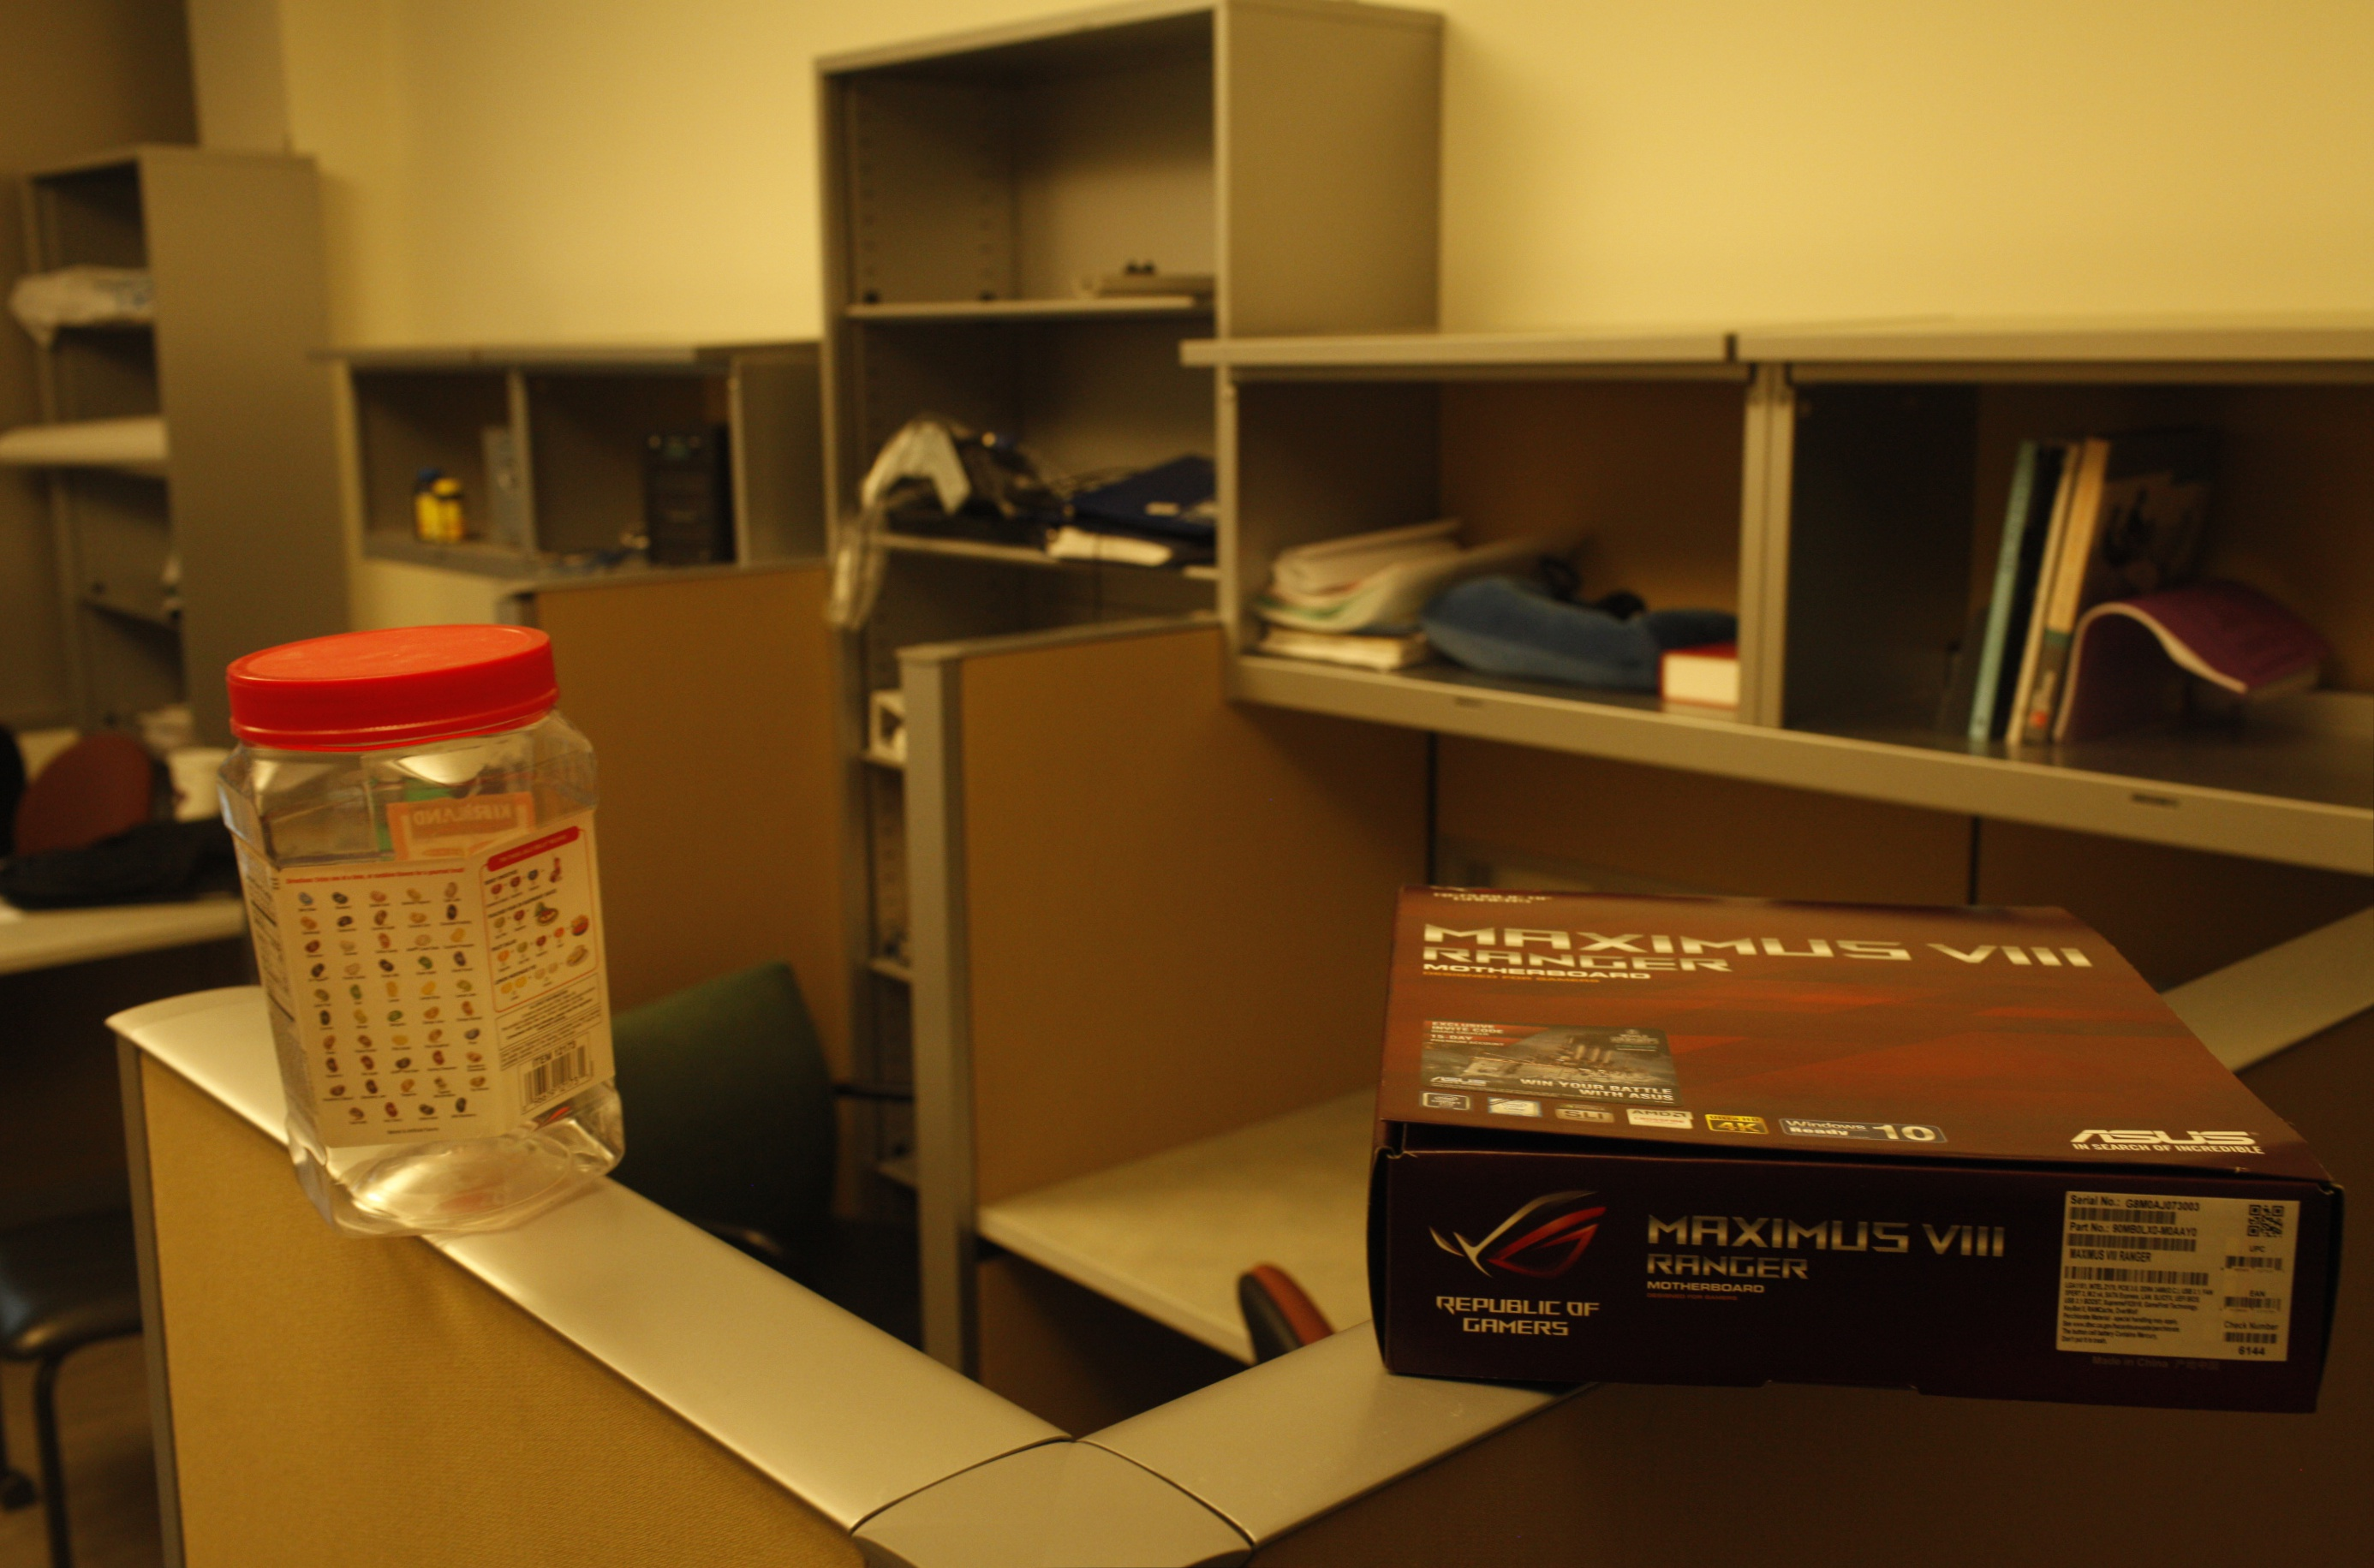
\includegraphics[width=.3\columnwidth]{images/undistorted/p2}
}
\subfigure[Image 3]{
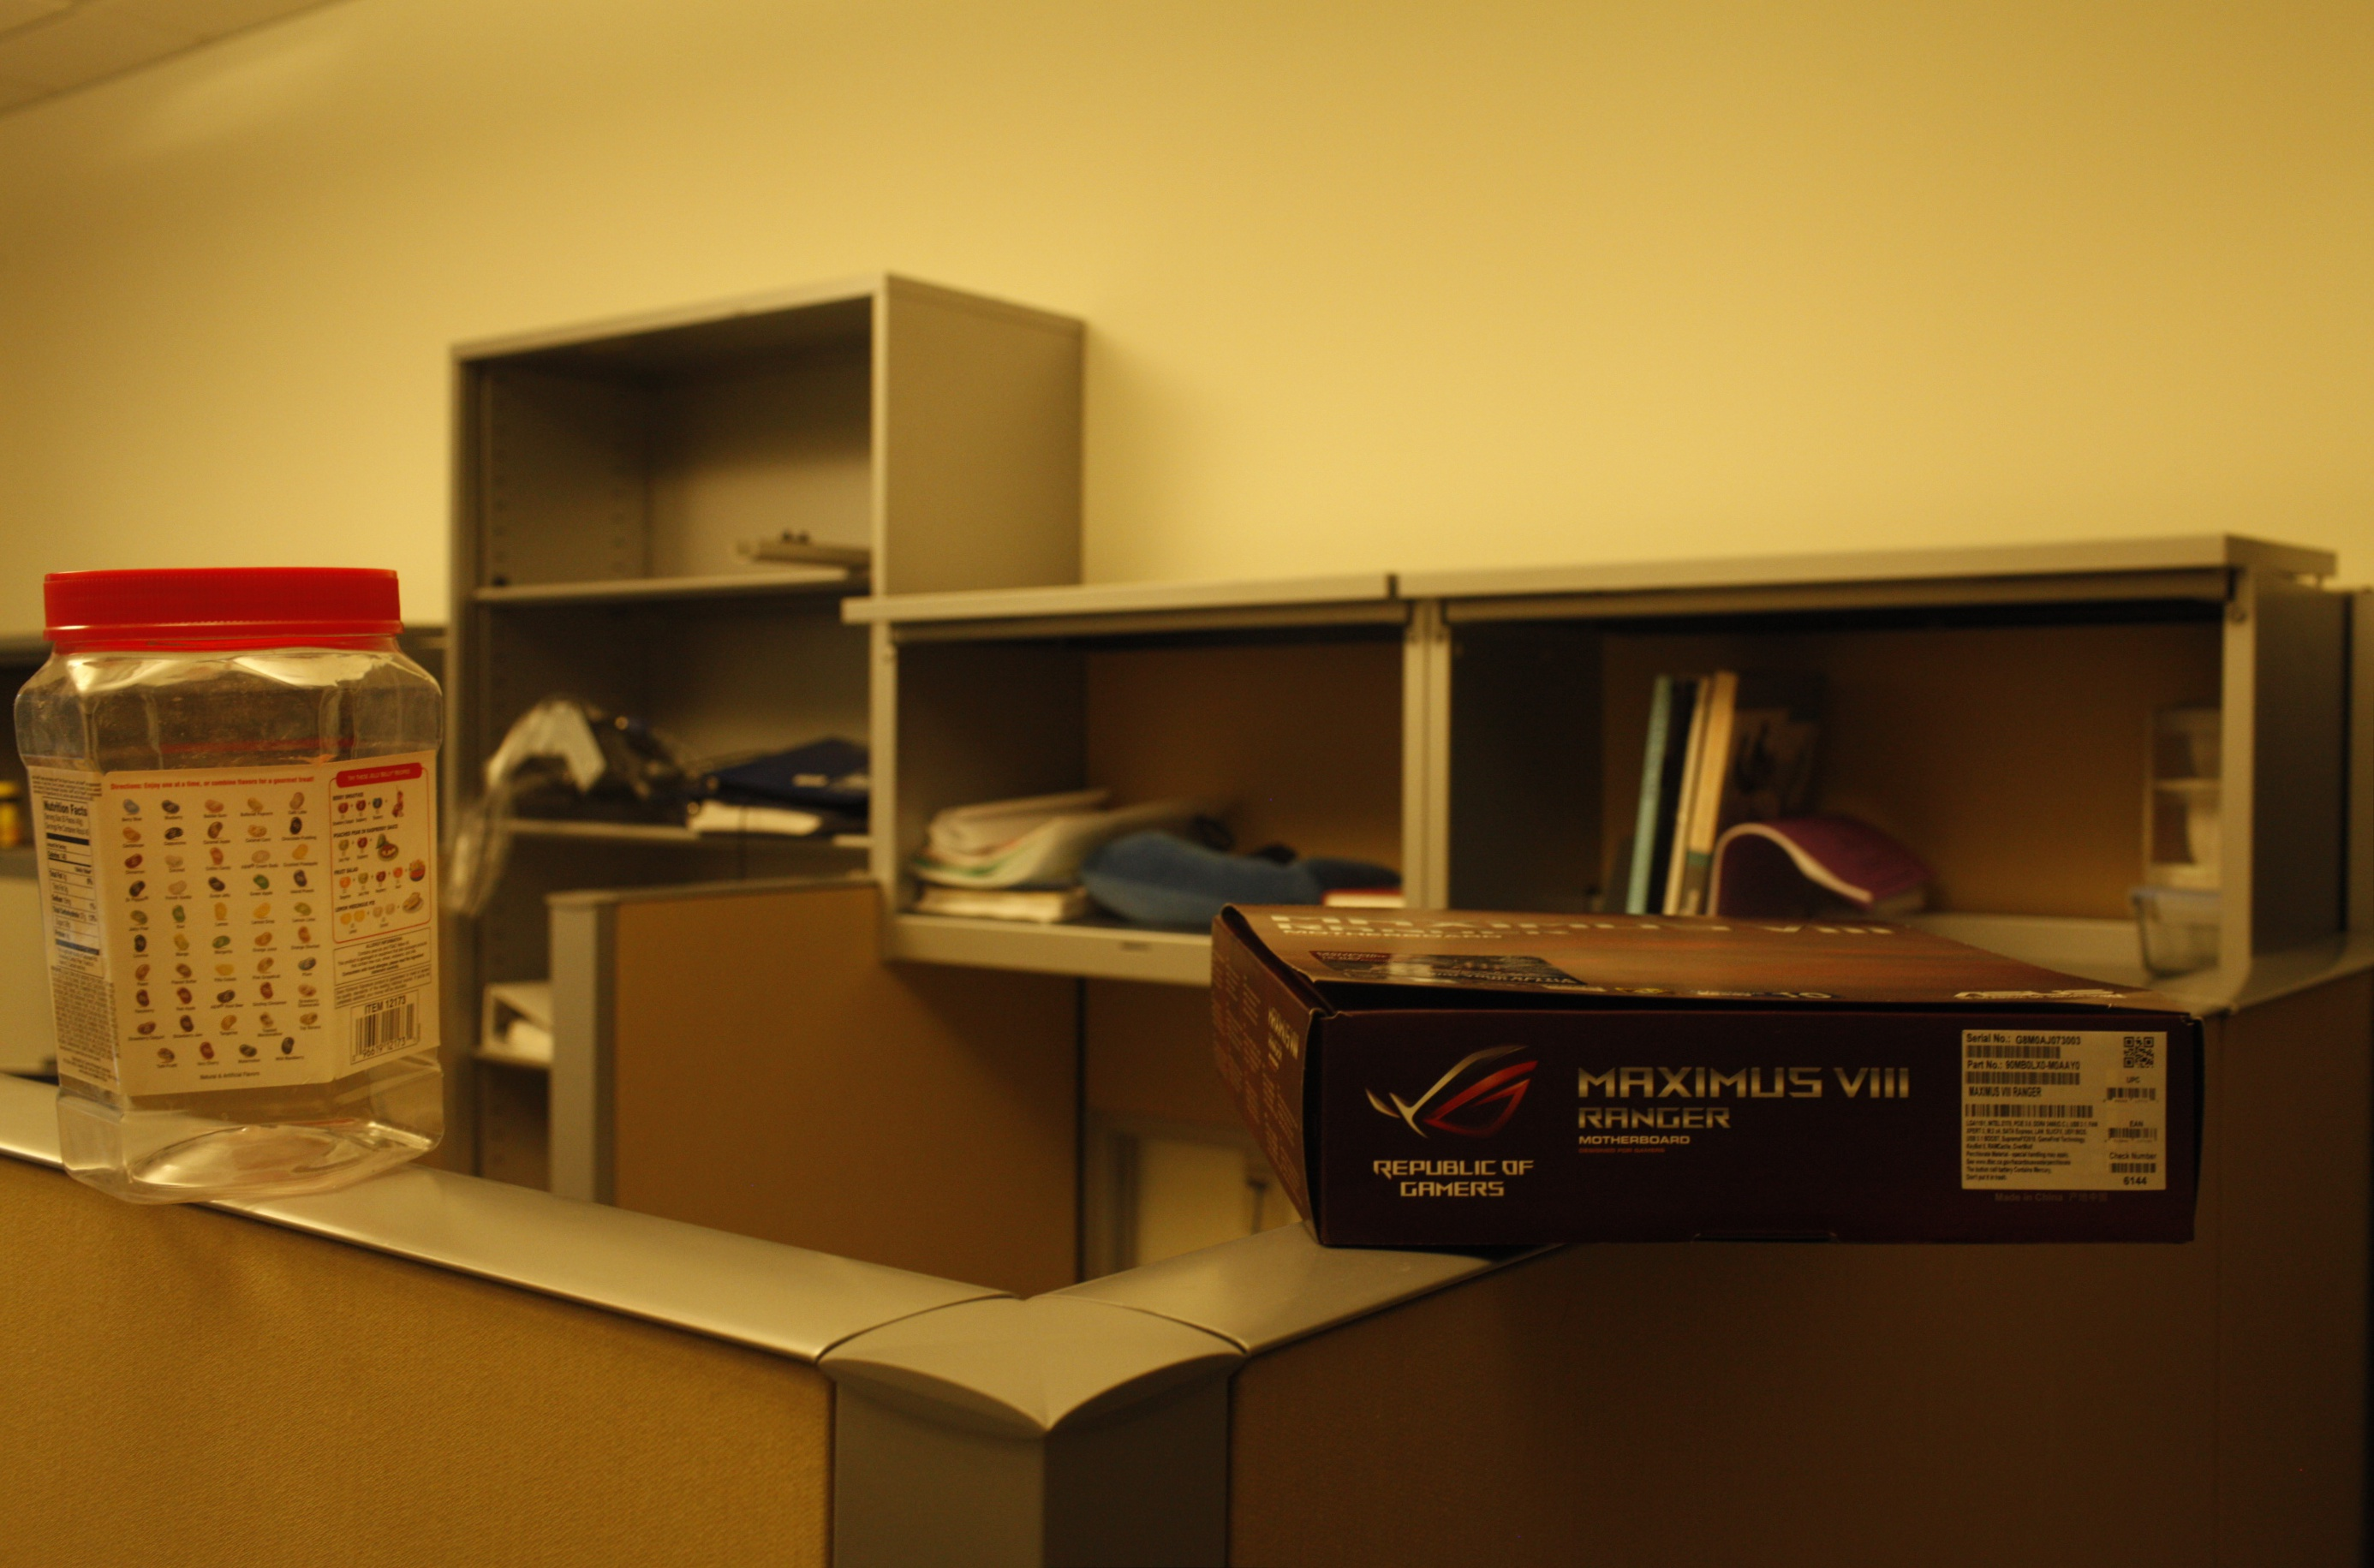
\includegraphics[width=.3\columnwidth]{images/undistorted/p3}
}

\caption{Undistorted pictures.}
\label{fig:undistorted}
\end{figure}


\begin{figure}[t]
\centering
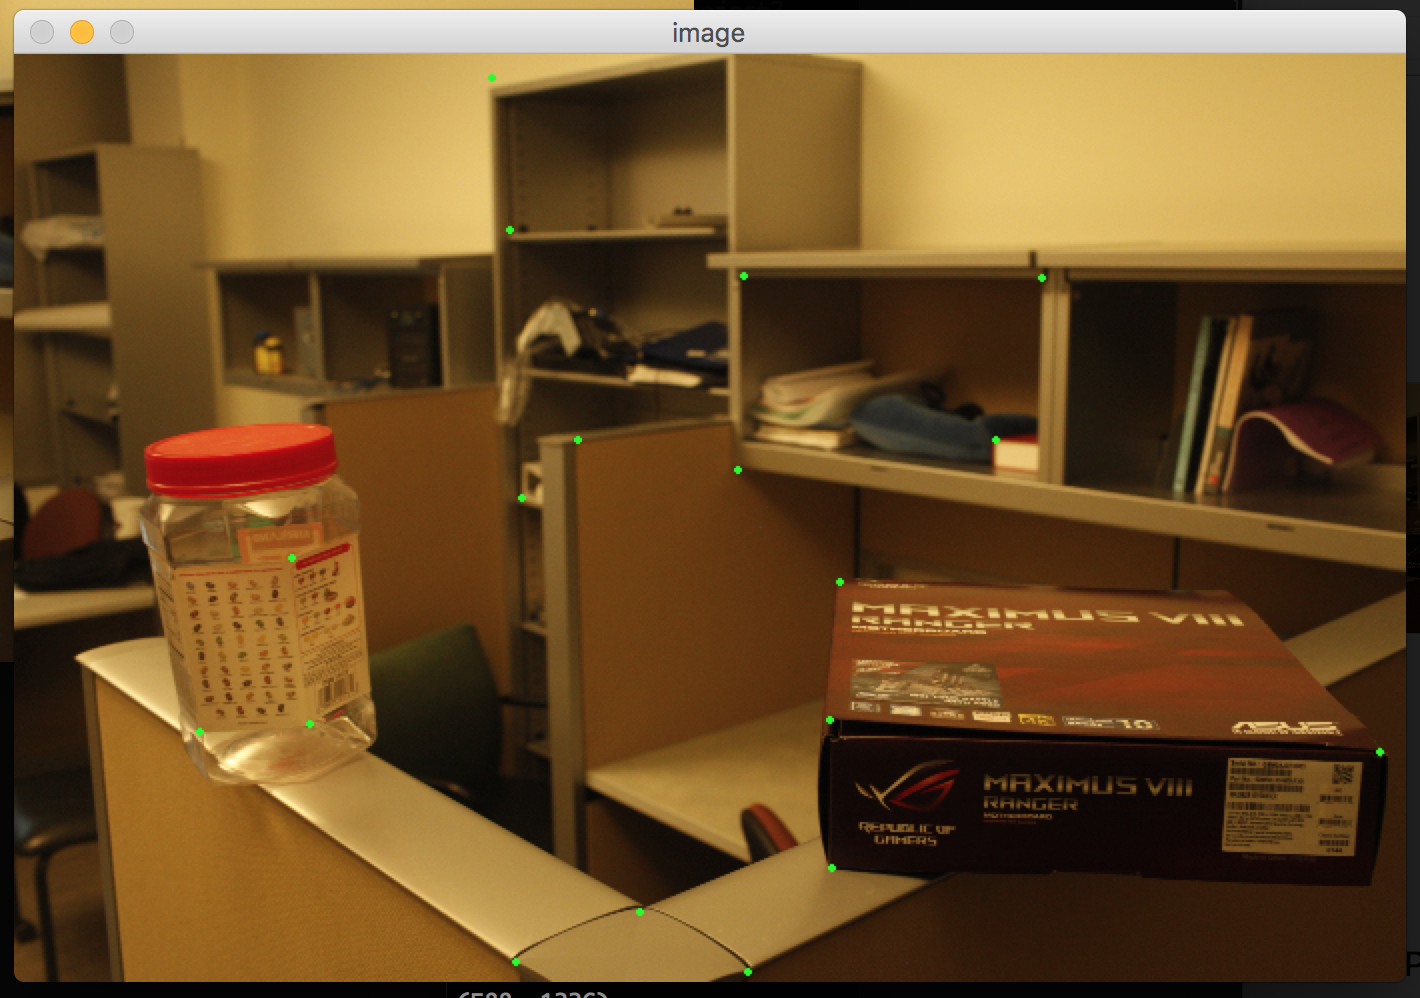
\includegraphics[width=\columnwidth]{images/pick}

\caption{Pictures taken from different distances and directions}
\label{fig:pick}
\end{figure}

\begin{figure}[t]
\centering
\subfigure[Image 1 - Image 2]{
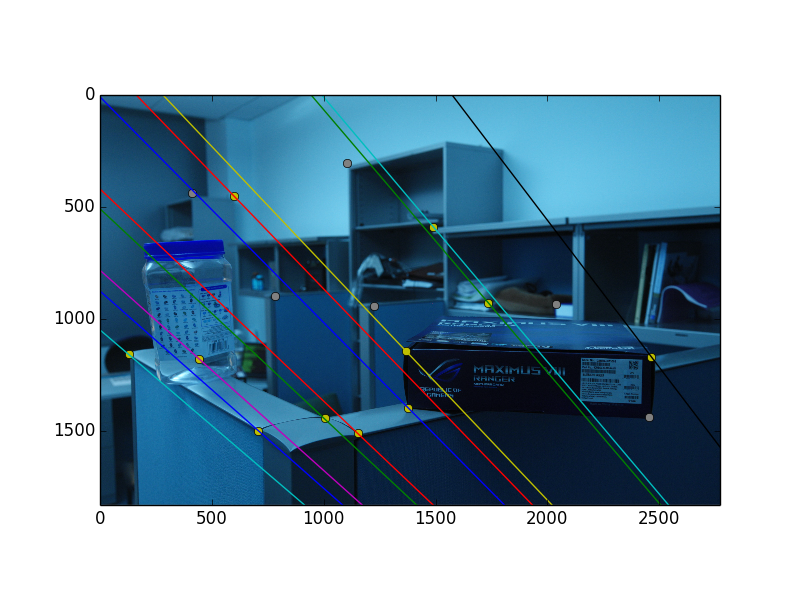
\includegraphics[width=.45\columnwidth]{images/epipolar/1-2-1}
}
\subfigure[Image 2 - Image 1]{
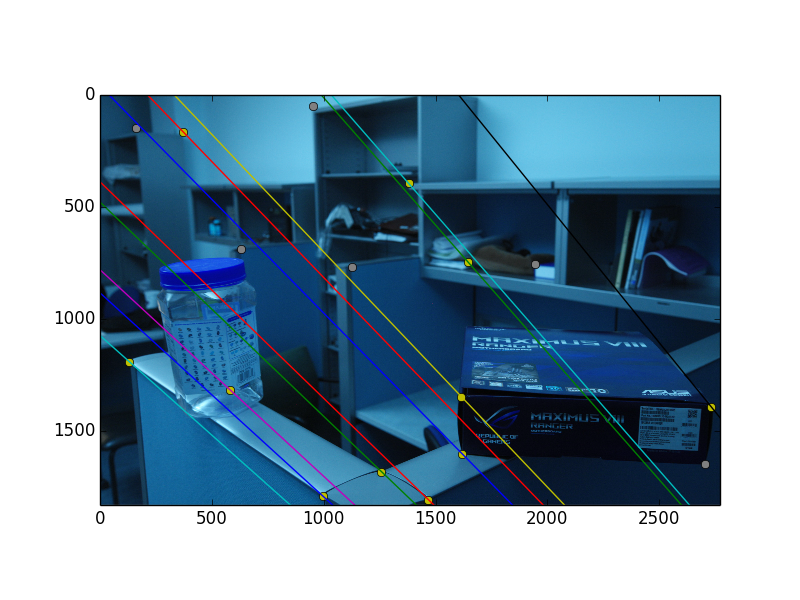
\includegraphics[width=.45\columnwidth]{images/epipolar/1-2-2}
}
\subfigure[Image 1 - Image 3]{
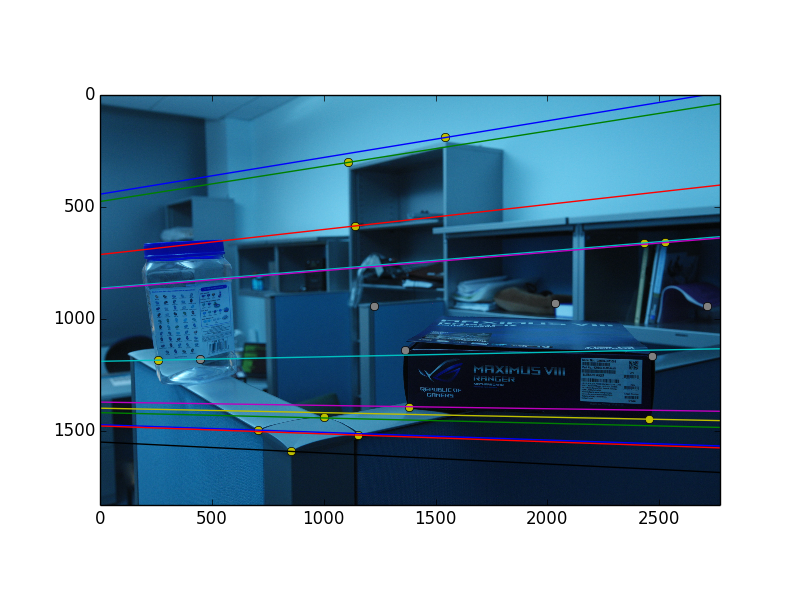
\includegraphics[width=.45\columnwidth]{images/epipolar/1-3-1}
}
\subfigure[Image 3 - Image 1]{
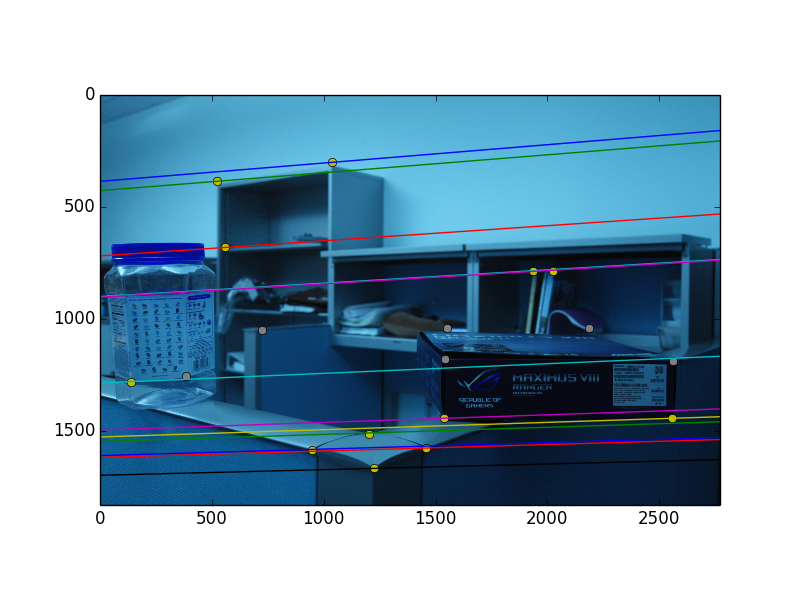
\includegraphics[width=.45\columnwidth]{images/epipolar/1-3-3}
}
\subfigure[Image 2 - Image 3]{
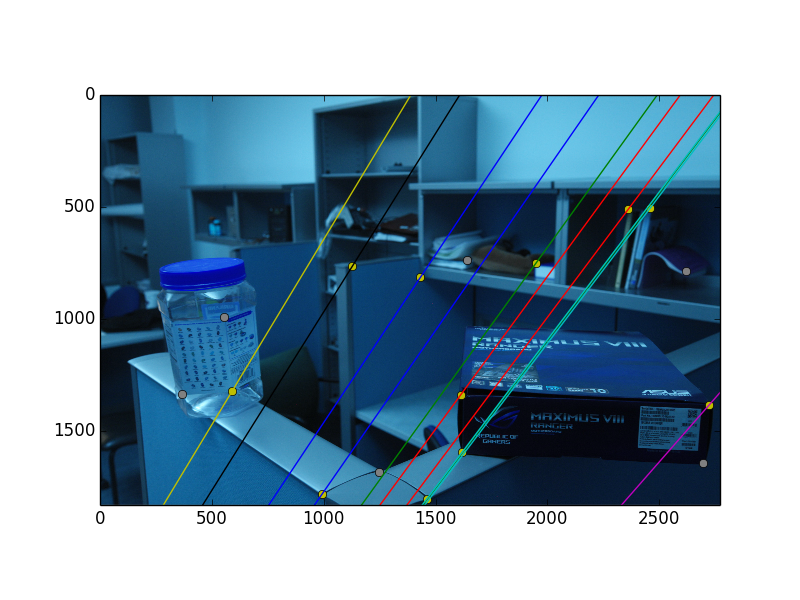
\includegraphics[width=.45\columnwidth]{images/epipolar/2-3-2}
}
\subfigure[Image 3 - Image 2]{
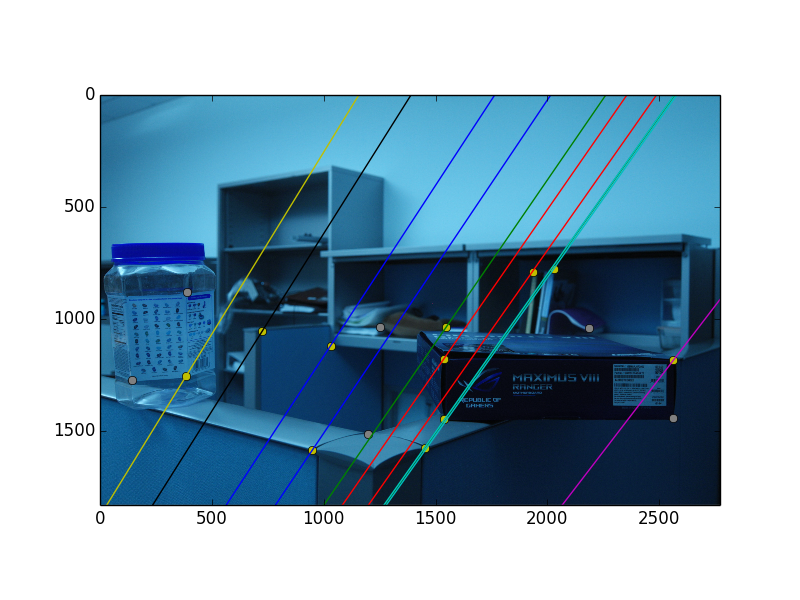
\includegraphics[width=.45\columnwidth]{images/epipolar/2-3-3}
}

\caption{Hand-pick pixel pairs (Inliers are yellow while outliers are gray) and corresponding epipolar lines.}
\label{fig:epipolar}
\end{figure}

\section{Find the extrinsic parameters}


\section{Rescale the translation vector}
After we have found the extrinsic parameters, we obtained the rotation matrices $\textbf{R}_{1}^{2}$, $\textbf{R}_{2}^{3}$, $\textbf{R}_{1}^{3}$, we also obtained the vector $\textbf{r}_{12}^{1}$ representing camera 2 seen by the camera 1, expressed in reference of the camera 1. The same to vector $\textbf{r}_{23}^{2}$ and vector $\textbf{r}_{13}^{1}$ we obtained.

In this part, the first work we did is to express the vectors in terms of a common reference frame. We choose the camera 1 reference system as the common reference system, we obtain $\textbf{r}_{23}^{1}$ by doing matrix multiplication on transpose matrix of $\textbf{R}_{1}^{2}$ and vector $\textbf{r}_{23}^{2}$. We can also have $\textbf{r}_{31}^{1} = - \textbf{r}_{13}^{1}$. Now we have $\textbf{r}_{12}^{1}$, $\textbf{r}_{31}^{1}$ and $\textbf{r}_{31}^{1}$, all the 3 vectors are to the same common reference system.

The next work we do on is to convert all the 3 vectors to unit form. We divided all the 3 vector by their length respectively. Now we have $\textbf{r}_{12unit}^{1}$, $\textbf{r}_{23unit}^{1}$ and $\textbf{r}_{31unit}^{1}$. 

After the mathematics performed by the project guidance, we have the formula $| \textbf{r}_{12unit}^{1} + \beta  \textbf{r}_{23unit}^{1} + \gamma  \textbf{r}_{31unit}^{1} |$. In an ideal world, the $| \textbf{r}_{12unit}^{1} + \beta  \textbf{r}_{23unit}^{1} + \gamma  \textbf{r}_{31unit}^{1} |$ should equal to $0$, however in practice due to the error and noise, we just can minimize the value as small as possible. We use the $minimize()$ function imported from $scipy.optimize$ to do the minimization and find the $\beta$ and $\gamma$ value such that the $| \textbf{r}_{12unit}^{1} + \beta  \textbf{r}_{23unit}^{1} + \gamma  \textbf{r}_{31unit}^{1} |$ value is minimized.

The outcome of the optimization gave us the value  $\beta = $ and $\gamma = $, we can also see that by this time $| \textbf{r}_{12unit}^{1} +  \textbf{r}_{23unit}^{1} +  \textbf{r}_{31unit}^{1} | = $ and $| \textbf{r}_{12unit}^{1} + \beta  \textbf{r}_{23unit}^{1} + \gamma  \textbf{r}_{31unit}^{1} | = $, the second is smaller as shown.


\section{Acknowledgment}
We did all the project together. However, Ziqiang Wang is mainly responsible for
Section \ref{sec:create} and Section \ref{sec:reproduce} while Yanan Xie is responsible for the rest parts of this project including providing his professional photography devices.\\

Thanks to \LaTeX\ for providing such a great document preparation system. And many appreciates to the authors of Python, numpy, sklearn, OpenCV and matplotlib.\\



\end{document}
